\section{Identification and Estimation of Life-Cycle Treatment Effects} \label{appendix:methodology}

This appendix presents our approach to identifying and estimating life-cycle treatment effects. Differences in the approach for each outcome are based on different scenarios of data availability. We proceed as follows. Appendix~\ref{app:method_fullobs} focuses on outcomes that are fully observed over the course of the experiment with little attrition. Appendix~\ref{app:method_partialobs} focuses on outcomes that are partially observed over the course of the experiment with a substantial rate of attrition. Appendix~\ref{app:method_noobs}  focuses on outcomes that we do not observe, and thus we need to predict out of sample. Appendices~\ref{app:method_irr} and ~\ref{app:method_cbratio} provide some technical details on the computations of the internal rate of return and the cost-benefit ratios, respectively. Appendix~\ref{appendix:gmm} frames our data combination problem in the Generalized Method of Moments framework. Finally, Appendix~\ref{appendix:bootstrap} provides the precise steps for constructing our statistical inferences.

\subsection{Complete Data}\label{app:method_fullobs}

We classify a variable as complete data when we observe the data for at least 90\% of the individuals in the sample. Table~\ref{table:nonipw} lists the variables that are completely observed. For these outcomes, we estimate the standard errors of our estimates by resampling the ABC/CARE data. We estimate non-parametric $p$-values based on the bootstrap distribution. We perform inference in this same way throughout the paper.

\begin{table}[H]
\begin{threeparttable}
\caption{Variables Estimated without IPW Adjustment}
\label{table:nonipw}
\centering
% CONTENT CREATED ON SPREADSHEET, TREAT AS A .CSV (TAB DELIMITED)
% CAN BE COPIED INTO A SPREADSHEET PROGRAM (EXCEL, LIBRECALC) FOR EDITING
\begin{tabular}{l l}
\toprule
Variable	&	Age	\\
\midrule			
IQ Standard Score	&	2, 3, 4, 5, 6, 7, 8, 12, 15, 21	\\
PIAT Math Standard Score	&	7	\\
Home Total Score	&	0.5, 1.5, 2.5, 3.5, 4.5, 8	\\
Mother Works	&	2, 3, 4, 5	\\
Biological Mother's Education Level	&	2, 3, 4, 5, 9	\\
Father is Home	&	2, 3, 4, 5	\\
Ever Adopted	&		NA \\
Graduated High School	&	NA	\\
Attended Vocation/Tech/Community College	&	NA	\\
Earned Degree from 4-year College	&	NA	\\
Years of Education	&	30	\\
Works a Job	&	30	\\
Total Felony Arrests	&	Mid-30s	\\
Total Misdemeanor Arrests	&	Mid-30s	\\
Total Years Incarcerated	&	30	\\
Self-reported Health	&	30	\\
Number of Cigarettes Smoked Per Day Last Month	&	30	\\
Number of Days Drank Alcohol Last Month	&	30	\\
Number of Days Binge Drank Alcohol Last Month	&	30	\\
Program Costs	&	0--26	\\
Control Contamination Costs	&	0--26	\\
Education Costs	&	0--26	\\
Medical Expenditure &	8--30	\\
Justice System Costs	&	0--50	\\
Prison Costs	&	0--50	\\
Victimization Costs	&	0--50	\\
\bottomrule			
\end{tabular}
\begin{tablenotes}
\footnotesize
\item Note: The table above lists the variables for which we observe completely for the full sample.
treatment effects.
\end{tablenotes}
\end{threeparttable}
\end{table}

\subsection{Partially Complete Data}
\label{app:method_partialobs}

When we do not observe data on an outcome within the experiment for more than 10\% of the individuals in the sample, we consider the outcome to be partially complete. These outcomes include: parental income at ages 2, 3, 4, 5, 9, 12, and 15, for which we observe no more than 91 subjects at any given age; and items in the health survey at age 34, for which we observe no more than 72 subjects. Table~\ref{table:attpooled} lists the variables that we classify as partially complete.\\

\noindent For partially complete outcomes, we correct for attrition using an inverse probability scheme (IPW) as in  \citet{Horvitz_Thompson_1952_JASA}. For each of the partially observed outcomes, we construct a IPW scheme. The scheme is based on a set of variables that we observe for the complete sample. We use this set of complete variables to estimate the propensity of an outcome to be classified as partially complete. That is, the scheme is based on a logistic regression of ``being partially complete'' on a set of variables that we do observe for the full sample. The control set of variables is chosen among many possible control sets,  as documented in Appendix~\ref{appendix:bvariables}. For each of the outcomes that we partially observe, we list the variables that we use to produce the IPW scheme in Table~\ref{table:attpooled}.

\newgeometry{top=.1in, bottom=.1in, left=.1in, right=.1in}
\begin{sidewaystable}[H]
\begin{threeparttable}
\caption{Variables Used to Create IPW Scheme}
\label{table:attpooled}
\centering
% CONTENT CREATED ON SPREADSHEET, TREAT AS A .CSV (TAB DELIMITED)
% CAN BE COPIED INTO A SPREADSHEET PROGRAM (EXCEL, LIBRECALC) FOR EDITING
\scriptsize
\begin{tabular}{l r r l l l}
\toprule											
Partially Observed Outcomes	&	Age	&	N	&	\multicolumn{3}{c}{Variables Used to Produce IPW}	\\
\midrule	
IQ Score 				& 6.5 	& 126   & High Risk Index (HRI)	& APGAR 1 min.	&  Cohort \\
IQ Score 				& 7 	& 118   & High Risk Index (HRI)	& APGAR 5 min.	&  Cohort \\
IQ Score 				& 8 	& 125   & High Risk Index (HRI)	& APGAR 1 min.	&  Cohort \\
\\										
Achievement Score 		& 5.5	& 105 	& High Risk Index (HRI)	& APGAR 1 min.	&  Cohort \\ 
Achievement Score 		& 6		& 124 	& High Risk Index (HRI)	& APGAR 1 min.	&  Cohort \\ 
Achievement Score 		& 6.5	& 89 	& High Risk Index (HRI)	& APGAR 1 min.	&  Cohort \\ 
Achievement Score 		& 7		& 90 	& High Risk Index (HRI)	& APGAR 1 min.	&  Cohort \\ 
Achievement Score 		& 7.5	& 121 	& High Risk Index (HRI)	& APGAR 1 min.	&  Cohort \\ 
Achievement Score 		& 8		& 123 	& High Risk Index (HRI)	& APGAR 1 min.	&  Cohort \\ 
Achievement Score 		& 8.5	& 122 	& High Risk Index (HRI)	& APGAR 5 min.	&  Cohort \\ 
\\
Parental Labor Income	&	1.5	&	112	& Mother's Age at Baseline	& APGAR 1 min.	&  Cohort \\
 Parental Labor Income	&	2.5	&	112	&	Mother's Age at Baseline	& APGAR 1 min.	&  Cohort \\
 Parental Labor Income	&	3.5	&	110	&	Mother's Age at Baseline	& APGAR 1 min.	&  Cohort \\
 Parental Labor Income	&	8	&	87	&	High Risk Index (HRI)	& APGAR 1 min.	&  Cohort \\
 Parental Labor Income	&	12	&	108	&	High Risk Index (HRI)	& APGAR 1 min.	&  Cohort \\
 Parental Labor Income	&	15	&	92	&	APGAR 5 min. & 	Premature at Birth & Number of Siblings, Baseline \\
 Parental Labor Income	&	21	&	73	&	High Risk Index (HRI)	& APGAR 1 min.	&  Cohort \\
\\
HOME Score				& 8		& 	100 & 	High Risk Index (HRI)	& APGAR 1 min.	&  Cohort \\
\\
Father at Home			& 8		& 	116 & 	High Risk Index (HRI)	& APGAR 1 min.	&  Cohort \\
\\
Subject Public Transfer Income	&	21	&	105	& High Risk Index (HRI) & APGAR 1 min. & Cohort \\
 \\
Total Felony Arrests		& Mid-30s	& 115 &	APGAR 1 min. & APGAR 5 min. & Cohort	\\
Total Misdemeanor Arrests	& Mid-30s	& 115 &	APGAR 1 min. & APGAR 5 min. & Cohort	\\
 \\
 Self-reported Health	&	Mid-30s	&	92	&	APGAR 1 min. & APGAR 5 min. & Premature at Birth	\\
 Self-reported Drug User	&	Mid-30s	&	89	&	APGAR 1 min. & APGAR 5 min. & Premature at Birth	\\
 Systolic Blood Pressure (mm Hg)	&	Mid-30s	&	90	&	APGAR 1 min. & Premature at Birth & Number of Siblings, Baseline	\\
 Diastolic Blood Pressure (mm Hg)	&	Mid-30s	 &	90	&	APGAR 1 min. & Premature at Birth & Number of Siblings, Baseline	\\
 Prehypertension, Sys. B.P. $>$ 120 or Dys. B.P. $>$ 80	&	Mid-30s	&	90	&	APGAR 1 min. & Premature at Birth & Number of Siblings, Baseline	\\
 Hypertension, Sys. B.P. $>$ 140 or Dys. B.P. $>$ 90	&	Mid-30s	&	90	&	APGAR 1 min. & Premature at Birth & Number of Siblings, Baseline	\\
 High-Density Lipoprotein (HDL) Cholesterol (mg/dL)	&	Mid-30s	&	93	&	APGAR 1 min. & Premature at Birth & Number of Siblings, Baseline	\\
 Dyslipidemia (HDL $<$ 40 mg/dL)	&	Mid-30s	&	93	&	APGAR 1 min. & Premature at Birth & Number of Siblings, Baseline	\\
 Hemoglobin Level (\%)	&	Mid-30s	&	92	&	APGAR 1 min. & Premature at Birth & Number of Siblings, Baseline	\\
 Prediabetes, Hemoglobin $>$ 5.7\%	&	Mid-30s	&	92	&	APGAR 1 min. & Premature at Birth & Number of Siblings, Baseline	\\
 Diabetes, Hemoglobin $>$ 6.5\%	&	Mid-30s	&	92	&	APGAR 1 min. & Premature at Birth & Number of Siblings, Baseline	\\
 Vitamin D Deficiency ($<$ 20 ng/mL)	&	Mid-30s	&	93	&	APGAR 1 min. & Premature at Birth & Number of Siblings, Baseline	\\
 Measured BMI	&	Mid-30s	&	88	&	APGAR 1 min. & APGAR 5 min. & Premature at Birth \\
 Obesity (BMI $>$ 30)	&	Mid-30s	&	90	&	APGAR 1 min. & APGAR 5 min. & Premature at Birth \\
 Severe Obesity (BMI $>$ 35)	&	Mid-30s	&	91	&	APGAR 1 min. & APGAR 5 min. & Premature at Birth \\
 Waist-hip Ratio	&	Mid-30s	&	84	& APGAR 1 min. & Premature at Birth & Number of Siblings, Baseline \\
 Abdominal Obesity	&	Mid-30s	&	84	& APGAR 1 min. & Premature at Birth & Number of Siblings, Baseline \\
 Framingham Risk Score	&	Mid-30s	&	88	& APGAR 1 min. & Premature at Birth & Number of Siblings, Baseline \\
 Brief Symptom Survey (BSI) Score & Mid-30s & 92 &	APGAR 1 min. & APGAR 5 min. & Premature at Birth	\\
\bottomrule											
\end{tabular}
\begin{tablenotes}
\footnotesize
\item Note: This table provides a list of the variables that we partially observe and the variables that we use to construct the IPW scheme to account for attrition when calculating treatment effects pooling females and males. The procedure to select these variables is described in Appendix~\ref{appendix:bvariables}. We construct the IPW using a common model across males and females.
\end{tablenotes}
\end{threeparttable}
\end{sidewaystable}
\restoregeometry
\doublespacing

\noindent Partially observed outcomes can occur at any age $a \leq a^*$.\footnote{After $a^*$, we have incomplete data and do not observe any outcome. We explain the details for constructing predictions in Appendix~\ref{appendix:incomplete}.} We construct the IPW using both pre-treatment and post-treatment variables, within the age period  $a \leq a^*$.\\

\noindent We construct the IPW using the same algorithm, independently of the age within $a \leq a^*$ in which an outcome is partially complete. For notational simplicity, we derive the IPW scheme without indexing the outcomes by age. We restore the notation used throughout the text in the next appendix.\\

\noindent We use a standard inverse probability weighting (IPW) scheme\footnote{\citet{Horvitz_Thompson_1952_JASA}.} Formally, recall that $R = 1$ if the child is randomized to treatment, and $R = 0$ otherwise.\footnote{We are able to use $R$ (randomization into treatment) and $D$ (participation in treatment) exchangeably as we argue in Section~\ref{section:cbamethodology}.}. Similarly, let $A = 1$ denote the case where we observe a generic scalar outcome $Y$, and $A = 0$ otherwise. As in the main text, $\bm{B}$ represents background (pre-treatment) variables and $\bm{X}$ variables that could be affected by treatment and that predict $Y$.\\

\noindent We assume $A$ is independent of $Y$ conditional on $\bm{X}$ and $\bm{B}$. More formally, we invoke

\begin{assumption} \label{ass:attr}
	\begin{align*}
		A \independent Y | \bm{X}, \bm{B}, R.
	\end{align*}
\end{assumption}

\noindent Let $Y^{r}$ represent outcome $Y$ when $R$ is fixed to take the value $r$. Based on Assumption~\ref{ass:attr}, we use IPW to identify $\mathbb{E}[Y^r]$ as follows:

\begin{align} \label{eq:case2}
\mathbb{E}[Y^r] & = \int \int y f_{ Y_ r| \bm{B} } (y) f_{\bm{B}} (b) dydb \\ \nonumber
	           & = \int \int y f_{Y| \bm{B}, R=r}(y) f_{\bm{B}} (b) dydb \\ \nonumber
	           & = \int \int \int y f_{Y|R=r,\bm{X}, \bm{B}} (y) f_{\bm{X} | R=r} (x) f_{\bm{B}} (b) dydxdb \\ \nonumber
				& = \int \int \int y f_{Y|R=r,\bm{X}, \bm{B}, A=1} (y) f_{\bm{X} | R=r, \bm{B} }(x) f_{\bm{B}} (b) dydxdb
\end{align}

\noindent where each component of the last expression in \eqref{eq:case2} is straightforward to recover from the data. Using Bayes' Theorem, we can write an equivalent expression to make the IPW scheme explicit. That is, we apply Bayes' Theorem to $f_{\bm{X} | R=r, \bm{B} }(x)$ and $f_{\bm{B}} (b)$ to obtain

\begin{equation*}
f_{\bm{X}|R=r,\bm{B}}(x) = \frac{f_{\bm{X}|R=r,\bm{B},A=1}(x) P(A=1|R=r,\bm{B})}{P(A=1|R=r,\bm{X},\bm{B})}
\end{equation*}
and
\begin{equation*}
	f_{\bm{B}} (b) = \frac{f_{\bm{B}|R=r,A=1} (x) P(R=r,A=1)}{P(R=r,A=1|\bm{B})}.
\end{equation*}
\noindent Substituting these expressions into \eqref{eq:case2}, we obtain

\begin{align*} \label{eq:case2ipw}
\mathbb{E}[Y_r] & = \int \int \int y f_{Y,\bm{X},\bm{B}|R=r,A=1}(y,x,b) \frac{P(R=r,A=1) P(A=1|R=r,\bm{B})}{P(R=r,A=1|\bm{B}) P(A=1|R=r,\bm{X},\bm{B})} dydxdb \\
	            & = \int \int  \int y f_{Y,\bm{X},\bm{B}|R=r,A=1}(y,x,b) \frac{P(R=r,A=1)}{P(R=r|\bm{B}) P(A=1|R=r,\bm{X},\bm{B})} dydxdb. \\
\end{align*}

\noindent Assumption \ref{ass:attr} generalizes the matching assumption of \citet{Campbell_Conti_etal_2014_EarlyChildhoodInvestments}. It conditions not only on pre-program variables but on fully observed post-treatment variables, $\bm{X}$, that predict $Y$. The corresponding sample estimator for $\mathbb{E}[Y^r]$ is

\begin{align*}
\sum_{i \in \mathcal{I}} y \alpha_{i} \beta_{i,r} \mathbf{1}(r_i = r)
\end{align*}
\noindent where $\mathcal{I}$ indexes the individuals in the sample, $\alpha_i$ indicates whether we observe $Y$ for individual $i$, and

\begin{align*}
	\beta_{i,r} = \frac{1}{\pi_r(x_i) \alpha(r_i,x_i,b_i)} \frac{1}{\sum_k{\frac{\mathbf{1}(r_i = r) \mathbf{1}(\alpha_i = 1)}{\pi_r(x_k)\alpha(r_k,x_k,b_k)}}},
\end{align*}
\noindent with $\pi_r(x) := P(R=r|\bm{B}=b)$ and $\alpha(r,x,b) := P(A=1|R=r,\bm{X}=x,\bm{B}=b)$. The weight $\pi_r$ corrects for selection into treatment based on pre-program variables $\bm{B}$. The weight $\alpha_{i}$ corrects for item non-response based on $R, \bm{X}, \bm{B}$.\\

\noindent For each of the estimates presented in this paper, we allow the reader to assess the sensitivity of the estimate to adjusting by the IPW. In Table~\ref{table:tescombined} of the main text (our main treatment-effects estimates table) we present estimates for the first counterfactual of interest (``Treatment vs. Next Best'') without adjusting by IPW in column (1). In column (2), we present estimates accounting for IPW. The rest of the columns report similar exercises for the other counterfactuals considered. Appendix~\ref{appendix:results} presents the same information for outcomes that do not appear in Table~\ref{table:tescombined}.\footnote{We only account for IPW for the list of variables listed here, or any calculation involving them.} In Tables~\ref{table:bcsens} and \ref{table:irrsens} and, we also present estimates of the internal rate of return and the benefit cost-ratio with and without adjusting by IPW. There is little sensitivity of our estimates to these adjustments.

\subsection{Incomplete Data: Predicting and Monetizing Life-Cycle and Costs and Benefits} \label{appendix:incomplete}
\label{app:method_noobs}

\noindent We do not observe post-$a^*$ life-cycle profiles for outcomes that are important for estimating the lifetime benefits of ABC/CARE. The main examples are parental income, subject labor income, public-transfer income, and health-related outcome variables. ABC/CARE provided full-day childcare. It relaxed the time constraints of the mothers of the treated children, who were able to work more. Potentially, it might shift the life-cycle profiles of the mothers, either by allowing them to take more schooling or obtain more work experience. We estimate these profiles. Similarly, a comprehensive evaluation accounts for the effect on the life-cycle profiles of subject labor income and public-transfer income. We follow the strategy outlined in Section~\ref{section:cbamethodology} and implemented in Section~\ref{section:cbaresults} to identify and estimate these profiles and predict post-$a^\ast$ outcomes.\footnote{In this section, attrition or partial observations is not an issue: the predictors that we use to construct out-of-sample predictions are classified as complete data (see Appendices~\ref{app:method_fullobs} and \ref{app:method_partialobs}}.\\

\noindent This appendix documents how we implement this strategy and provides complementary evidence supporting it, cited throughout the main text. We proceed as follows. Appendix~\ref{app:datasets} describes the auxiliary datasets that we use to predict out of sample. Appendix~\ref{appendix:match} provides details on the matching strategy used to construct the synthetic or virtual treatment and controls groups. Appendix~\ref{appendix:pred} documents the variables that use to make predictions. The next three appendices provide tests for the key assumptions listed in Section~\ref{section:cbamethodology}: Appendix~\ref{app:containsupport} provides tests of Assumption~\ref{ass:contain}, Appendix~\ref{app:endogeneity} provides tests for Assumption~\ref{ass:exog}, and Appendix~\ref{app:invariance} provides tests for Assumption~\ref{ass:summary}.\footnote{We provide tests for Assumption~\ref{ass:alignment} in the main text} As in the main text, our prediction strategy for subject's transfer and labor income are treated jointly because we follow the same strategy---although we provide some separate details when necessary. For parental income we provide three different prediction strategies and document them in Appendix~\ref{app:parentalincome}.\\

\noindent We devote separate appendices for crime and health predictions in Appendix~\ref{appendix:crime} and Appendix~\ref{appendix:health}, respectively.

\subsubsection{Overview of Our Approach and A Summary of Findings}

\noindent As noted in the text, the principal empirical strategy used in this paper is developed and implemented in two stages. In Stage I, we find comparison groups that are ``comparable.'' This can be thought of as a type of coarse matching on $B \in \mathcal{B}_0$. Stage II uses the constructed samples to build models to make out of (experimental) sample predictions, assuming structural invariance (Assumption~\ref{ass:summary}). \\

\noindent We rely primarily on parametric model-based approach that estimates Equation~\eqref{eq:outcome} in the main text in the experimental and comparison samples and extrapolates using the comparison samples. As noted in the text, under exogeneity and structural invariance, which we test for and do not reject, we can combine the two stages in a single stage matching procedure that finds counterparts to the experimental samples and controls in our auxiliary samples. We report agreement between the main estimates reported in the paper and the matching estimates. We find a surprising robustness across approaches in our estimates that inspires confidence in the benefit/cost estimates reported in the text.\\

\subsubsection{Auxiliary Datasets} \label{app:datasets}

\noindent We rely on the following datasets to estimate transfer and labor income life-cycle labor income profiles.\footnote{At age 21, public-transfer income includes Aid to Families with Dependent Children (AFDC) subsidies, food stamps, survivor benefits, disability benefits, social security, rent subsidies, and fuel subsidies. At age 30, public-transfer income includes food stamps, welfare, housing assistance, workman's compensation, disability, social security, supplemental security income, unemployment benefits, worker's compensation insurance, fuel subsidies, educational and aid grants, and other forms of welfare. For all other ages, we produce a prediction. We explain and justify the variables we use to predict below.} We use some of these same and other complementary sources to predict the rest of the outcomes, as we explain below.\\

\noindent\textbf{The National Longitudinal Survey of Youth (NLSY79)} is a longitudinal survey beginning in 1979 that follows individuals born between 1957 and 1964. The initial interview included 12,686 respondents aged 14 to 22. The survey was designed to include 6,111 individuals representing the non-institutionalized civilian population, a supplemental sample of 5,295 civilian Hispanics, Latinos, Blacks, non-Blacks/non-Hispanics, and economically disadvantaged youth, and a sample of 1,280 who served in the military as of September 30, 1978. When appropriately weighted, the NLSY79 is nationally representative of the youth living in the U.S. on January 1, 1979. We include individuals from all three subsamples in our analysis.\\

\noindent The NLSY79 collected data on labor market participation, education, family background, family life, health, assets and income, government program participation, and measures of cognitive skills.\\

\noindent We restrict the NLSY79 sample to Blacks with labor incomes less than \$300,000 (2014 USD) at any given year to avoid estimating our predictions with outliers in the auxiliary sample.\footnote{For details on how we match the individuals in the experimental sample to the individuals in the non-experimental sample, see Appendix~\ref{appendix:match}.} With the mean labor income (2014 USD) in the ABC/CARE sample being \$32,782 at age 30, and the maximum reported being \$189,938, the cut-off we impose on the auxiliary data is high enough so that the labor income support at age 30 in ABC/CARE is contained in the support of labor income at age 30 in the NLSY79.\footnote{For labor income at age 21, we use the CNLSY.}\\

\noindent We do not impose a restriction on the birth year for the NLSY79 as all respondents are between 47 and 55 years of age at the time of the last interview (conducted in 2012). This age range is within the 31--67 range for which we extrapolate the income of the ABC/CARE subjects.\\

\noindent Given the biennial nature of the NLSY79, we only observe each subject at either odd or even ages. Not only does this reduce the size of the sample on which we fit our prediction model at each age, but it can introduce biases associated with the odd-aged and even-aged cohorts. To address this issue, we linearly interpolate the variables in the NLSY79 data that are used in our prediction model. This allows us to estimate our model on all subjects of the NLSY79 satisfying the eligibility conditions $\bm{B}\in\mathcal{B}_0$ at every age.\\

\noindent\textbf{The Children of the National Longitudinal Survey of Youth (CNLSY)} is a survey of the children of the mothers from the NLSY79, beginning in 1986. At the time of the initial interview, the ages of the children surveyed ranged from 0 to 23. As of 2010, the CNLSY sample includes 11,504 children born to NLSY79 mothers. With appropriate weights, the CNLSY may be considered nationally representative of children born to women who were age 14 to 22 during 1979. Interviews were conducted annually between 1986 and 1994, and biennially thereafter.\\

\noindent Similar to the NLSY79, the CNLSY collected data on cognitive ability, motor and social development, home environment, health information, education, attitudes, employment, income, family decisions, and more.\\

\noindent As we did with the NLSY79 and for the same reasons, we restrict the CNLSY sample to Black individuals with labor income less than \$300,000 (2014 USD) at any given year. In addition to this, we limit the sample to subjects born between 1978 and 1983. Because the CNLSY data extends to 2012, this implies that we use the most recent data from the CNLSY in which individuals are aged 29 to 34. Finally, given the biennial nature of the survey, we perform a linear interpolation on the variables that enter into our prediction model. This allows us to use as much of the CNLSY data as possible at every age when interpolating subject income.\\

\noindent\textbf{The Panel Survey of Income Dynamics (PSID)} is a longitudinal household survey containing between 5,000 and 8,500 families in each wave. It began as a yearly survey in 1968 and has been fielded biennially since 1996. When appropriately weighted, the PSID is designed to be representative of U.S. households. The PSID provides extensive information concerning demographics, economic outcomes, health outcomes, marriage and fertility, and more.\\

\noindent We restrict the PSID to Blacks born between 1945 and 1981. Because the data extend to 2013, we use the most recent subsample of individuals aged 30 to 67. We also exclude all individuals with labor income exceeding \$300,000 (2014 USD) in any given year for the same reasons. Finally, given the biennial nature of the survey, we perform a linear interpolation on the variables that enter into our prediction model. This allows us to use as much of the PSID data as possible at every age to interpolate subject income.\\

\noindent Before summarizing, note that in general: (i) \textbf{we use the CNLSY to predict from ages 21 to 29}; and (ii) we use the NLSY79 and PSID to predict from ages 29 to 79. Whenever using the NLSY79 and PSID together, we combine them and use them as a joint sample. Put differently, we use the three data sets to obtain information across the time span of our interest \textit{without placing specific weights in any particular samples}. This allows us to satisfy support conditions (see Appendix~\ref{app:containsupport}) over the predicted variables and the predictors that we use. An alternative to this is to to weight each of the observations in these samples according to the inverse of their variance in a set of observed characteristics. We do not do this, and instead use the unweighted observations to then construct synthetic treatment and controls groups as we explain in Appendix~\ref{appendix:match}.\\

\noindent \textbf{Summary: Initial Restrictions Placed on the Auxiliary Samples}\\
When constructing the samples used to predict transfer and labor income, we place the following restrictions on admissible samples \textit{for all ages}. Additional restrictions are placed when predicting the other outcomes, as we explain below.
\begin{enumerate}
\item \textbf{NLSY79:} Black, labor income less than \$300,000 (2014 USD) at any given year; subjects born between 1957 and 1965.
\item \textbf{PSID:} Black; birth year between 1945 and 1981.
\item \textbf{CNLSY:} Black, labor income less than \$300,000 (2014 USD) at any given year; subjects born between 1978 and 1983.
\end{enumerate}

\noindent \textbf{Summary: Auxiliary Samples Used to Predict by Age}\\
We use the following samples to predict labor and transfer income. Different samples are used to predict the rest of the outcomes, as we explain below.
\begin{enumerate}
\item \textbf{Labor Income:}
\begin{enumerate}
\item \textbf{Ages 21 to 29:} CNLSY.
\item \textbf{Ages 29 to 67 (assumed age of retirement):} NLSY79 and PSID.
\end{enumerate}
\item \textbf{Transfer Income:}
\begin{enumerate}
\item \textbf{Ages 21 to 29:} CNLSY.
\item \textbf{Ages 29 to 79 (we assume no transfers other than health-related after age 79):} NLSY79 and PSID.
\end{enumerate}
\end{enumerate}

\subsubsection{Constructing Synthetic Treatment and Controls Groups}\label{appendix:match}

\noindent The first principle for constructing non-experimental synthetic treatment or control groups is that potential counterparts be eligible for the program, i.e., $\bm{B}_n \in \mathcal{B}_{0}$. To implement this condition, we require that the $\bm{B}$ variables be present in both experimental and control samples. An additional, harder challenge is to use these variables to find counterparts to the treated and the controlled in the non-experimental samples where no one directly receives treatment.\\

\noindent Our principal approach constructs counterpart experimental and control groups matching on $\mathcal{B}_n \in B_0$. However, under exogeneity and structural invariance, we also construct individual matches for members of the experimental group and use them to construct out-of-sample treatment effects. Notice that these are two different matching procedures. We summarize both in this subsection in a succinct notation, but the two should be carefully distinguished by the reader. Since the second set of matches is more inclusive and traditional, we develop that case here.\\

\noindent Consider outcome $Y^d_{k,j,a}$ generated by $\bm{B}_k, \bm{X}^d_{k,j,a}$ (defined as the relevant predictor variables for $Y_{k,j,a}$) and also generated by $\varepsilon^d_{k,j,a}$. Under exogeneity (Assumption~\ref{ass:exog}), we can match on both $\bm{B}_k$ and $\bm{X}^d_{k,j,a}$. This assumption allows us to  use variables $\bm{X}^d_{k,j,a}$ that are caused by treatment and that predict outcome $j$ and are invariant after $a^\ast$ (e.g., ability). If exogeneity is not satisfied, matching on $\bm{X}^d_{k,j,a}$ becomes problematic (see \citealp{Heckman_Navarro_2004_REStat}). Note that we can match on $\bm{B}_k$ in the set of individuals in the auxiliary samples with $\bm{B}_k \in \mathcal{B}_{0}$. Note that $\bm{B}_k$ need not be exogenous. Our analysis is conditional on $\bm{B}_k \in \mathcal{B}, k \in \{e,n\}$. Below, we show that our estimates are not sensitive to whether we match on $\bm{B}_k$, match on $\bm{X}^d_{k,j,a}$ alone, or match on both $\bm{B}_k$ and $\bm{X}^d_{k,j,a}$.\\

\noindent For the moment, simplify notation and assume that $\bm{B}_k$ is absorbed into $\bm{X}^d_{k,j,a}$. We relax this assumption below and stress that in our main analysis reported in this paper, we only match on $\bm{B}$. For each treatment group member $i$ in treatment status $d$, we find counterparts following the analysis of \citet{Heckman_Ichimura_etal_1998_REStud}. We do not construct different synthetic treatment and control groups for each age and for each outcome that we predict. We find one synthetic treatment and one synthetic control group in each auxiliary sample and use these samples to predict each outcome at each age. We explain in Appendix~\ref{app:datasets} what auxiliary samples are used to predict outcomes at each age. That is, we use the same synthetic treatment and control groups to predict all of the outcomes. For this reason, we drop the age and outcome subindices for the rest of this section.\\

\noindent Matched samples can be constructed in many ways using the various criteria listed at the end of Section~\ref{app:datasets}. One method that combines Stage I (sample construction) and Stage II (estimation) is the following. This provides a non-parametric approach to predicting. It is conditional on a common value of $\bm{B}$ in both samples. Match an individual $l(i)$ in the auxiliary sample to person $i$ in the treatment samples to find synthetic treatment and control groups by following Algorithm~\ref{alg:match}.\\

\onehalfspacing
\begin{algorithm} \label{alg:match}
For individual $i$ in experimental sample ($k=e$), an individual $l(i)$ in the auxiliary sample ($k=n$) is a potential counterpart if

\begin{equation}\label{eq:ingrownnail}
\sqrt{(\bm{X}^d_{i,e} - \bm{X}^d_{i,l(i),n})^\prime (\bm{\Sigma}^d_e)^{-1} (\bm{X}^d_{i,e} - \bm{X}^d_{i,l(i),n})} \leq \epsilon
\end{equation}

\noindent where $\bm{X}^d_{i,l(i),n}$ represents the observed characteristics of the matched potential counterpart in the non-experimental sample for $d \in \{0,1\}$, where $\bm{\Sigma}^d_e$ is the covariance matrix in the experimental sample for fixed to treatment status $d$. We construct a synthetic control group ($d = 0$) and a synthetic treatment group ($d = 1$) by weighting the potential counterparts according to the inverse value of the left-hand-side of \eqref{eq:ingrownnail}.\footnote{In practice, we set $\epsilon = 1$, but we try a range of values between 0.5 and 3 finding little sensitivity. The full set of the results we produce in the paper for multiple values in the interval [0.5,3] is available on request.}
\end{algorithm}
\doublespacing

\noindent We primarily use synthetic control and treatment groups matching solely on $\bm{B}$ to estimate dynamic relationships between outcomes and predictors in the auxiliary samples and use the estimated relationships to generate predictions in the non-experimental samples. In this model-based approach, we construct treatment effects for each outcome at each age. In our main approach to estimation, we match on $\bm{B}_k$. We next examine the sensitivity of our estimates to the use of different matching variables. We find little sensitivity to choices of matching variables and to using parametric or non-parametric approaches. The lack of sensitivity suggests that the dynamic relationship that we fit in the auxiliary sample is invariant to the sample used to estimate it, which supports exogeneity Assumption~\ref{ass:summary}.\\


\noindent \textbf{Summary: Variables Used to Match to Construct Synthetic Control and Treatment Groups}\\
When constructing synthetic control and treatment groups we use each of the following variables, \textit{for all the outcomes at all ages}. The criterion for selecting these variables is availability across all auxiliary sources. We construct one synthetic control group and one synthetic treatment group in each auxiliary sample (and not one group for each age). We explain how we use the synthetic groups for predicting each outcome in Appendix~\ref{app:datasets}.


\subsubsection{Variables Used to Predict Out-of-Sample Outcomes} \label{appendix:pred}

We base our model-based predictions for a generic outcome, $Y_{k,j,a}$ on background (pre-treatment) variables, $\bm{B}_k$, and variables that could have been affected by treatment $\bm{X}_{k,j,a}$. $\bm{X}_{k,j,a}$ can contain lagged values of $Y_{k,j,a}$.\\

\noindent Our predictions are based on identifying and estimating relationships between the outcomes we seek to predict at age $a$, $Y_{k,j,a}$, in the experimental samples and using the fitted relationships in the auxiliary samples. We produce predictions for each outcome at each age.\\

\noindent \textbf{Criteria for Candidate Predictor Variables}\\
\noindent To be considered a predictor variable, a variable must satisfy three conditions: (i) it has to be available in the experimental and non-experimental samples; (ii) it has to have predictive power for the predicted outcome. Our criterion for inclusion is that all the coefficients of a regression of the predicted variable on \textit{all} the prediction variables are chosen to be statistically significant at the 1\% level.\footnote{In a few cases, we decide to keep some variables nearly above this threshold because we consider them economically relevant.}; and (iii) it also needs to satisfy Assumption~\ref{ass:contain}, which we document below in Appendix~\ref{app:containsupport}.\footnote{A more logical way to proceed would be to use a sub-sample of predictors satisfying this criteria and also being affected by treatment, so that we are able to predict treatment effects. This is impossible due to data limitations. Most of the post-treatment predictors we use, however, display sizable treatment effects. See Appendix~\ref{appendix:results}.}\\

\noindent For a variable to satisfy restrictions (i) and (ii), it needs to be the case not only that the variable is available in the non-experimental sample but also that the survey question for it was introduced far enough back in time for us to observe it in a range that is common to the range in which we observe the variables in the experimental sample. To illustrate this, consider the case of body-mass index in the PSID. Survey questions for this variable were introduced in the late 1990s. The sample for which the question was introduced, however, does not span enough observations for its support to cover the support of the experimental sample. To lessen this problem we pool the auxiliary datasets to maximize the available predictor variables.\\

\noindent We present evidence on the predictive power of the predictor variables, in both the control and treatment synthetic groups we construct in the PSID, NLSY79, and CNLSY. Tables~\ref{table:predlaborincome} and \ref{table:predtransferincome} show that, in each of the auxiliary samples that we use, the prediction variables $\bm{X}_{a}, \bm{B}_k$ are strong predictors of labor and transfer  income at age 30. We present this evidence at age 30 both for brevity and compare the predictive power of $\bm{X}_{a},\bm{B}_k$ on the outcomes we consider in the ABC/CARE sample.\\

\noindent \textbf{Summary: Predictor Variables}\\
\noindent We use the following variables to predict labor and transfer income. Different variables are used to predict the rest of the outcomes, as we explain below.
\begin{enumerate}
\item \textbf{Labor Income:}
\begin{enumerate}
\item \textbf{Ages 22 to 30:} male, mother's education at birth, average PIAT Mathematics score from ages 5 to 7, years of education at age 30, one-year lagged labor income.
\item \textbf{Ages 31 to 67 (assumed age of retirement):} male, years of education at age 30, labor income at age 30, one-year lagged labor income.
\end{enumerate}
\item \textbf{Transfer Income}
\begin{enumerate}
\item \textbf{Ages 21 to 30:} male, mother's education at birth, average PIAT Mathematics score from ages 5 to 7, years of education at age 30, transfer income at age 21, one-year lagged transfer income.
\item \textbf{Ages 31 to 67 (we assume no transfers other than health-related after age 79):} male, years of education at age 30, labor income at age 30, one-year lagged transfer income.
\end{enumerate}
\end{enumerate}

\begin{sidewaystable}[H]
\begin{threeparttable}
\caption{Predictors of Labor Income at Age 30, Auxiliary Sources}
\label{table:predlaborincome}
\centering
\footnotesize
\begin{tabular}{lcccccc} \toprule
 & (1) & (2) & (3) & (4) & (5) & (6) \\
Group Matched   & Control & Treatment & Control & Treatment  & Control & Treatment \\ 
Auxiliary Sample & \multicolumn{2}{c}{CNLSY} & \multicolumn{2}{c}{NLSY79}  & \multicolumn{2}{c}{PSID} \\  \midrule 
Male & 3,999.07*** & 3,911.59*** & 2,633.17*** & 2,616.23*** & 7,087.28*** & 7,096.48*** \\
 & (1,264.39) & (1,211.81) & (401.89) & (378.45) & (888.77) & (891.09) \\
Black & -3,366.02*** & -3,175.47*** & -1,236.27*** & -1,236.89*** & -1,900.33*** & -1,926.12*** \\
 & (1,149.44) & (1,128.24) & (330.86) & (307.09) & (489.68) & (493.72) \\
PIAT (5-7) & 83.87 & 79.94 &  &  &  &  \\
 & (60.09) & (57.83) &  &  &  &  \\
Education (30) & 2,274.99*** & 2,224.96*** & 845.98*** & 833.57*** & 1,813.90*** & 1,824.82*** \\
 & (410.42) & (394.57) & (132.05) & (121.78) & (195.01) & (196.46) \\
Labor Income (21) & 0.13** & 0.13** & 0.13** & 0.13** & 0.06* & 0.06* \\
 & (0.06) & (0.06) & (0.07) & (0.06) & (0.03) & (0.03) \\
Lagged Labor Income  & 0.53*** & 0.55*** & 0.87*** & 0.88*** & 0.72*** & 0.72*** \\
 & (0.07) & (0.07) & (0.06) & (0.06) & (0.05) & (0.05) \\
Constant & -25,579.06*** & -25,100.97*** & -8,339.73*** & -8,190.57*** & -16,127.27*** & -16,235.51*** \\
 & (6,453.86) & (6,262.12) & (1,354.43) & (1,249.59) & (1,968.18) & (1,982.72) \\ \\ \midrule
Observations & 1,215 & 1,215 & 7,036 & 8,219 & 5,544 & 5,544 \\
$R^2$  & 0.51 & 0.52 & 0.65 & 0.65 & 0.61 & 0.61 \\ \bottomrule
\end{tabular}

\begin{tablenotes}
\footnotesize
\item Note: All columns display regressions of labor income at age 30 on the different variables listed in the rows. If the space for the coefficient appears empty, it was not included in the regression. All money figures are in 2014 USD. The parentheses next to the variable indicates the age of measurement. Education is measured as years of education. Robust standard errors are in parentheses. We weigh the individuals in the auxiliary samples to match them on observed characteristics to the individuals using the procedure in Appendix~\ref{appendix:match}. $^{***}$: $p$-value $< .01$. $^{**}$: $p$-value $< .05$. $^{*}$: $p$-value $< .10$.
\end{tablenotes}
\end{threeparttable}
\end{sidewaystable}

\begin{table}[H]
\begin{threeparttable}
\caption{Predictors of Transfer Income at Age 30, Auxiliary Sources}
\label{table:predtransferincome}
\centering
\footnotesize
\begin{tabular}{lcccc} \toprule
 & (1) & (2) & (3) & (4)  \\
Group Matched   & Control & Treatment & Control & Treatment \\ 
Auxiliary Sample & \multicolumn{2}{c}{NLSY79} & \multicolumn{2}{c}{PSID}  \\  \midrule 
Male & -167.28*** & -166.06*** & -515.30*** & -515.46*** \\
 & (36.72) & (35.08) & (155.70) & (155.49) \\
Black & 116.95*** & 123.03*** & 136.30 & 135.77 \\
 & (44.04) & (42.49) & (143.46) & (143.13) \\
Education (30) & -44.70*** & -43.84*** & -103.94** & -103.93** \\
 & (6.38) & (6.15) & (42.35) & (42.23) \\
Transfer Income (21)& 0.11*** & 0.11*** & 0.11*** & 0.11*** \\
 & (0.03) & (0.03) & (0.03) & (0.03) \\
Lagged Transfer Income & 0.63*** & 0.64*** & 0.64*** & 0.64*** \\
 & (0.03) & (0.03) & (0.04) & (0.04) \\
Constant & 871.56*** & 855.82*** & 1,950.42*** & 1,950.78*** \\
 & (101.41) & (97.62) & (600.85) & (599.32) \\ \\ \midrule
Observations & 7,127 & 8,306 & 1,539 & 1,539 \\
$R^2$  & 0.48 & 0.48 & 0.58 & 0.57 \\ \bottomrule
\end{tabular}

\begin{tablenotes}
\footnotesize
\item Note: All columns display regressions of labor income at age 30 on the different variables listed in the rows. If the space for the coefficient appears empty, it was not included in the regression. All money figures are in 2014 USD. The parentheses next to the variable indicates the age of measurement. Education is measured as years of education. Robust standard errors are in parentheses. We weigh the individuals in the auxiliary samples to match them on observed characteristics to the individuals using the procedure in Appendix~\ref{appendix:match}. $^{***}$: $p$-value $< .01$. $^{**}$: $p$-value $< .05$. $^{*}$: $p$-value $< .10$.
\end{tablenotes}
\end{threeparttable}
\end{table}

\paragraph{Non-Parametric Predictions} \label{appendix:nonpar}

\noindent An alternative to the prediction strategy that we use throughout the main text and the preceding appendix, is the following. For each individual ($i$) in the experimental sample ($e$), we can: (i) find a match or a set of matches in the auxiliary sample ($n$) using Algorithm~\ref{alg:match}; and (ii) use the profiles of the individual(s) in the auxiliary samples as the profiles of the individual $i$ in the experimental sample. This is a non-parametric strategy: instead of fitting a dynamic relationship in the non-experimental sample and use it to form out-of-sample predictions, we simply match individuals using Algorithm~\ref{alg:match} to impute labor income profiles.\\

\noindent Table~\ref{table:nvpli} compares the results from the approach we use throughout the main text and the non-parametric approach that we introduce in this section. We use pre- and post-treatment variables to match (using the same variables as the main approach of Appendix~\ref{appendix:match}). An individual $l(i)$ in the auxiliary sample is a match for individual $i$ in the experimental sample if it is in the neighborhood defined by the left-hand side of \eqref{eq:ingrownnail} across all individuals in the auxiliary sample. We present the discounted net present value (treatment - control) for labor income in 2014 dollars. The approaches are in rough agreement. (Analogous results for other variables are available upon request from the authors.)\\

\begin{table}[H]
\begin{threeparttable}
\caption{Net Present Value of Labor Income: Parametric and Non-Parametric Approaches}
\label{table:nvpli}
\centering
\begin{tabular}{ccc} \toprule
Pooled & Male & Female   \\ \midrule
\multicolumn{3}{l}{\textbf{a. Parametric (Main Paper)}} \\
71,345 & 300,896 & 50,390 \\
(86,343) & (241,588) & (63,060)\\
\multicolumn{3}{l}{\textbf{b. Non-Parametric (This Section)}} \\
62,080 & 289,471 & 59,163 \\
(75,030) & (232,414) & (74,039) \\ \bottomrule
\end{tabular}
\begin{tablenotes}
\footnotesize
\item Note: this table compares the net-present value of labor and transfer income (treatment - control) using the parametric approach of the main text and the approach that we use in this section. All values are discounted to birth and reported in 2014 dollars.
\end{tablenotes}
\end{threeparttable}
\end{table}

\subsubsection{Testing Assumption~\ref{ass:contain}: Support Conditions}\label{app:containsupport}

Assumption~\ref{ass:contain} requires that the support of the auxiliary data contain the support of the experimental data. This can be checked for $a \leq a^\ast$. Figure~\ref{fig:support} validates this assumption by displaying the overlapping support sets of ABC/CARE and our auxiliary data (which we restrict as we explain in Appendix~\ref{app:datasets}) for the variables used to interpolate and extrapolate labor income.\footnote{For the male and Black indicators, we do not provide evidence of containing support. All three non-experimental samples have vast numbers of males, females, and Blacks to cover the support in the experimental samples.}


\begin{figure}[H]
		\caption{Support of ABC/CARE and Auxiliary Data} \label{fig:support}
	\begin{subfigure}[h]{0.8\textwidth}
	\centering
	\caption{Average PIAT Math Scores, Ages 5--7} \label{fig:support_math}
	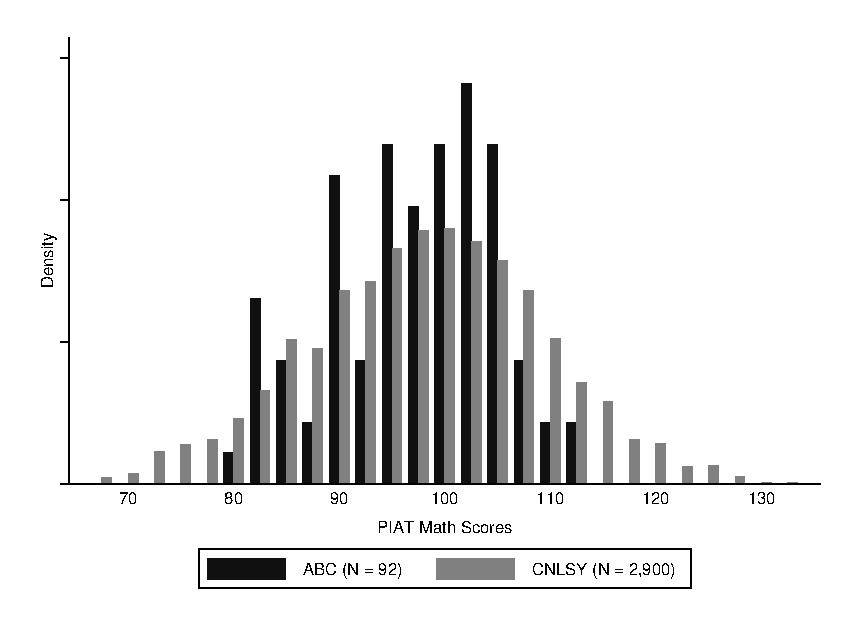
\includegraphics[width=\textwidth]{AppOutput/Methodology/support_math.eps}
	\end{subfigure}
	
	\begin{subfigure}[h]{0.8\textwidth}
	\centering
	\caption{Mother's Years of Education} \label{fig:support_meduc}
	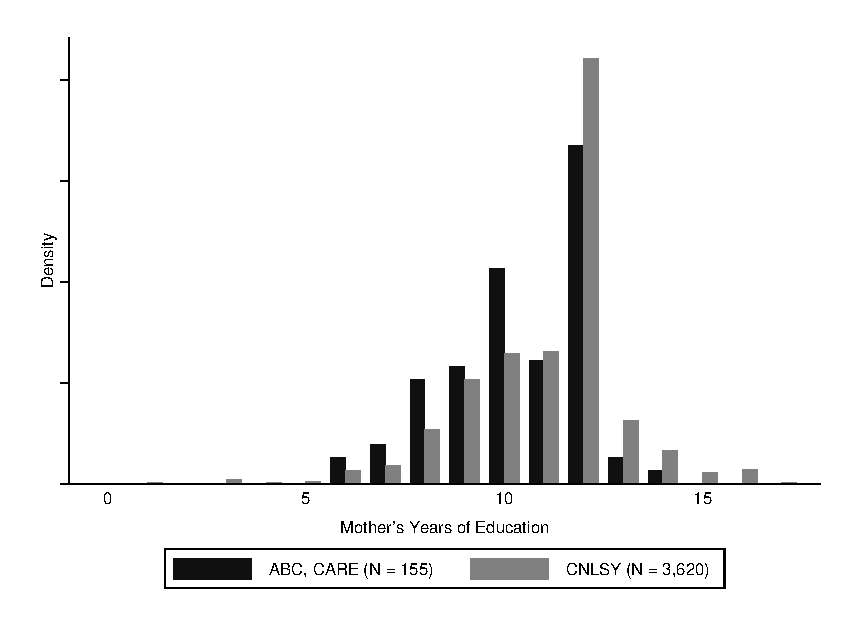
\includegraphics[width=\textwidth]{AppOutput/Methodology/support_momed.eps}
	\end{subfigure}
	
	\floatfoot{
	\footnotesize
	\noindent Note: These graphs display the support of ABC, PSID, NLSY79, and CNLSY
	for variables we use to project future labor income. PIAT math
	scores are averaged over ages 5--7.
	}
\end{figure}

\begin{figure}[H]
		\ContinuedFloat
	\begin{subfigure}[h]{0.8\textwidth}
	\centering
	\caption{Subject's Years of Education} \label{fig:support_educ}
	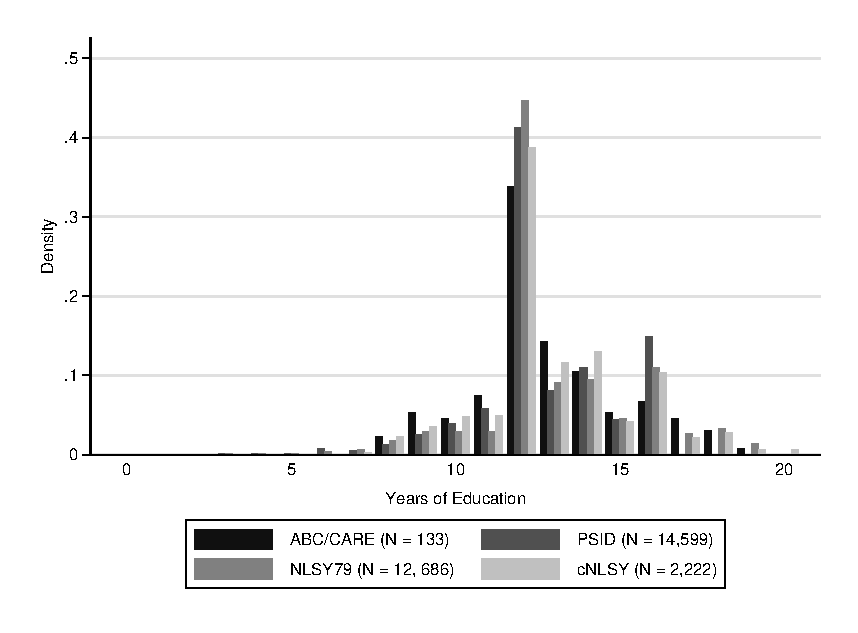
\includegraphics[width=\textwidth]{AppOutput/Methodology/support_educ.eps}
	\end{subfigure}
	
	\begin{subfigure}[h]{0.8\textwidth}
	\centering
	\caption{Income at Age 21} \label{fig:support_inc21}
	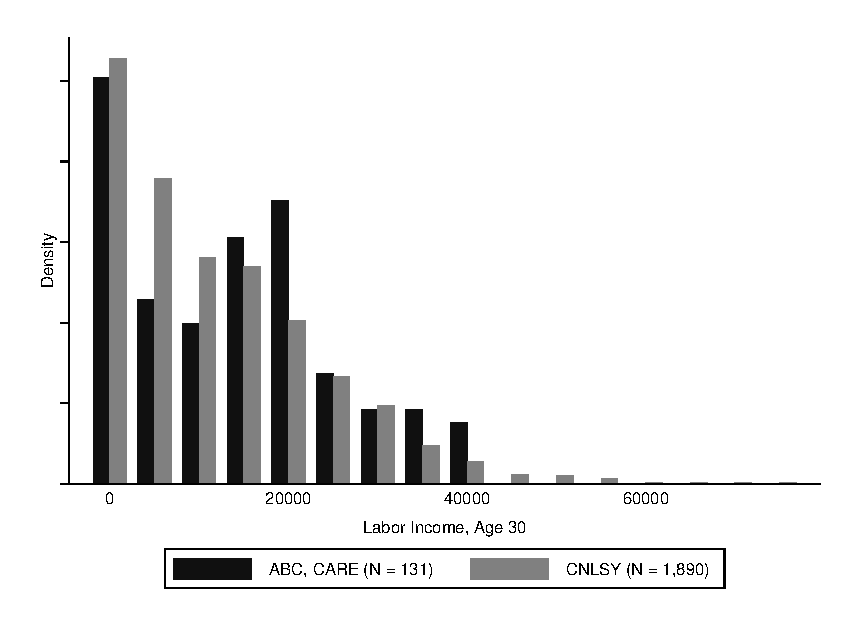
\includegraphics[width=\textwidth]{AppOutput/Methodology/support_inc21.eps}
	\end{subfigure}
	
\end{figure}

\begin{figure}[H]
	\ContinuedFloat
	
	\begin{subfigure}[h]{0.8\textwidth}
	\centering
	\caption{Income at Age 30} \label{fig:support_inc30}
	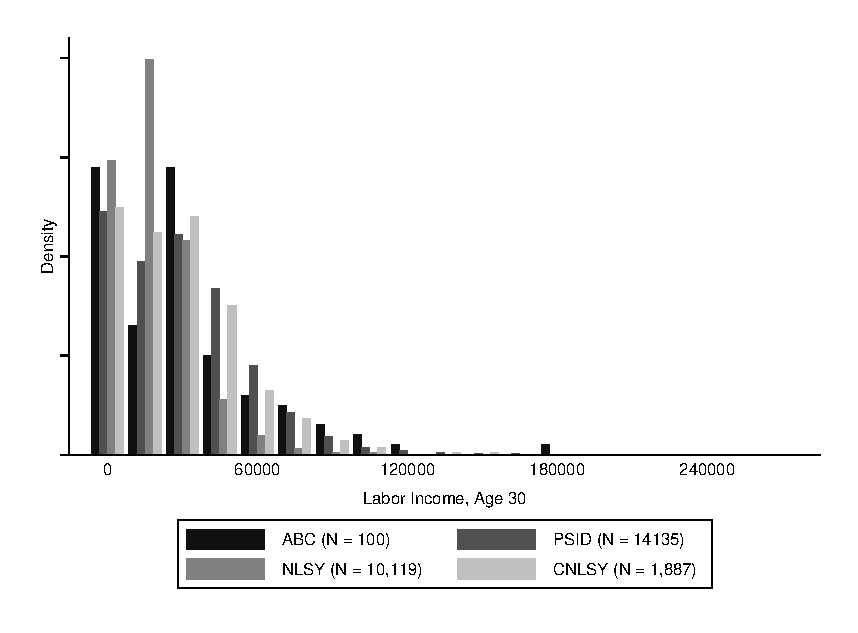
\includegraphics[width=\textwidth]{AppOutput/Methodology/support_inc30.eps}
	\end{subfigure}

	
	\begin{subfigure}[h]{0.8\textwidth}
	\centering
	\caption{Body Mass Index, Age 34} \label{fig:support_bmi}
	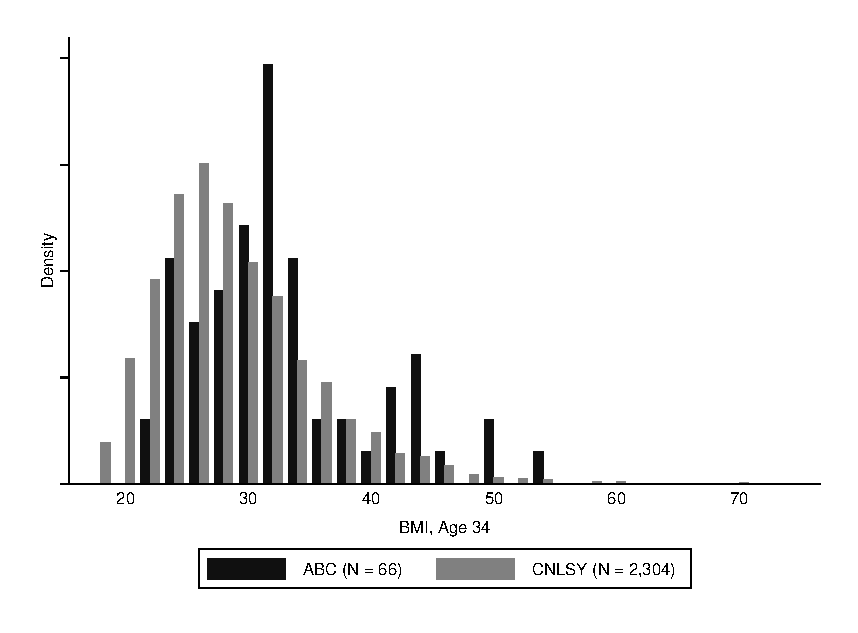
\includegraphics[width=\textwidth]{AppOutput/Methodology/support_bmi.eps}
	\end{subfigure}
	
\end{figure}

\subsubsection{Testing Assumption~\ref{ass:exog}: Exogeneity} \label{app:endogeneity}

\noindent The following framework help us to test both Assumptions~\ref{ass:exog} and \ref{ass:summary}. We provide this framework and test Assumption~\ref{ass:exog} in this section of the appendix, and test Assumption~\ref{ass:summary} in the next section.\\

\noindent Define an outcome vector as

\begin{align}
\bm{Y}_{k,a} &= \bm{X}^d_{k,a} \bm{\gamma} + \bm{\varepsilon}^d_a  &(a) \nonumber
\end{align}

\noindent with an associated measurement system

\begin{align}  \label{eq:sa-msystemmain}
\bm{\varepsilon}_{a}^d &=\bm{\beta}^d \bm{\theta}_{a}^d + \bm{\omega}_{a}^d  &(b) \nonumber \\
\bm{M}_{a}^d &= \bm{\lambda}^d \bm{\theta}_{a}^d + \bm{\upsilon}_a^d,  &(c)
\end{align}


\noindent where $\bm{\theta}^d \independent \bm{\upsilon}_{a}^d, \bm{\omega}_{a}^d$ and $\bm{\upsilon}_{a}^d \independent \bm{\omega}_{a}^d$ for all $a \in \{0, \ldots, A \}, \; d \in \{0,1\}$. We use predictors in these equations. For sake of simplicity, we omit an explicit representation of them here.\\

\noindent When the auxiliary measurement system $\bm{M}_{a}^d $ consists of at least three measures, we are able to identify the vectors of coefficients characterizing this system, $\bm{\lambda}^d, \bm{\beta}^d$, as well as the respective covariance matrices, $\bm{\Sigma}_{\bm{\theta}_{a}^d}, \bm{\Sigma}_{\bm{\upsilon}_{a}^d}, \bm{\Sigma}_{\bm{\omega}_{a}^d}$, and use the method of \citet{Bartlett_1938_Nature} to obtain an estimate of $\bm{\theta}_{a}^d$ \citep{Heckman_Pinto_etal_2013_PerryFactor}. Identifying and estimating the elements in System \eqref{eq:sa-msystemmain} helps two purposes: (i) propose a test of Assumption~\ref{ass:exog}; and (ii) use estimates of $\bm{\theta}_{a}^d$ as control functions when testing Assumption~\ref{ass:summary} in the next appendix, i.e. use these estimates to ``control'' for endogeneity.\\

\noindent We start by providing estimates for the elements in System~\eqref{eq:sa-msystemmain} in the experimental sample. We assume that $\bm{\theta}_{a}^d$ has two dimensions (one representing cognitive skill, $c$, and another representing non-cognitive skill, $n$). We assume dedicated measures for these skills at one time period. Put simply, we have two independent systems, one to measure $\bm{\theta}_{c}^d$ and one to measure $\bm{\theta}_{n}^d$, where $\bm{\theta}_{a}^d: = \left[ \bm{\theta}_{c}^d, \bm{\theta}_{n}^d \right]$. Further, we assume a common measurement system for the treatment and control groups (this is a sensible assumption shown to be true in the Perry data; see \citealp{Heckman_Pinto_etal_2013_PerryFactor}). This assumption implies that $\bm{\lambda}^d, \bm{\beta}^d$, as well as $\bm{\Sigma}_{\bm{\theta}_{a}^d}, \bm{\Sigma}_{\bm{\upsilon}_{a}^d}$ are the same whether $d = 0$ or $d = 1$.\\

\noindent We use a set of IQ measures from ages 2 to 8 to obtain an estimate of $\bm{\theta}_{c}^d$ and a set of measures of somatization, hostility, depression, and mental health all at age 21 to measure to estimate $\bm{\theta}_{n}^d$.\footnote{For definitions and treatment effects on these variables see Appendix~\ref{appendix:results}.} Figure~\ref{figure:factorsm} shows our estimates by treatment status.\\

\begin{figure}[!htbp]
\centering
\caption{Estimates of Cognitive ($\theta_{c}^d$) and Non-cognitive Skills ($\theta_{n}^d$)}\label{figure:factorsm}
\begin{subfigure}[h]{0.5\textwidth}
		\centering
		\caption{Cognitive} \label{fig:c}
		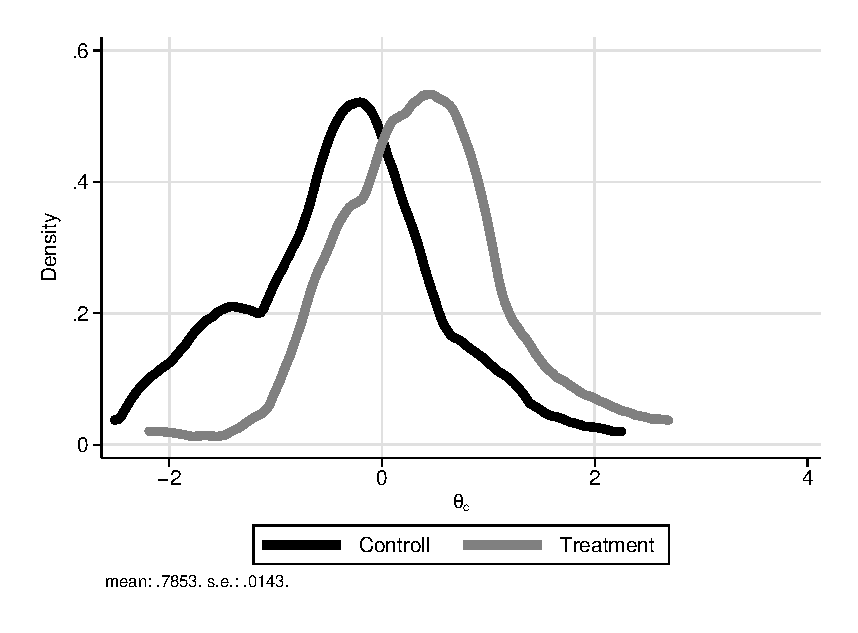
\includegraphics[width=\textwidth]{output/abccare_cfactor.eps}
\end{subfigure}%
\begin{subfigure}[h]{0.5\textwidth}
	\centering
	\caption{Non-cognitive} \label{fig:n}
		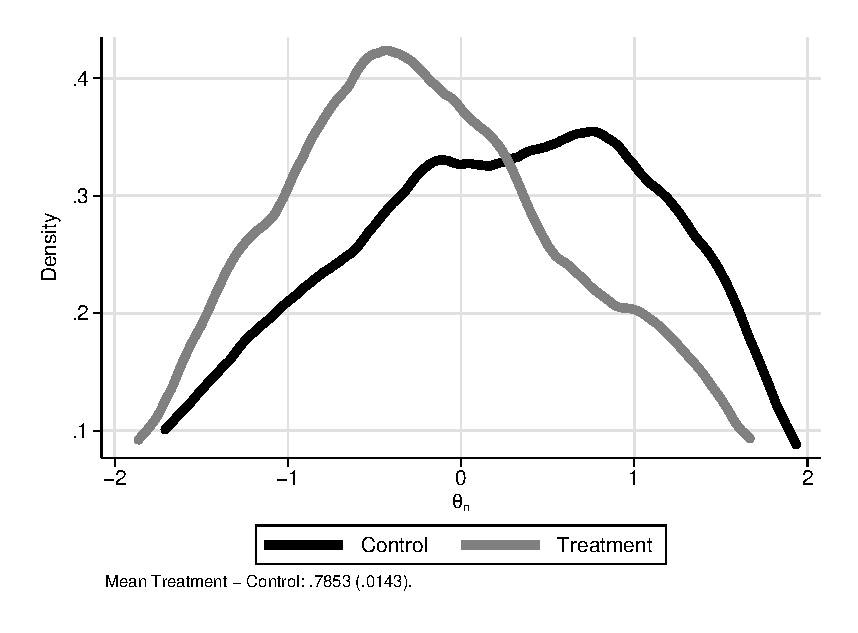
\includegraphics[width=\textwidth]{output/abccare_nfactor.eps}
\end{subfigure}
\footnotesize \justify
Note: Panel (a) displays a factor score estimated based on the measurement system in \eqref{eq:sa-msystemmain} and measures of IQ at ages 2, 3, 4, 5, 7, and 8 (cognitive skill). Panel (b) displays an analogous set of graphs for measures of somatization, hostility, depression, and mental health at age 21 (non-cognitive skill). Both measures of skills are standardized to a mean of $0$ and a standard deviation of $1$. ``Less'' in the factor measuring non-cognitive skills is ``positive'' given the measures we rely on to construct it. The mean difference between treatment and control is displayed below each panel, with standard error in parentheses. Standard errors are based on the empirical bootstrap distribution.
\end{figure}

\noindent We can also estimates $\bm{\theta}_{a}^d$ in the auxiliary sample. For want of data to approximate $\bm{\theta}_{c}, \bm{\theta}_{n}$ in PSID and NLSY79, we use the CNLSY in this appendix. Our measurement system for $\bm{\theta}_{c}$ consists of reading and comprehension PIAT scores as well as by the Peabody Picture Vocabulary Test (PPVT). Our measurement system for $\bm{\theta}_{n}$ is based on six scales of the Behavior Problems Index (e.g., anxiety, dependency, social behavior).\\

\noindent Once these estimates are available, we can test Assumption~\ref{ass:exog} in the experimental and auxiliary samples. The test consists of the following. Let $\bm{\gamma}^E$ be the parameter associated to $\bm{X}^d_{k,a}$ in Equation (a) in System~\eqref{eq:sa-msystemmain} when not accounting for $\bm{\theta}_{a}^d$. Similarly, let $\bm{\gamma}^I$ be the parameter associated with $\bm{X}^d_{k,a}$ in Equation (a) in System~\eqref{eq:sa-msystemmain} when accounting for $\bm{\theta}_{a}^d$. Under the null hypotheses, Assumption~\ref{ass:exog} holds and $\bm{\theta}_{a}^d$ is an irrelevant predictor in Equation (a) in System~\eqref{eq:sa-msystemmain}. This makes the OLS estimate of $\bm{\gamma}^E$ inconsistent. If the null hypotheses are false, $\bm{X}^d_{k,a}$ and $\varepsilon_{a}^d$ are not independent, $\bm{\gamma}^I$ is consistent and $\bm{\gamma}^E$ is not. We test the null hypothesis by asking if the elements in $\bm{\theta}_{a}^d$ are relevant predictors of a set of outcomes at age 30, so that we can perform the tests both the experimental and the auxiliary samples. We contrast specifications with and without including estimates of $\bm{\theta}_{a}^d$, and report the $F$-statistic corresponding to this comparison. This is a version of a Durbin-Wu-Hausman test \citep[see][]{Durbin_1954_RISI,Wu_1973_Econometrica,Hausman_1978_Econometrica}. Tables~\ref{table:endoginc} to \ref{table:trincome} present the results. In most cases, we are not able to reject the null hypothesis that Assumption~\ref{ass:exog} holds.\\


\begin{sidewaystable}[H]
\begin{threeparttable}
\caption{Prediction of Labor Income at Age 30 Accounting for $\bm{B}_k$ and $\bm{\theta}, \bm{X}_{k,a}$, ABC/CARE Control Group}
\label{table:endoginc}
\centering
\footnotesize
\begin{tabular}{lcccccccc} \toprule
 & (1) & (2) & (3) & (4) & (5) & (6) & (7) & (8) \\
 & Estimate & $p$-value & Estimate & $p$-value  & Estimate & $p$-value  & Estimate & $p$-value  \\ \midrule 
Mother's Education &     1,599.57 &         0.17 &       867.41 &         0.34 &      -769.20 &         0.68 &      -580.88 &         0.62 \\  
PIAT (5-7) &            . &            . &            . &            . &        45.98 &         0.41 &       423.44 &         0.20 \\  
Education (30) &            . &            . &            . &            . &     3,415.53 &         0.03 &     4,505.94 &         0.04 \\  
Labor Income (21) &            . &            . &            . &            . &         0.69 &         0.02 &         0.97 &         0.03 \\  
Cognitive &            . &            . &       758.28 &         0.43 &            . &            . &    -8,009.28 &         0.93 \\  
Non Cognitive &            . &            . &      -342.62 &         0.52 &            . &            . &     7,275.49 &         0.09 \\  
Constant &    10,239.82 &         0.28 &    16,530.50 &         0.22 &   -23,140.28 &         0.80 &   -80,679.09 &         0.96 \\  \\ \midrule
R2 &         \multicolumn{2}{c}{0.03} &              \multicolumn{2}{c}{0.07} &             \multicolumn{2}{c}{0.30} &               \multicolumn{2}{c}{0.40}  \\  
Observations &         \multicolumn{2}{c}{66} &          \multicolumn{2}{c}{51} &              \multicolumn{2}{c}{65} &             \multicolumn{2}{c}{63}  \\  \\ \midrule
$F$-stat: exclude Cognitive, Non-Cognitive &              \multicolumn{4}{c}{1.70} &               \multicolumn{4}{c}{4.14}  \\  
$p$-value  &         \multicolumn{4}{c}{0.45} &                   \multicolumn{4}{c}{0.09} \\      \bottomrule \end{tabular}


\begin{tablenotes}
\footnotesize
\item $F$-stat: exclude Cognitive and Non-Cognitive: $F$-statistic contrasting the specifications in columns (1) and (3) and (5) and (7), respectively.\\
\item Note: Prediction of labor income at age 30 based on the variables listed in the row. Empty cells indicate that the variable was not used in the prediction. For each coefficient we provide point estimate and $p$-value for the treatment and control groups and a test for the treatment-control difference. $\hat{\bm{\theta}}_{c}$: factor score estimated based on the measurement system in \eqref{eq:sa-msystemmain} and measures of IQ at ages 2, 3, 4, 5, 7, and 8 (cognitive skill). $\hat{\bm{\theta}}_{n}$: factor score estimated based on the measurement system in \eqref{eq:sa-msystemmain} and measures of somatization, hostility, depression, and a global mental health index at age 21 (non-cognitive skill). Both measures of skills are standardized to a mean of $0$ and a standard deviation of $1$. Inference is based on the empirical bootstrap distribution. If the estimates for the constant terms are in the ten or hundred thousands, we report a figure that has been rounded to the thousands.
\end{tablenotes}
\end{threeparttable}
\end{sidewaystable}

\begin{sidewaystable}[H]
\begin{threeparttable}
\caption{Prediction of Labor Income at Age 30 Accounting for $\bm{B}_k$ and $\bm{\theta}, \bm{X}_{k,a}$, ABC/CARE Treatment Group}
\centering
\footnotesize
\begin{tabular}{lcccccccc} \toprule
 & (1) & (2) & (3) & (4) & (5) & (6) & (7) & (8) \\
 & Estimate & $p$-value & Estimate & $p$-value  & Estimate & $p$-value  & Estimate & $p$-value  \\ \midrule 
Mother's Education &     3,134.16 &         0.23 &     2,600.34 &         0.35 &     2,913.44 &         0.28 &     5,835.67 &         0.22 \\  
PIAT (5-7) &            . &            . &            . &            . &      -263.29 &         0.66 &      -871.06 &         0.76 \\  
Education (30) &            . &            . &            . &            . &    11,600.24 &         0.00 &    13,069.48 &         0.00 \\  
Labor Income (21) &            . &            . &            . &            . &        -0.18 &         0.64 &        -0.62 &         0.75 \\  
Cognitive &            . &            . &     2,766.35 &         0.40 &            . &            . &     4,828.93 &         0.34 \\  
Non Cognitive &            . &            . &     7,600.33 &         0.18 &            . &            . &     6,223.32 &         0.19 \\  
Constant &     3,900.73 &         0.47 &    10,553.93 &         0.42 &  -122,709.85 &         0.91 &  -109,410.81 &         0.76 \\  \\ \midrule
$R^2$ &         \multicolumn{2}{c}{0.02} &          \multicolumn{2}{c}{0.10} &          \multicolumn{2}{c}{0.26} &             \multicolumn{2}{c}{0.33} \\ 
Observations &         \multicolumn{2}{c}{64} &         \multicolumn{2}{c}{49} &                \multicolumn{2}{c}{65} &       \multicolumn{2}{c}{63}  \\   \\ \midrule
$F$-stat: exclude Cognitive, Non-Cognitive &             \multicolumn{4}{c}{3.13} &              \multicolumn{4}{c}{2.14}  \\  
$p$-value &                 \multicolumn{4}{c}{0.27} &                   \multicolumn{4}{c}{0.27}  \\    \bottomrule \end{tabular}


\begin{tablenotes}
\footnotesize
\item $F$-stat: exclude Cognitive and Non-Cognitive: $F$-statistic contrasting the specifications in columns (1) and (3) and (5) and (7), respectively.\\
\item Note: Prediction of labor income at age 30 based on the variables listed in the row. Empty cells indicate that the variable was not used in the prediction. For each coefficient we provide point estimate and $p$-value for the treatment and control groups and a test for the treatment-control difference. $\hat{\bm{\theta}}_{c}$: factor score estimated based on the measurement system in \eqref{eq:sa-msystemmain} and measures of IQ at ages 2, 3, 4, 5, 7, and 8 (cognitive skill). $\hat{\bm{\theta}}_{n}$: factor score estimated based on the measurement system in \eqref{eq:sa-msystemmain} and measures of somatization, hostility, depression, and a global mental health index at age 21 (non-cognitive skill). Both measures of skills are standardized to a mean of $0$ and a standard deviation of $1$. Inference is based on the empirical bootstrap distribution. If the estimates for the constant terms are in the ten or hundred thousands, we report a figure that has been rounded to the thousands.
\end{tablenotes}
\end{threeparttable}
\end{sidewaystable}

\begin{sidewaystable}[H]
\begin{threeparttable}
\caption{Prediction of Labor Income at Age 30 Accounting for $\bm{B}_k$ and $\bm{\theta}, \bm{X}_{k,a}$, ABC/CARE Control and Treatment Groups}
\centering
\footnotesize
\begin{tabular}{lcccccccc} \toprule
 & (1) & (2) & (3) & (4) & (5) & (6) & (7) & (8) \\
 & Estimate & $p$-value & Estimate & $p$-value  & Estimate & $p$-value  & Estimate & $p$-value  \\ \midrule 
Mother's Education &     2,668.48 &         0.12 &     2,200.35 &         0.25 &       794.11 &         0.36 &     1,724.88 &         0.31 \\  
PIAT (5-7) &            . &            . &            . &            . &      -126.19 &         0.67 &      -400.57 &         0.72 \\  
Education (30) &            . &            . &            . &            . &     8,601.33 &         0.00 &     9,706.02 &         0.00 \\  
Labor Income (21) &            . &            . &            . &            . &         0.14 &         0.37 &         0.21 &         0.37 \\  
Cognitive &            . &            . &     4,260.39 &         0.16 &            . &            . &     1,427.18 &         0.44 \\  
Non Cognitive &            . &            . &     2,899.66 &         0.25 &            . &            . &     7,557.01 &         0.05 \\  
Constant &     4,443.37 &         0.41 &     9,166.30 &         0.38 &   -78,053.28 &         0.95 &   -75,621.84 &         0.87 \\  \\ \midrule
$R^2$ &         \multicolumn{2}{c}{0.02} &          \multicolumn{2}{c}{0.04} &             \multicolumn{2}{c}{0.20} &                 \multicolumn{2}{c}{0.25}  \\  
Observations &        \multicolumn{2}{c}{132} &        \multicolumn{2}{c}{100} &     \multicolumn{2}{c}{130} &         \multicolumn{2}{c}{133}  \\  \\ \midrule
$F$-stat: exclude Cognitive, Non-Cognitive  &             \multicolumn{4}{c}{2.07} &               \multicolumn{4}{c}{2.92}  \\  
$p$-value &                \multicolumn{4}{c}{0.31} &               \multicolumn{4}{c}{0.19}   \\  \bottomrule \end{tabular}
\begin{tablenotes}
\footnotesize
\item $F$-stat: exclude Cognitive and Non-Cognitive: $F$-statistic contrasting the specifications in columns (1) and (3) and (5) and (7), respectively.\\
\item Note: Prediction of labor income at age 30 based on the variables listed in the row. Empty cells indicate that the variable was not used in the prediction. For each coefficient we provide point estimate and $p$-value for the treatment and control groups and a test for the treatment-control difference. $\hat{\bm{\theta}}_{c}$: factor score estimated based on the measurement system in \eqref{eq:sa-msystemmain} and measures of IQ at ages 2, 3, 4, 5, 7, and 8 (cognitive skill). $\hat{\bm{\theta}}_{n}$: factor score estimated based on the measurement system in \eqref{eq:sa-msystemmain} and measures of somatization, hostility, depression, and a global mental health index at age 21 (non-cognitive skill). Both measures of skills are standardized to a mean of $0$ and a standard deviation of $1$. Inference is based on the empirical bootstrap distribution. If the estimates for the constant terms are in the ten or hundred thousands, we report a figure that has been rounded to the thousands.
\end{tablenotes}
\end{threeparttable}
\end{sidewaystable}

\begin{sidewaystable}[H]
\begin{threeparttable}
\caption{Prediction of Labor Income at Age 30 Accounting for $\bm{B}_k$ and $\bm{\theta}, \bm{X}_{k,a}$, CNLSY}
\centering
\footnotesize
\begin{tabular}{lcccccccc} \toprule
 & (1) & (2) & (3) & (4) & (5) & (6) & (7) & (8) \\
 & Estimate & $p$-value & Estimate & $p$-value  & Estimate & $p$-value  & Estimate & $p$-value  \\ \midrule 
Mother's Education &     2,317.52 &         0.00 &     2,262.79 &         0.00 &       316.78 &         0.23 &       379.54 &         0.32 \\  
PIAT (5-7) &            . &            . &            . &            . &       263.98 &         0.00 &       471.53 &         0.00 \\  
Education (30) &            . &            . &            . &            . &     3,647.75 &         0.00 &     4,351.32 &         0.00 \\  
Labor Income (21) &            . &            . &            . &            . &         0.68 &         0.00 &         0.79 &         0.00 \\  
Cognitive &            . &            . &     2,680.61 &         0.13 &            . &            . &    -4,541.18 &         0.95 \\  
Non Cognitive &            . &            . &    -3,584.83 &         0.99 &            . &            . &    -1,352.32 &         0.79 \\  
Constant &     2,523.10 &         0.25 &     3,699.61 &         0.37 &   -56,008.30 &         1.00 &   -86,767.50 &         1.00 \\ \\ \midrule
$R^2$ &         \multicolumn{2}{c}{0.03} &              \multicolumn{2}{c}{0.06} &               \multicolumn{2}{c}{0.21} &                \multicolumn{2}{c}{0.34}  \\  
Observations &       \multicolumn{2}{c}{1,885} &            \multicolumn{2}{c}{370} &           \multicolumn{2}{c}{1,885} &          \multicolumn{2}{c}{1,883}   \\  \\ \midrule
$F$-stat: exclude Cognitive, Non-Cognitive &                      \multicolumn{4}{c}{1.28} &                      \multicolumn{4}{c}{4.93}   \\  
$p$-value &             \multicolumn{4}{c}{0.44} &                  \multicolumn{4}{c}{0.44}  \\    \bottomrule \end{tabular}

\begin{tablenotes}
\footnotesize
\item $F$-stat: exclude Cognitive and Non-Cognitive: $F$-statistic contrasting the specifications in columns (1) and (3) and (5) and (7), respectively.\\
\item Note: Prediction of labor income at age 30 based on the variables listed in the row. Empty cells indicate that the variable was not used in the prediction. For each coefficient we provide point estimate and $p$-value for the treatment and control groups and a test for the treatment-control difference. $\hat{\bm{\theta}}_{c}$: factor score estimated based on the measurement system in \eqref{eq:sa-msystemmain} and measures of reading and comprehension of the PIAT, as weel as the Peabody Picture Vocabulary Test (PPVT) (cognitive skill). $\hat{\bm{\theta}}_{n}$: factor score estimated based on the measurement system in \eqref{eq:sa-msystemmain} and six scales of the Behavior Problems Index (e.g., anxiety, dependency, social behavior) (non-cognitive skill). Both measures of skills are standardized to a mean of $0$ and a standard deviation of $1$. Inference is based on the empirical bootstrap distribution. If the estimates for the constant terms are in the ten or hundred thousands, we report a figure that has been rounded to the thousands.
\end{tablenotes}
\end{threeparttable}
\end{sidewaystable}

\begin{sidewaystable}[H]
\begin{threeparttable}
\caption{Prediction of Transfer Income at Age 30 Accounting for $\bm{B}_k$ and $\bm{\theta}, \bm{X}_{k,a}$, ABC/CARE Control Group}
\label{table:endoginc}
\centering
\footnotesize
\begin{tabular}{lcccccccc} \toprule
 & (1) & (2) & (3) & (4) & (5) & (6) & (7) & (8) \\
 & Estimate & $p$-value & Estimate & $p$-value  & Estimate & $p$-value  & Estimate & $p$-value  \\ \midrule 
Mother's Education &      -413.76 &         0.78 &      -406.14 &         0.69 &        48.75 &         0.49 &        51.97 &         0.47 \\  
PIAT (5-7) &            . &            . &            . &            . &        27.10 &         0.29 &      -101.93 &         0.77 \\  
Education (30) &            . &            . &            . &            . &      -684.75 &         0.99 &      -693.44 &         0.91 \\  
Labor Income (21) &            . &            . &            . &            . &        -0.14 &         0.99 &        -0.15 &         0.93 \\  
Cognitive &            . &            . &      -348.53 &         0.69 &            . &            . &     1,696.96 &         0.13 \\  
Non Cognitive &            . &            . &     1,622.92 &         0.05 &            . &            . &       887.17 &         0.19 \\  
Constant &     6,664.39 &         0.11 &     6,614.39 &         0.18 &     9,942.56 &         0.18 &    22,736.59 &         0.10 \\  \\ \midrule 
$F$-stat &          \multicolumn{2}{c}{1.93} &             \multicolumn{2}{c}{2.96} &            \multicolumn{2}{c}{3.53} &              \multicolumn{2}{c}{2.68}   \\  
$p$-value &          \multicolumn{2}{c}{0.34} &             \multicolumn{2}{c}{0.15} &            \multicolumn{2}{c}{0.21} &              \multicolumn{2}{c}{0.27}   \\  
$R^2$ &          \multicolumn{2}{c}{0.04} &             \multicolumn{2}{c}{0.15} &            \multicolumn{2}{c}{0.21} &              \multicolumn{2}{c}{0.27}   \\  
Observations &         \multicolumn{2}{c}{68} &                 \multicolumn{2}{c}{52} &               \multicolumn{2}{c}{70}  &                \multicolumn{2}{c}{70}   \\  \\ \midrule
$F$-stat: exclude Cognitive, Non-Cognitive  &                 \multicolumn{4}{c}{3.38} &              \multicolumn{4}{c}{2.42}  \\  
$p$-value &                \multicolumn{4}{c}{0.19} &               \multicolumn{4}{c}{0.27}  \\      \bottomrule \end{tabular}
\begin{tablenotes}
\footnotesize
\item $F$-stat: exclude Cognitive and Non-Cognitive: $F$-statistic contrasting the specifications in columns (1) and (3) and (5) and (7), respectively.\\
\item Note: Prediction of transfer income at age 30 based on the variables listed in the row. Empty cells indicate that the variable was not used in the prediction. For each coefficient we provide point estimate and $p$-value for the treatment and control groups and a test for the treatment-control difference. $\hat{\bm{\theta}}_{c}$: factor score estimated based on the measurement system in \eqref{eq:sa-msystemmain} and measures of IQ at ages 2, 3, 4, 5, 7, and 8 (cognitive skill). $\hat{\bm{\theta}}_{n}$: factor score estimated based on the measurement system in \eqref{eq:sa-msystemmain} and measures of somatization, hostility, depression, and a global mental health index at age 21 (non-cognitive skill). Both measures of skills are standardized to a mean of $0$ and a standard deviation of $1$. Inference is based on the empirical bootstrap distribution. If the estimates for the constant terms are in the ten or hundred thousands, we report a figure that has been rounded to the thousands.
\end{tablenotes}
\end{threeparttable}
\end{sidewaystable}

\begin{sidewaystable}[H]
\begin{threeparttable}
\caption{Prediction of Transfer Income at Age 30 Accounting for $\bm{B}_k$ and $\bm{\theta}, \bm{X}_{k,a}$, ABC/CARE Treatment Group}
\centering
\footnotesize
\begin{tabular}{lcccccccc} \toprule
 & (1) & (2) & (3) & (4) & (5) & (6) & (7) & (8) \\
 & Estimate & $p$-value & Estimate & $p$-value  & Estimate & $p$-value  & Estimate & $p$-value  \\ \midrule 
Mother'sEducation &      -212.39 &         0.75 &      -336.44 &         0.81 &      -199.39 &         0.74 &      -302.60 &         0.79 \\  
PIAT(5-7) &            . &            . &            . &            . &       -46.36 &         0.86 &       -22.41 &         0.65 \\  
Education(30) &            . &            . &            . &            . &       -35.62 &         0.56 &       -72.66 &         0.59 \\  
LaborIncome(21) &            . &            . &            . &            . &        -0.05 &         0.94 &        -0.05 &         0.90 \\  
Cognitive &            . &            . &      -421.59 &         0.75 &            . &            . &      -273.48 &         0.62 \\  
Non Cognitive &            . &            . &      -825.26 &         0.95 &            . &            . &      -987.11 &         0.98 \\  
Constant &     3,348.22 &         0.16 &     4,937.75 &         0.14 &     9,041.98 &         0.09 &     8,432.47 &         0.18 \\  \\ \midrule
$R^2$  &          \multicolumn{2}{c}{0.03} &            \multicolumn{2}{c}{0.15} &                  \multicolumn{2}{c}{0.13} &               \multicolumn{2}{c}{0.25}  \\  
Observations &        \multicolumn{2}{c}{63} &               \multicolumn{2}{c}{49}  &             \multicolumn{2}{c}{65}  &         \multicolumn{2}{c}{63}  \\   \\ \midrule
$F$-stat: exclude Cognitive, Non-Cognitive &                    \multicolumn{4}{c}{4.15} &                   \multicolumn{4}{c}{2.90}  \\  
$p$-value &              \multicolumn{4}{c}{0.28} &                    \multicolumn{4}{c}{0.28}  \\      \bottomrule \end{tabular}
\begin{tablenotes}
\footnotesize
\item $F$-stat: exclude Cognitive and Non-Cognitive: $F$-statistic contrasting the specifications in columns (1) and (3) and (5) and (7), respectively.\\
\item Note: Prediction of transfer income at age 30 based on the variables listed in the row. Empty cells indicate that the variable was not used in the prediction. For each coefficient we provide point estimate and $p$-value for the treatment and control groups and a test for the treatment-control difference. $\hat{\bm{\theta}}_{c}$: factor score estimated based on the measurement system in \eqref{eq:sa-msystemmain} and measures of IQ at ages 2, 3, 4, 5, 7, and 8 (cognitive skill). $\hat{\bm{\theta}}_{n}$: factor score estimated based on the measurement system in \eqref{eq:sa-msystemmain} and measures of somatization, hostility, depression, and a global mental health index at age 21 (non-cognitive skill). Both measures of skills are standardized to a mean of $0$ and a standard deviation of $1$. Inference is based on the empirical bootstrap distribution. If the estimates for the constant terms are in the ten or hundred thousands, we report a figure that has been rounded to the thousands.
\end{tablenotes}
\end{threeparttable}
\end{sidewaystable}

\begin{sidewaystable}[H]
\begin{threeparttable}
\caption{Prediction of Transfer Income at Age 30 Accounting for $\bm{B}_k$ and $\bm{\theta}, \bm{X}_{k,a}$, ABC/CARE Control and Treatment Groups}
\centering
\footnotesize
\begin{tabular}{lcccccccc} \toprule
 & (1) & (2) & (3) & (4) & (5) & (6) & (7) & (8) \\
 & Estimate & $p$-value & Estimate & $p$-value  & Estimate & $p$-value  & Estimate & $p$-value  \\ \midrule 
Mother's Education &      -299.72 &         0.81 &      -411.12 &         0.85 &      -135.23 &         0.62 &      -211.76 &         0.68 \\  
PIAT (5-7) &            . &            . &            . &            . &       -34.90 &         0.81 &       -66.99 &         0.80 \\  
Education (30) &            . &            . &            . &            . &      -430.88 &         0.96 &      -453.82 &         0.96 \\  
Labor Income (21) &            . &            . &            . &            . &        -0.09 &         1.00 &        -0.08 &         0.96 \\  
Cognitive &            . &            . &      -753.98 &         0.93 &            . &            . &       153.54 &         0.42 \\  
Non Cognitive &            . &            . &       631.74 &         0.17 &            . &            . &       264.49 &         0.34 \\  
Constant &     5,135.83 &         0.06 &     6,460.15 &         0.07 &    13,548.68 &         0.03 &    17,791.02 &         0.05 \\   \\ \midrule
$F$-stat &         \multicolumn{2}{c}{1.78} &         \multicolumn{2}{c}{3.04} &               \multicolumn{2}{c}{3.86} &            \multicolumn{2}{c}{2.75}  \\  
$p$-value &         \multicolumn{2}{c}{0.35} &         \multicolumn{2}{c}{0.12} &               \multicolumn{2}{c}{0.35} &            \multicolumn{2}{c}{0.09}  \\  
$R^2$ &         \multicolumn{2}{c}{0.02} &         \multicolumn{2}{c}{0.10} &               \multicolumn{2}{c}{0.15} &            \multicolumn{2}{c}{0.18}  \\  
Observations &       \multicolumn{2}{c}{133} &           \multicolumn{2}{c}{101} &         \multicolumn{2}{c}{135} &            \multicolumn{2}{c}{133}  \\  \\ \midrule
$F$-stat: exclude Cognitive, Non-Cognitive &              \multicolumn{4}{c}{3.38} &             \multicolumn{4}{c}{1.23}  \\  
$p$-value &            \multicolumn{4}{c}{0.17} &               \multicolumn{4}{c}{0.44}  \\   \bottomrule \end{tabular}


\begin{tablenotes}
\footnotesize
\item $F$-stat: exclude Cognitive and Non-Cognitive: $F$-statistic contrasting the specifications in columns (1) and (3) and (5) and (7), respectively.\\
\item Note: Prediction of transfer income at age 30 based on the variables listed in the row. Empty cells indicate that the variable was not used in the prediction. For each coefficient we provide point estimate and $p$-value for the treatment and control groups and a test for the treatment-control difference. $\hat{\bm{\theta}}_{c}$: factor score estimated based on the measurement system in \eqref{eq:sa-msystemmain} and measures of IQ at ages 2, 3, 4, 5, 7, and 8 (cognitive skill). $\hat{\bm{\theta}}_{n}$: factor score estimated based on the measurement system in \eqref{eq:sa-msystemmain} and measures of somatization, hostility, depression, and a global mental health index at age 21 (non-cognitive skill). Both measures of skills are standardized to a mean of $0$ and a standard deviation of $1$. Inference is based on the empirical bootstrap distribution. If the estimates for the constant terms are in the ten or hundred thousands, we report a figure that has been rounded to the thousands.
\end{tablenotes}
\end{threeparttable}
\end{sidewaystable}

\begin{sidewaystable}[H]
\begin{threeparttable}
\caption{Prediction of Transfer Income at Age 30 Accounting for $\bm{B}_k$ and $\bm{\theta}, \bm{X}_{k,a}$, CNLSY} \label{table:trincome}
\centering
\footnotesize
\begin{tabular}{lcccccccc} \toprule
 & (1) & (2) & (3) & (4) & (5) & (6) & (7) & (8) \\
 & Estimate & $p$-value & Estimate & $p$-value  & Estimate & $p$-value  & Estimate & $p$-value  \\ \midrule 
Mother'sEducation &      -457.46 &         0.56 &     8,259.13 &         0.04 &       985.13 &         0.41 &     9,344.69 &         0.02 \\  
PIAT(5-7) &            . &            . &            . &            . &      -273.46 &         0.64 &      -506.25 &         0.70 \\  
Education(30) &            . &            . &            . &            . &    -7,235.35 &         0.96 &    -5,622.52 &         0.84 \\  
LaborIncome(21) &            . &            . &            . &            . &         0.17 &         0.40 &        -0.96 &         0.98 \\  
Cognitive &            . &            . &    -8,525.66 &         0.83 &            . &            . &      -473.24 &         0.52 \\  
NonCognitive &            . &            . &    18,373.65 &         0.03 &            . &            . &     6,585.57 &         0.22 \\  
Constant &    34,777.07 &         0.14 &   -58,507.25 &         0.91 &   137,947.14 &         0.14 &    57,813.64 &         0.35 \\  \\ \midrule
$R^2$ &         \multicolumn{2}{c}{0.00} &               \multicolumn{2}{c}{0.02} &                \multicolumn{2}{c}{0.01} &             \multicolumn{2}{c}{0.05}   \\  
Observations &       \multicolumn{2}{c}{1,145} &              \multicolumn{2}{c}{244}  &       \multicolumn{2}{c}{1,145} &      \multicolumn{2}{c}{1,148}   \\  \\ \midrule
$F$-stat: exclude Cognitive, Non-Cognitive &                \multicolumn{4}{c}{1.86} &                 \multicolumn{4}{c}{1.03}   \\  
$p$-value  &                \multicolumn{4}{c}{0.23} &                \multicolumn{4}{c}{0.45}    \\  \bottomrule \end{tabular}


\begin{tablenotes}
\footnotesize
\item $F$-stat: exclude Cognitive and Non-Cognitive: $F$-statistic contrasting the specifications in columns (1) and (3) and (5) and (7), respectively.\\
\item Note: Prediction of transfer income at age 30 based on the variables listed in the row. Empty cells indicate that the variable was not used in the prediction. For each coefficient we provide point estimate and $p$-value for the treatment and control groups and a test for the treatment-control difference.$\hat{\bm{\theta}}_{c}$: factor score estimated based on the measurement system in \eqref{eq:sa-msystemmain} and measures of reading and comprehension of the PIAT, as weel as the Peabody Picture Vocabulary Test (PPVT) (cognitive skill). $\hat{\bm{\theta}}_{n}$: factor score estimated based on the measurement system in \eqref{eq:sa-msystemmain} and six scales of the Behavior Problems Index (e.g., anxiety, dependency, social behavior) (non-cognitive skill).  Both measures of skills are standardized to a mean of $0$ and a standard deviation of $1$. Inference is based on the empirical bootstrap distribution. If the estimates for the constant terms are in the ten or hundred thousands, we report a figure that has been rounded to the thousands.
\end{tablenotes}
\end{threeparttable}
\end{sidewaystable}

\subsubsection{Testing Assumption~\ref{ass:summary}: Structural Invariance} \label{app:invariance}

In this appendix, we use the framework in Appendix~\ref{app:endogeneity} to tests Assumption~\ref{ass:summary}. The tests are under the null hypothesis that Assumption~\ref{ass:exog} holds. In the main text we show that Assumption~\ref{ass:summary}, together with Assumption~\ref{ass:exog}, implies:

\begin{equation}\label{eq:invariancetestapp}
\mathbb{E} \left[ Y_{k,j,a}^d | \bm{X}_{k,a}^d  = \bm{x}, \bm{B}_k = \bm{b}, D = d \right] = \mathbb{E} \left[ Y_{k,j,a} | \bm{X}^d_{k,a}  = \bm{x}, \bm{B}_k = \bm{b} \right],
\end{equation}
for $a \in \{1,\dots,A\}$, $k \in \{e,n\}$, and $d \in \{0,1\}$.\\

\noindent A direct test of this hypothesis is to use the experimental sample and ask if once we account for a set of the variables in $\bm{X}_{k,a}$, $R$ (randomization to treatment assignment in ABC/CARE, which, as discussed in text, is equivalent to $D$) predicts the outcome of interest, conditional on $\bm{B}_k$. This tests if this specific set of $\bm{X}_{k,a}$ suffices to summarize the treatment generated by $R$. Under the null hypothesis, the coefficient associated to $R$ when predicting based on $\bm{B}_k$ and $\bm{X}_{k,a}$ is zero. We test this using the following predictors. Average Mathematics PIAT scores at ages 5 to 7, education at age 30, and labor income at age 21. That is, children who are offered treatment attend it. For a set of outcomes of interest, even beyond those that we predict, once we condition on $\bm{B}_k, \bm{X}_{k,a}, \bm{\theta}$, the coefficient associated with $R$ is not significant. We test this with and without accounting for endogeneity, as explained in Appendix~\ref{app:endogeneity}.\\

\begin{sidewaystable}[H]
\begin{threeparttable}
\caption{Prediction of High School Graduation at Age 30 Accounting for $R, \bm{B}_k, \bm{\theta},$ and $\bm{X}_{k,a}$ Pooled Sample, ABC/CARE}
\label{table:end2}
\centering
\scriptsize
\begin{tabular}{lcccccccc} \toprule
 & (1) & (2) & (3) & (4) & (5) & (6) & (7) & (8) \\ 
 & Estimate  & $p$-value  & Estimate  & $p$-value  & Estimate  & $p$-value  & Estimate  & $p$-value  \\  \midrule
$R$ &     0.130 &     0.040 &     0.106 &     0.170 &     0.019 &     0.415 &     0.019 &     0.425 \\  
Mother's Education &     0.093 &     0.000 &     0.081 &     0.000 &     0.051 &     0.000 &     0.043 &     0.050 \\  
PIAT (5-7) &         . &         . &         . &         . &    -0.005 &     0.910 &    -0.004 &     0.765 \\  
Education (30) &         . &         . &         . &         . &     0.119 &     0.000 &     0.124 &     0.000 \\  
Labor Income (21) &         . &         . &         . &         . &     0.000 &     0.005 &     0.000 &     0.010 \\  
Cognitive &         . &         . &     0.020 &     0.360 &         . &         . &    -0.038 &     0.740 \\  
Non Cognitive &         . &         . &    -0.027 &     0.720 &         . &         . &     0.011 &     0.395 \\  
Constant &    -0.410 &     0.985 &    -0.283 &     0.865 &    -1.082 &     1.000 &    -1.148 &     0.985 \\  \\ \midrule
$F$-stat &    \multicolumn{2}{c}{14.497} &          \multicolumn{2}{c}{5.819} &         \multicolumn{2}{c}{40.509} &           \multicolumn{2}{c}{25.147} \\  
$R^2$ &     \multicolumn{2}{c}{0.151} &          \multicolumn{2}{c}{0.143} &              \multicolumn{2}{c}{0.440} &          \multicolumn{2}{c}{0.434} \\  
Observations &   \multicolumn{2}{c}{134} &           \multicolumn{2}{c}{102} &          \multicolumn{2}{c}{135} &         \multicolumn{2}{c}{133} \\  \bottomrule \end{tabular}

\begin{tablenotes}
\footnotesize
\item Note: Prediction of high school graduation at age 30 based on the variables listed in the row. Empty cells indicate that the variable was not used in the prediction. For each coefficient we provide point estimate and $p$-value. $\hat{\bm{\theta}}_{c}$: factor score estimated based on the measurement system in \eqref{eq:sa-msystemmain} and PIAT sections that we do not use to predict (reading and comprehension) as well as by the Peabody Picture Vocabulary Test (PPVT) (cognitive skill). $\hat{\bm{\theta}}_{n}$: factor score estimated based on the measurement system in \eqref{eq:sa-msystemmain} and on six scales of the Behavior Problems Index (e.g., anxiety, dependency, social behavior). Inference is based on the empirical bootstrap distribution. If the estimates for the constant terms are in the ten or hundred thousands, we report a figure that has been rounded to the thousands.
\end{tablenotes}
\end{threeparttable}
\end{sidewaystable}

\begin{sidewaystable}[H]
\begin{threeparttable}
\caption{Prediction of High School Graduation at Age 30 Accounting for $R, \bm{B}_k, \bm{\theta},$ and $\bm{X}_{k,a}$ Female Sample, ABC/CARE}
\label{table:end2}
\centering
\scriptsize
\begin{tabular}{lcccccccc} \toprule
 & (1) & (2) & (3) & (4) & (5) & (6) & (7) & (8) \\ 
 & Estimate  & $p$-value  & Estimate  & $p$-value  & Estimate  & $p$-value  & Estimate  & $p$-value  \\  \midrule
$R$ &     0.196 &     0.010 &     0.091 &     0.250 &     0.031 &     0.385 &     0.037 &     0.425 \\  
Mother's Education &     0.077 &     0.000 &     0.062 &     0.050 &     0.036 &     0.055 &     0.023 &     0.170 \\  
PIAT (5-7) &         . &         . &         . &         . &    -0.008 &     0.860 &    -0.004 &     0.655 \\  
Education (30) &         . &         . &         . &         . &     0.093 &     0.000 &     0.102 &     0.005 \\  
Labor Income (21) &         . &         . &         . &         . &     0.000 &     0.000 &     0.000 &     0.000 \\  
Cognitive &         . &         . &     0.051 &     0.285 &         . &         . &    -0.073 &     0.775 \\  
Non Cognitive &         . &         . &    -0.076 &     0.895 &         . &         . &     0.051 &     0.200 \\  
Constant &    -0.266 &     0.800 &    -0.065 &     0.540 &    -0.444 &     0.790 &    -0.872 &     0.870 \\  \\ \midrule
$F$-stat &    \multicolumn{2}{c}{10.180} &     \multicolumn{2}{c}{5.545} &          \multicolumn{2}{c}{35.887} &          \multicolumn{2}{c}{31.753} \\  
$R^2$ &     \multicolumn{2}{c}{0.172} &         \multicolumn{2}{c}{0.197} &         \multicolumn{2}{c}{0.556} &           \multicolumn{2}{c}{0.612}  \\  
Observations &    \multicolumn{2}{c}{68} &         \multicolumn{2}{c}{53} &          \multicolumn{2}{c}{70} &          \multicolumn{2}{c}{70} \\  \bottomrule 
\end{tabular}


\begin{tablenotes}
\footnotesize
\item Note: Prediction of high school graduation at age 30 based on the variables listed in the row. Empty cells indicate that the variable was not used in the prediction. For each coefficient we provide point estimate and $p$-value. $\hat{\bm{\theta}}_{c}$: factor score estimated based on the measurement system in \eqref{eq:sa-msystemmain} and PIAT sections that we do not use to predict (reading and comprehension) as well as by the Peabody Picture Vocabulary Test (PPVT) (cognitive skill). $\hat{\bm{\theta}}_{n}$: factor score estimated based on the measurement system in \eqref{eq:sa-msystemmain} and on six scales of the Behavior Problems Index (e.g., anxiety, dependency, social behavior). Inference is based on the empirical bootstrap distribution. If the estimates for the constant terms are in the ten or hundred thousands, we report a figure that has been rounded to the thousands.
\end{tablenotes}
\end{threeparttable}
\end{sidewaystable}

\begin{sidewaystable}[H]
\begin{threeparttable}
\caption{Prediction of High School Graduation at Age 30 Accounting for $R, \bm{B}_k, \bm{\theta},$ and $\bm{X}_{k,a}$ Male Sample, ABC/CARE}
\label{table:end2}
\centering
\scriptsize
\begin{tabular}{lcccccccc} \toprule
 & (1) & (2) & (3) & (4) & (5) & (6) & (7) & (8) \\ 
 & Estimate  & $p$-value  & Estimate  & $p$-value  & Estimate  & $p$-value  & Estimate  & $p$-value  \\  \midrule
$R$ &     0.084 &     0.220 &     0.146 &     0.140 &     0.088 &     0.190 &     0.067 &     0.305 \\  
Mother's Education &     0.116 &     0.000 &     0.131 &     0.000 &     0.057 &     0.045 &     0.072 &     0.095 \\  
PIAT (5-7) &         . &         . &         . &         . &     0.000 &     0.470 &    -0.000 &     0.500 \\  
Education (30) &         . &         . &         . &         . &     0.152 &     0.000 &     0.156 &     0.000 \\  
Labor Income (21) &         . &         . &         . &         . &     0.000 &     0.170 &     0.000 &     0.440 \\  
Cognitive &         . &         . &    -0.023 &     0.645 &         . &         . &    -0.009 &     0.525 \\  
Non Cognitive &         . &         . &     0.051 &     0.195 &         . &         . &     0.004 &     0.475 \\  
Constant &    -0.636 &     0.970 &    -0.824 &     0.950 &    -2.092 &     1.000 &    -2.227 &     0.955 \\  \\ \hline
$F$-stat &    \multicolumn{2}{c}{11.144} &          \multicolumn{2}{c}{6.555} &           \multicolumn{2}{c}{17.009} &    \multicolumn{2}{c}{10.294}  \\  
$R^2$ &     \multicolumn{2}{c}{0.190} &            \multicolumn{2}{c}{0.215} &           \multicolumn{2}{c}{0.467} &     \multicolumn{2}{c}{0.460}  \\  
Observations &    \multicolumn{2}{c}{67} &           \multicolumn{2}{c}{49} &           \multicolumn{2}{c}{65} &   \multicolumn{2}{c}{70} \\  
\bottomrule \end{tabular}

\begin{tablenotes}
\footnotesize
\item Note: Prediction of high school graduation at age 30 based on the variables listed in the row. Empty cells indicate that the variable was not used in the prediction. For each coefficient we provide point estimate and $p$-value. $\hat{\bm{\theta}}_{c}$: factor score estimated based on the measurement system in \eqref{eq:sa-msystemmain} and PIAT sections that we do not use to predict (reading and comprehension) as well as by the Peabody Picture Vocabulary Test (PPVT) (cognitive skill). $\hat{\bm{\theta}}_{n}$: factor score estimated based on the measurement system in \eqref{eq:sa-msystemmain} and on six scales of the Behavior Problems Index (e.g., anxiety, dependency, social behavior). Inference is based on the empirical bootstrap distribution. If the estimates for the constant terms are in the ten or hundred thousands, we report a figure that has been rounded to the thousands.
\end{tablenotes}
\end{threeparttable}
\end{sidewaystable}


\begin{sidewaystable}[H]
\begin{threeparttable}
\caption{Prediction of Employment at Age 30 Accounting for $R, \bm{B}_k, \bm{\theta},$ and $\bm{X}_{k,a}$ Pooled Sample, ABC/CARE}
\label{table:end2}
\centering
\scriptsize
\begin{tabular}{lcccccccc} \toprule
 & (1) & (2) & (3) & (4) & (5) & (6) & (7) & (8) \\ 
 & Estimate  & $p$-value  & Estimate  & $p$-value  & Estimate  & $p$-value  & Estimate  & $p$-value  \\  \midrule
$R$ &     0.123 &     0.040 &     0.121 &     0.115 &    -0.008 &     0.550 &     0.057 &     0.265 \\  
Mother's Education &     0.033 &     0.060 &     0.017 &     0.230 &     0.031 &     0.150 &     0.029 &     0.155 \\  
PIAT (5-7) &         . &         . &         . &         . &     0.008 &     0.020 &     0.012 &     0.060 \\  
Education (30) &         . &         . &         . &         . &     0.046 &     0.005 &     0.026 &     0.080 \\  
Labor Income (21) &         . &         . &         . &         . &    -0.000 &     0.850 &    -0.000 &     0.875 \\  
Cognitive &         . &         . &     0.077 &     0.060 &         . &         . &    -0.016 &     0.595 \\  
Non Cognitive &         . &         . &     0.034 &     0.285 &         . &         . &     0.060 &     0.170 \\  
Constant &     0.361 &     0.075 &     0.530 &     0.020 &    -0.877 &     0.975 &    -0.966 &     0.895 \\  \\ \midrule
$F$-stat &     \multicolumn{2}{c}{3.903} &              \multicolumn{2}{c}{4.073} &              \multicolumn{2}{c}{5.239} &              \multicolumn{2}{c}{3.979}           \\  
$R^2$ &     \multicolumn{2}{c}{0.057} &              \multicolumn{2}{c}{0.124} &              \multicolumn{2}{c}{0.177} &              \multicolumn{2}{c}{0.229}           \\  
Observations &   \multicolumn{2}{c}{133} &            \multicolumn{2}{c}{101} &          \multicolumn{2}{c}{135} &            \multicolumn{2}{c}{133}           \\  \bottomrule \end{tabular}

\begin{tablenotes}
\footnotesize
\item Note: Prediction of employment at age 30 based on the variables listed in the row. Empty cells indicate that the variable was not used in the prediction. For each coefficient we provide point estimate and $p$-value. $\hat{\bm{\theta}}_{c}$: factor score estimated based on the measurement system in \eqref{eq:sa-msystemmain} and PIAT sections that we do not use to predict (reading and comprehension) as well as by the Peabody Picture Vocabulary Test (PPVT) (cognitive skill). $\hat{\bm{\theta}}_{n}$: factor score estimated based on the measurement system in \eqref{eq:sa-msystemmain} and on six scales of the Behavior Problems Index (e.g., anxiety, dependency, social behavior). Inference is based on the empirical bootstrap distribution. If the estimates for the constant terms are in the ten or hundred thousands, we report a figure that has been rounded to the thousands.
\end{tablenotes}
\end{threeparttable}
\end{sidewaystable}

\begin{sidewaystable}[H]
\begin{threeparttable}
\caption{Prediction of Employment at Age 30 Accounting for $R, \bm{B}_k, \bm{\theta},$ and $\bm{X}_{k,a}$ Female Sample, ABC/CARE}
\label{table:end2}
\centering
\scriptsize
\begin{tabular}{lcccccccc} \toprule
 & (1) & (2) & (3) & (4) & (5) & (6) & (7) & (8) \\ 
 & Estimate  & $p$-value  & Estimate  & $p$-value  & Estimate  & $p$-value  & Estimate  & $p$-value  \\  \midrule
$R$ &     0.124 &     0.135 &     0.003 &     0.495 &    -0.078 &     0.705 &    -0.092 &     0.745 \\  
Mother's Education &    -0.000 &     0.520 &    -0.000 &     0.500 &    -0.012 &     0.670 &    -0.000 &     0.500 \\  
PIAT (5-7) &         . &         . &         . &         . &     0.010 &     0.030 &     0.008 &     0.145 \\  
Education (30) &         . &         . &         . &         . &     0.040 &     0.035 &     0.030 &     0.085 \\  
Labor Income (21) &         . &         . &         . &         . &     0.000 &     0.260 &    -0.000 &     0.520 \\  
Cognitive &         . &         . &     0.151 &     0.005 &         . &         . &     0.065 &     0.240 \\  
Non Cognitive &         . &         . &    -0.027 &     0.655 &         . &         . &     0.019 &     0.425 \\  
Constant &     0.702 &     0.000 &     0.754 &     0.000 &    -0.624 &     0.865 &    -0.359 &     0.655 \\  \\ \midrule
$F$-stat &     \multicolumn{2}{c}{1.873} &              \multicolumn{2}{c}{5.089} &              \multicolumn{2}{c}{3.432} &              \multicolumn{2}{c}{3.918} \\  
$R^2$ &     \multicolumn{2}{c}{0.048} &              \multicolumn{2}{c}{0.207} &              \multicolumn{2}{c}{0.229} &              \multicolumn{2}{c}{0.289} \\  
Observations &    \multicolumn{2}{c}{67} &             \multicolumn{2}{c}{52} &             \multicolumn{2}{c}{65}  &             \multicolumn{2}{c}{70}   \\  \bottomrule \end{tabular}

\begin{tablenotes}
\footnotesize
\item Note: Prediction of employment at age 30 based on the variables listed in the row. Empty cells indicate that the variable was not used in the prediction. For each coefficient we provide point estimate and $p$-value. $\hat{\bm{\theta}}_{c}$: factor score estimated based on the measurement system in \eqref{eq:sa-msystemmain} and PIAT sections that we do not use to predict (reading and comprehension) as well as by the Peabody Picture Vocabulary Test (PPVT) (cognitive skill). $\hat{\bm{\theta}}_{n}$: factor score estimated based on the measurement system in \eqref{eq:sa-msystemmain} and on six scales of the Behavior Problems Index (e.g., anxiety, dependency, social behavior). Inference is based on the empirical bootstrap distribution. If the estimates for the constant terms are in the ten or hundred thousands, we report a figure that has been rounded to the thousands.
\end{tablenotes}
\end{threeparttable}
\end{sidewaystable}

\begin{sidewaystable}[H]
\begin{threeparttable}
\caption{Prediction of Employment at Age 30 Accounting for $R, \bm{B}_k, \bm{\theta},$ and $\bm{X}_{k,a}$ Male Sample, ABC/CARE}
\label{table:end2}
\centering
\scriptsize
\begin{tabular}{lcccccccc} \toprule
 & (1) & (2) & (3) & (4) & (5) & (6) & (7) & (8) \\ 
 & Estimate  & $p$-value  & Estimate  & $p$-value  & Estimate  & $p$-value  & Estimate  & $p$-value  \\  \midrule
$R$ &     0.132 &     0.065 &     0.228 &     0.035 &     0.083 &     0.220 &     0.271 &     0.005 \\  
Mother's Education &     0.066 &     0.020 &     0.045 &     0.150 &     0.094 &     0.020 &     0.116 &     0.000 \\  
PIAT (5-7) &         . &         . &         . &         . &     0.008 &     0.090 &     0.022 &     0.015 \\  
Education (30) &         . &         . &         . &         . &     0.023 &     0.235 &    -0.009 &     0.635 \\  
LaborIncome (21) &         . &         . &         . &         . &    -0.000 &     0.990 &    -0.000 &     0.940 \\  
Cognitive &         . &         . &    -0.030 &     0.665 &         . &         . &    -0.180 &     0.970 \\  
Non Cognitive &         . &         . &     0.110 &     0.020 &         . &         . &     0.138 &     0.030 \\  
Constant &    -0.002 &     0.500 &     0.203 &     0.350 &    -1.202 &     0.940 &    -2.416 &     0.975 \\  \\ \midrule
$F$-stat &     \multicolumn{2}{c}{4.050} &             \multicolumn{2}{c}{3.140} &              \multicolumn{2}{c}{3.899} &              \multicolumn{2}{c}{5.322} \\  
$R^2$ &     \multicolumn{2}{c}{0.114} &            \multicolumn{2}{c}{0.192} &             \multicolumn{2}{c}{0.240} &              \multicolumn{2}{c}{0.443} \\  
Observations &    \multicolumn{2}{c}{66} &            \multicolumn{2}{c}{49} &             \multicolumn{2}{c}{65} &             \multicolumn{2}{c}{63} \\  \bottomrule \end{tabular}

\begin{tablenotes}
\footnotesize
\item Note: Prediction of employment at age 30 based on the variables listed in the row. Empty cells indicate that the variable was not used in the prediction. For each coefficient we provide point estimate and $p$-value. $\hat{\bm{\theta}}_{c}$: factor score estimated based on the measurement system in \eqref{eq:sa-msystemmain} and PIAT sections that we do not use to predict (reading and comprehension) as well as by the Peabody Picture Vocabulary Test (PPVT) (cognitive skill). $\hat{\bm{\theta}}_{n}$: factor score estimated based on the measurement system in \eqref{eq:sa-msystemmain} and on six scales of the Behavior Problems Index (e.g., anxiety, dependency, social behavior). Inference is based on the empirical bootstrap distribution. If the estimates for the constant terms are in the ten or hundred thousands, we report a figure that has been rounded to the thousands.
\end{tablenotes}
\end{threeparttable}
\end{sidewaystable}

\begin{sidewaystable}[H]
\begin{threeparttable}
\caption{Prediction of Labor Income at Age 30 Accounting for $R, \bm{B}_k, \bm{\theta},$ and $\bm{X}_{k,a}$ Pooled Sample, ABC/CARE}
\label{table:end2}
\centering
\scriptsize
\begin{tabular}{lcccccccc} \toprule
 & (1) & (2) & (3) & (4) & (5) & (6) & (7) & (8) \\ 
 & Estimate  & $p$-value  & Estimate  & $p$-value  & Estimate  & $p$-value  & Estimate  & $p$-value  \\  \midrule
R & 10576.303 &     0.065 & 11,165.829 &     0.125 &   283.356 &     0.490 &  1,836.270 &     0.410 \\  
Mother'sEducation &  1,851.130 &     0.205 &  1,131.843 &     0.375 &   496.581 &     0.430 &  1,052.668 &     0.365 \\  
PIAT(5-7) &         . &         . &         . &         . &   -81.009 &     0.595 &  -320.784 &     0.705 \\  
Education(30) &         . &         . &         . &         . &  8097.138 &     0.000 &  9141.309 &     0.000 \\  
LaborIncome(21) &         . &         . &         . &         . &     0.130 &     0.330 &     0.192 &     0.325 \\  
Cognitive &         . &         . &  2,308.860 &     0.305 &         . &         . &   785.891 &     0.465 \\  
NonCognitive &         . &         . &  2,665.092 &     0.190 &         . &         . &  6,876.181 &     0.065 \\  
Constant &  7,067.552 &     0.405 & 14,188.359 &     0.340 & -73,300.00 &     0.965 & -70,500.00 &     0.920 \\ \\  \midrule
F-stat &     1.965 &         . &     1.522 &         . &     5.746 &         . &     4.742 &         . \\  
R2 &     0.031 &         . &     0.056 &         . &     0.210 &         . &     0.251 &         . \\  
Observations &   132.000 &         . &   101.000 &         . &   130.000 &         . &   133.000 &         . \\  
\bottomrule  \end{tabular}

\begin{tablenotes}
\footnotesize
\item Note: Prediction of labor income at age 30 based on the variables listed in the row. Empty cells indicate that the variable was not used in the prediction. For each coefficient we provide point estimate and $p$-value. $\hat{\bm{\theta}}_{c}$: factor score estimated based on the measurement system in \eqref{eq:sa-msystemmain} and PIAT sections that we do not use to predict (reading and comprehension) as well as by the Peabody Picture Vocabulary Test (PPVT) (cognitive skill). $\hat{\bm{\theta}}_{n}$: factor score estimated based on the measurement system in \eqref{eq:sa-msystemmain} and on six scales of the Behavior Problems Index (e.g., anxiety, dependency, social behavior). Inference is based on the empirical bootstrap distribution. If the estimates for the constant terms are in the ten or hundred thousands, we report a figure that has been rounded to the thousands.
\end{tablenotes}
\end{threeparttable}
\end{sidewaystable}

\begin{sidewaystable}[H]
\begin{threeparttable}
\caption{Prediction of Labor Income at Age 30 Accounting for $R, \bm{B}_k, \bm{\theta},$ and $\bm{X}_{k,a}$ Female Sample, ABC/CARE}
\label{table:end2}
\centering
\scriptsize
% matrix: allsi30y_inc_labor_sfemale file: abccare_endog_si30y_inc_labor_sfemale.tex  30 Sep 2016 13:32:29
\begin{table}[htbp]
\begin{tabular}{lcccccccccccc} \toprule
 & \multicolumn{2}{c}{(1)}  &  \multicolumn{2}{c}{(2)}  &  \multicolumn{2}{c}{(3)}  &  \multicolumn{2}{c}{(4)}  & \multicolumn{2}{c}{(5)} & \multicolumn{2}{c}{(6)} \\  
 & Estimate & $p$-value & Estimate & $p$-value & Estimate & $p$-value & Estimate & $p$-value & Estimate & $p$-value & Estimate & $p$-value \\ \midrule
$R$ &  1813.936 &     0.370 &  -142.893 &     0.515 & -6779.593 &     0.915 & -5823.283 &     0.890 & -1.07e+04 &     0.965 & -1.18e+04 &     0.950 \\  
Mother's Education &  -362.030 &     0.565 & -1172.507 &     0.720 & -2284.401 &     0.915 & -2006.928 &     0.870 & -2566.533 &     0.875 & -2248.212 &     0.800 \\  
PIAT (5-7) &         &         &         &         &   214.441 &     0.240 &   199.340 &     0.315 &   255.187 &     0.230 &    -1.569 &     0.500 \\  
Education (30) &         &         &         &         &  3558.591 &     0.015 &  4019.946 &     0.005 &  5934.033 &     0.005 &  7140.629 &     0.005 \\  
Labor Income (21) &         &         &         &         &     0.328 &     0.130 &     0.400 &     0.125 &     0.320 &     0.155 &     0.219 &     0.295 \\  
BMI (34) &         &         &         &         &         &         &         &         &  -106.867 &     0.690 &  -138.059 &     0.725 \\  
Cognitive &         &         &  4268.597 &     0.055 &         &         & -1513.535 &     0.645 &         &         &  1103.300 &     0.385 \\  
Non-cognitive &         &         &  -733.528 &     0.565 &         &         &  3086.903 &     0.185 &         &         &   486.416 &     0.450 \\  
Constant & 27597.588 &     0.095 & 34798.168 &     0.065 & -2.01e+04 &     0.770 & -2.87e+04 &     0.760 & -4.23e+04 &     0.895 & -3.21e+04 &     0.785 \\  \midrule
$F$-stat &     1.372 &         &     2.701 &         &     7.850 &         &     8.768 &         &     7.351 &         &     8.930 &         \\  
$R^2$ &     0.038 &         &     0.137 &         &     0.343 &         &     0.383 &         &     0.361 &         &     0.436 &         \\  
Observations &    67 &         &    52 &         &    56 &         &    51 &         &    44 &         &    40 &         \\  
\bottomrule \end{tabular}
\end{table}

\begin{tablenotes}
\footnotesize
\item Note: Prediction of labor income at age 30 based on the variables listed in the row. Empty cells indicate that the variable was not used in the prediction. For each coefficient we provide point estimate and $p$-value. $\hat{\bm{\theta}}_{c}$: factor score estimated based on the measurement system in \eqref{eq:sa-msystemmain} and PIAT sections that we do not use to predict (reading and comprehension) as well as by the Peabody Picture Vocabulary Test (PPVT) (cognitive skill). $\hat{\bm{\theta}}_{n}$: factor score estimated based on the measurement system in \eqref{eq:sa-msystemmain} and on six scales of the Behavior Problems Index (e.g., anxiety, dependency, social behavior). Inference is based on the empirical bootstrap distribution. If the estimates for the constant terms are in the ten or hundred thousands, we report a figure that has been rounded to the thousands.
\end{tablenotes}
\end{threeparttable}
\end{sidewaystable}

\begin{sidewaystable}[H]
\begin{threeparttable}
\caption{Prediction of Labor Income at Age 30 Accounting for $R, \bm{B}_k, \bm{\theta},$ and $\bm{X}_{k,a}$ Male Sample, ABC/CARE}
\label{table:end2}
\centering
\scriptsize
\begin{tabular}{lcccccccc} \toprule
 & (1) & (2) & (3) & (4) & (5) & (6) & (7) & (8) \\ 
 & Estimate  & $p$-value  & Estimate  & $p$-value  & Estimate  & $p$-value  & Estimate  & $p$-value  \\  \midrule
$R$ & 18169.158 &     0.075 & 21,891.223 &     0.150 & 15,649.704 &     0.115 & 18,835.850 &     0.185 \\  
Mother's Education &  5,722.000 &     0.090 &  6,064.495 &     0.260 &  4,618.608 &     0.155 &  8,200.867 &     0.160 \\  
PIAT (5-7) &         &         &         &         &   459.787 &     0.180 &  1,828.085 &     0.110 \\  
Education (30) &         &         &         &         & 15,803.528 &     0.000 & 22,139.904 &     0.015 \\  
Labor Income (21) &         &         &         &         &     0.107 &     0.410 &     0.193 &     0.365 \\  
Cognitive &         &         &  -896.956 &     0.525 &         &         & -13,700 &     0.815 \\  
Non Cognitive &         &         & 10,273.761 &     0.105 &         &         &  7,533.493 &     0.175 \\  
Constant & -31,600.00 &     0.780 & -34,800.00 &     0.630 & -272,000.00 &     0.985 & -526,000.00 &     0.965 \\  \midrule
$F$-stat &     2.327 &         &     1.963 &         &     4.833 &         &     7.182 &         \\  \midrule 
$R^2$ &     0.068 &         &     0.128 &         &     0.343 &         &     0.465 &         \\  
Observations &    66 &         &    48 &         &    65 &         &    63 &         \\  
\bottomrule \end{tabular}

\begin{tablenotes}
\footnotesize
\item Note: Prediction of labor income at age 30 based on the variables listed in the row. Empty cells indicate that the variable was not used in the prediction. For each coefficient we provide point estimate and $p$-value. $\hat{\bm{\theta}}_{c}$: factor score estimated based on the measurement system in \eqref{eq:sa-msystemmain} and PIAT sections that we do not use to predict (reading and comprehension) as well as by the Peabody Picture Vocabulary Test (PPVT) (cognitive skill). $\hat{\bm{\theta}}_{n}$: factor score estimated based on the measurement system in \eqref{eq:sa-msystemmain} and on six scales of the Behavior Problems Index (e.g., anxiety, dependency, social behavior). Inference is based on the empirical bootstrap distribution. If the estimates for the constant terms are in the ten or hundred thousands, we report a figure that has been rounded to the thousands.
\end{tablenotes}
\end{threeparttable}
\end{sidewaystable}



\begin{sidewaystable}[H]
\begin{threeparttable}
\caption{Prediction of Body-Mass Index at Age 34 Accounting for $R, \bm{B}_k, \bm{\theta},$ and $\bm{X}_{k,a}$ Pooled Sample, ABC/CARE}
\centering
\scriptsize
\begin{tabular}{lcccccccc} \toprule
 & (1) & (2) & (3) & (4) & (5) & (6) & (7) & (8) \\ 
 & Estimate  & $p$-value  & Estimate  & $p$-value  & Estimate  & $p$-value  & Estimate  & $p$-value  \\  \midrule
R &     1.027 &     0.270 &     2.864 &     0.150 &     1.213 &     0.250 &     3.367 &     0.090 \\  
Mother's Education &    -0.130 &     0.615 &    -0.116 &     0.560 &     0.003 &     0.500 &    -0.273 &     0.665 \\  
PIAT (5-7) &         . &         . &         . &         . &     0.076 &     0.260 &     0.277 &     0.060 \\  
Education (30) &         . &         . &         . &         . &    -0.116 &     0.575 &    -0.295 &     0.610 \\  
Labor Income (21) &         . &         . &         . &         . &     0.000 &     0.290 &     0.000 &     0.095 \\  
Cognitive &         . &         . &    -1.675 &     0.935 &         . &         . &    -3.431 &     0.960 \\  
Non Cognitive &         . &         . &     1.615 &     0.195 &         . &         . &     2.392 &     0.100 \\  
Constant &    34.913 &     0.000 &    33.909 &     0.000 &    26.682 &     0.070 &     9.604 &     0.330 \\  \\ \midrule
F-stat &     1.366 &         . &     2.612 &         . &     1.663 &         . &     2.830 &         . \\  
R2 &     0.027 &         . &     0.110 &         . &     0.090 &         . &     0.209 &         . \\  
Observations &    87.000 &         . &    66.000 &         . &    85.000 &         . &    84.000 &         . \\  
\bottomrule \end{tabular}

\begin{tablenotes}
\footnotesize
\item Note: Prediction of body-mass index at age 34 based on the variables listed in the row. Empty cells indicate that the variable was not used in the prediction. For each coefficient we provide point estimate and $p$-value. $\hat{\bm{\theta}}_{c}$: factor score estimated based on the measurement system in \eqref{eq:sa-msystemmain} and PIAT sections that we do not use to predict (reading and comprehension) as well as by the Peabody Picture Vocabulary Test (PPVT) (cognitive skill). $\hat{\bm{\theta}}_{n}$: factor score estimated based on the measurement system in \eqref{eq:sa-msystemmain} and on six scales of the Behavior Problems Index (e.g., anxiety, dependency, social behavior). Inference is based on the empirical bootstrap distribution. If the estimates for the constant terms are in the ten or hundred thousands, we report a figure that has been rounded to the thousands.
\end{tablenotes}
\end{threeparttable}
\end{sidewaystable}

\begin{sidewaystable}[H]
\begin{threeparttable}
\caption{Prediction of Body-Mass Index at Age 34 Accounting for $R, \bm{B}_k, \bm{\theta},$ and $\bm{X}_{k,a}$ Female Sample, ABC/CARE}
\centering
\scriptsize
\begin{tabular}{lcccccccc} \toprule
 & (1) & (2) & (3) & (4) & (5) & (6) & (7) & (8) \\ 
 & Estimate  & $p$-value  & Estimate  & $p$-value  & Estimate  & $p$-value  & Estimate  & $p$-value  \\  \midrule
R &     3.675 &     0.110 &     7.167 &     0.035 &     4.623 &     0.090 &     6.526 &     0.020 \\  
Mother's Education &    -0.148 &     0.580 &    -0.654 &     0.820 &    -0.492 &     0.715 &    -0.909 &     0.835 \\  
PIAT (5-7) &         . &         . &         . &         . &    -0.119 &     0.775 &     0.040 &     0.440 \\  
Education (30) &         . &         . &         . &         . &     0.238 &     0.445 &     0.269 &     0.435 \\  
Labor Income (21) &         . &         . &         . &         . &     0.000 &     0.340 &     0.000 &     0.385 \\  
Cognitive &         . &         . &    -2.171 &     0.925 &         . &         . &    -2.366 &     0.815 \\  
Non Cognitive &         . &         . &     2.285 &     0.155 &         . &         . &     2.536 &     0.145 \\  
Constant &    36.244 &     0.000 &    39.310 &     0.000 &    46.750 &     0.020 &    33.957 &     0.075 \\  \\ \midrule
F-stat &     1.837 &         . &     3.151 &         . &     2.442 &         . &     3.206 &         . \\  
R2 &     0.065 &         . &     0.206 &         . &     0.191 &         . &     0.285 &         . \\  
Observations &    51.000 &         . &    41.000 &         . &    50.000 &         . &    49.000 &         . \\  
\bottomrule \end{tabular}

\begin{tablenotes}
\footnotesize
\item Note: Prediction of body-mass index at age 34 based on the variables listed in the row. Empty cells indicate that the variable was not used in the prediction. For each coefficient we provide point estimate and $p$-value. $\hat{\bm{\theta}}_{c}$: factor score estimated based on the measurement system in \eqref{eq:sa-msystemmain} and PIAT sections that we do not use to predict (reading and comprehension) as well as by the Peabody Picture Vocabulary Test (PPVT) (cognitive skill). $\hat{\bm{\theta}}_{n}$: factor score estimated based on the measurement system in \eqref{eq:sa-msystemmain} and on six scales of the Behavior Problems Index (e.g., anxiety, dependency, social behavior). Inference is based on the empirical bootstrap distribution. If the estimates for the constant terms are in the ten or hundred thousands, we report a figure that has been rounded to the thousands.
\end{tablenotes}
\end{threeparttable}
\end{sidewaystable}

\begin{sidewaystable}[H]
\begin{threeparttable}
\caption{Prediction of Body-Mass Index at Age 34 Accounting for $R, \bm{B}_k, \bm{\theta},$ and $\bm{X}_{k,a}$ Male Sample, ABC/CARE}
\label{table:end3}
\centering
\scriptsize
\begin{tabular}{lcccccccc} \toprule
 & (1) & (2) & (3) & (4) & (5) & (6) & (7) & (8) \\ 
 & Estimate  & $p$-value  & Estimate  & $p$-value  & Estimate  & $p$-value  & Estimate  & $p$-value  \\  \midrule
$R$ &    -0.189 &     0.510 &     1.262 &     0.370 &    -0.397 &     0.545 &     1.150 &     0.400 \\  
Mother's Education &    -0.513 &     0.805 &     0.448 &     0.380 &    -0.091 &     0.510 &     1.074 &     0.215 \\  
PIAT (5-7) &         &         &         &         &     0.224 &     0.050 &     0.651 &     0.075 \\  
Education (30) &         &         &         &         &     0.445 &     0.250 &     1.482 &     0.220 \\  
Labor Income (21) &         &         &         &         &     0.000 &     0.165 &     0.000 &     0.100 \\  
Cognitive &         &         &    -1.677 &     0.800 &         &         &    -4.854 &     0.920 \\  
Non Cognitive &         &         &     0.119 &     0.475 &         &         &     0.563 &     0.380 \\  
Constant &    36.443 &     0.000 &    26.285 &     0.030 &     3.330 &     0.455 &   -64.561 &     0.885 \\  \\ \midrule
$F$-stat &     1.835 &         &     2.330 &         &     5.387 &         &    31.866 &         \\  
$R^2$ &     0.076 &         &     0.180 &         &     0.230 &         &     0.504 &         \\  
Observations &    37 &         &    25 &         &    35 &         &    35 &         \\  
\bottomrule \end{tabular}

\begin{tablenotes}
\footnotesize
\item Note: Prediction of body-mass index at age 34 based on the variables listed in the row. Empty cells indicate that the variable was not used in the prediction. For each coefficient we provide point estimate and $p$-value. $\hat{\bm{\theta}}_{c}$: factor score estimated based on the measurement system in \eqref{eq:sa-msystemmain} and PIAT sections that we do not use to predict (reading and comprehension) as well as by the Peabody Picture Vocabulary Test (PPVT) (cognitive skill). $\hat{\bm{\theta}}_{n}$: factor score estimated based on the measurement system in \eqref{eq:sa-msystemmain} and on six scales of the Behavior Problems Index (e.g., anxiety, dependency, social behavior). Inference is based on the empirical bootstrap distribution. If the estimates for the constant terms are in the ten or hundred thousands, we report a figure that has been rounded to the thousands.
\end{tablenotes}
\end{threeparttable}
\end{sidewaystable}

\begin{comment}
\noindent\textbf{Additional Tests Using the Perry Preschool Project}\\
\noindent We complement the evidence for ABC/CARE using data from another randomized controlled trial, the Perry Preschool Project. For details on this program see \citet{Heckman_Pinto_etal_2013_PerryFactor}. We test the same hypothesis and choose predictors that are as similar as possible to our predictors. We use three dimensions for $\bm{\theta}$ because \citet{Heckman_Pinto_etal_2013_PerryFactor} extensively analyze multiple items designed to measure skills and behavior and find that three factors best describe the data. The three factors are measures of cognitive skills, externalizing behavior, and academic motivation. We use the same method as \citet{Heckman_Pinto_etal_2013_PerryFactor} to construct $\bm{\theta}$. We fail to reject that the null hypothesis that the inputs explain treatment effects for labor income and idleness at age 40. We also fail to reject this hypothesis for high school graduation at age 40 for samples broken down by gender.

\begin{sidewaystable}[H]
\begin{threeparttable}
\caption{Prediction of High School Graduation at Age 40 Accounting for $R, \bm{B}_k, \bm{\theta},$ and $\bm{X}_{k,a}$ Pooled Sample, Perry Preschool Project}
\label{table:perry1}
\centering
\scriptsize
\begin{tabular}{lcccccccc} \toprule
 & (1) & (2) & (3) & (4) & (5) & (6) & (7) & (8) \\ 
 & Estimate  & $p$-value  & Estimate  & $p$-value  & Estimate  & $p$-value  & Estimate  & $p$-value  \\  \midrule
$R$ &     0.147 &     0.070 &     0.167 &     0.065 &     0.117 &     0.100 &     0.163 &     0.055 \\  
Mother's Education &     0.041 &     0.020 &     0.014 &     0.295 &     0.003 &     0.440 &    -0.012 &     0.720 \\  
Baseline IQ &         &         &         &         &     0.003 &     0.295 &     0.003 &     0.380 \\  
Education (30) &         &         &         &         &     0.111 &     0.000 &     0.112 &     0.010 \\  
Labor Income (27) &         &         &         &         &     0.000 &     0.040 &     0.000 &     0.270 \\  
Cognitive &         &         &     0.117 &     0.025 &         &         &     0.002 &     0.475 \\  
Externalizing &         &         &    -0.094 &     0.665 &         &         &    -0.009 &     0.510 \\  
Academic &         &         &     0.078 &     0.290 &         &         &     0.009 &     0.485 \\  
Constant &     0.133 &     0.270 &     0.349 &     0.100 &    -1.228 &     0.985 &    -1.075 &     0.875 \\  \midrule
$F$-stat &     4.990 &         &     4.834 &         &    11.777 &         &     6.381 &         \\  
$R^2$ &     0.075 &         &     0.169 &         &     0.307 &         &     0.315 &         \\  
Observations &   112�&         &    78 &         &   105 &         &    72 &         \\  
\bottomrule 
\end{tabular}


\begin{tablenotes}
\footnotesize
\item Note: Prediction of high school graduation at age 40 based on the variables listed in the row. Empty cells indicate that the variable was not used in the prediction. For each coefficient we provide point estimate and $p$-value. Cognitive, Externalizing, and Academic are factor scores estimated based on a system as the one in \eqref{eq:sa-msystemmain} and using the measures of cognitive skills, externalizing behavior, and academic motivation between ages 6 and 9 used in \citet{Heckman_Pinto_etal_2013_PerryFactor}. Inference is based on the empirical bootstrap distribution. If the estimates for the constant terms are in the ten or hundred thousands, we report a figure that has been rounded to the thousands.
\end{tablenotes}
\end{threeparttable}
\end{sidewaystable}

\begin{sidewaystable}[H]
\begin{threeparttable}
\caption{Prediction of High School Graduation at Age 40 Accounting for $R, \bm{B}_k, \bm{\theta},$ and $\bm{X}_{k,a}$ Female Sample, Perry Preschool Project}
\label{table:perry1}
\centering
\scriptsize
\begin{tabular}{lcccccccc} \toprule
 & (1) & (2) & (3) & (4) & (5) & (6) & (7) & (8) \\ 
 & Estimate  & $p$-value  & Estimate  & $p$-value  & Estimate  & $p$-value  & Estimate  & $p$-value  \\  \midrule
$R$ &     0.242 &     0.055 &     0.207 &     0.175 &     0.277 &     0.030 &     0.317 &     0.135 \\  
Mother's Education &     0.036 &     0.110 &    -0.011 &     0.620 &     0.010 &     0.380 &    -0.006 &     0.520 \\  
Baseline IQ &         &         &         &         &     0.002 &     0.440 &    -0.004 &     0.595 \\  
Education (30) &         &         &         &         &     0.095 &     0.060 &     0.043 &     0.365 \\  
Labor Income (27) &         &         &         &         &    -0.000 &     0.500 &    -0.000 &     0.640 \\  
Cognitive &         &         &     0.050 &     0.260 &         &         &     0.029 &     0.395 \\  
Externalizing &         &         &    -0.159 &     0.665 &         &         &    -0.109 &     0.590 \\  
Academic &         &         &     0.044 &     0.430 &         &         &     0.003 &     0.500 \\  
Constant &     0.168 &     0.295 &     0.629 &     0.110 &    -0.980 &     0.745 &     0.387 &     0.425 \\ \\  \midrule
$F$-stat &     4.636 &         &     8.370 &         &     5.812 &         &    14.246 &         \\  
$R^2$ &     0.146 &         &     0.288 &         &     0.312 &         &     0.473 &         \\  
Observations &    46 &         &    31 &         &    45 &         &    30 &         \\  
\bottomrule
\end{tabular}


\begin{tablenotes}
\footnotesize
\item Note: Prediction of high school graduation at age 40 based on the variables listed in the row. Empty cells indicate that the variable was not used in the prediction. For each coefficient we provide point estimate and $p$-value. Cognitive, Externalizing, and Academic are factor scores estimated based on a system as the one in \eqref{eq:sa-msystemmain} and using the measures of cognitive skills, externalizing behavior, and academic motivation between ages 6 and 9 used in \citet{Heckman_Pinto_etal_2013_PerryFactor}. Inference is based on the empirical bootstrap distribution. If the estimates for the constant terms are in the ten or hundred thousands, we report a figure that has been rounded to the thousands.
\end{tablenotes}
\end{threeparttable}
\end{sidewaystable}

\begin{sidewaystable}[H]
\begin{threeparttable}
\caption{Prediction of High School Graduation at Age 40 Accounting for $R, \bm{B}_k, \bm{\theta},$ and $\bm{X}_{k,a}$ Male Sample, Perry Preschool Project}
\label{table:perry1}
\centering
\scriptsize
\begin{tabular}{lcccccccccccc} \toprule
 & \multicolumn{2}{c}{(1)}  &  \multicolumn{2}{c}{(2)}  &  \multicolumn{2}{c}{(3)}  &  \multicolumn{2}{c}{(4)}  & \multicolumn{2}{c}{(5)} & \multicolumn{2}{c}{(6)} \\  
 & Estimate & $p$-value & Estimate & $p$-value & Estimate & $p$-value & Estimate & $p$-value & Estimate & $p$-value & Estimate & $p$-value \\ \midrule
$R$ &     0.076 &     0.280 &     0.127 &     0.215 &    -0.004 &     0.515 &     0.040 &     0.395 &    -0.004 &     0.520 &     0.048 &     0.375 \\  
Mother's Education &     0.047 &     0.060 &     0.033 &     0.185 &     0.008 &     0.385 &     0.010 &     0.395 &     0.008 &     0.375 &     0.010 &     0.395 \\  
Baseline IQ &          &          &         &         &    -0.000 &     0.505 &     0.003 &     0.450 &    -0.000 &     0.515 &     0.003 &     0.445 \\  
Education (30) &          &          &         &         &     0.120 &     0.000 &     0.158 &     0.005 &     0.119 &     0.000 &     0.158 &     0.005 \\  
Labor Income (27) &          &          &         &         &     0.000 &     0.005 &     0.000 &     0.055 &     0.000 &     0.000 &     0.000 &     0.055 \\  
Health Index (30) &          &         &         &         &         &         &         &         &     0.007 &     0.485 &    -0.084 &     0.690 \\  
Cognitive &          &          &     0.136 &     0.080 &         &         &    -0.125 &     0.815 &         &          &    -0.116 &     0.785 \\  
Externalizing &          &         &    -0.104 &     0.675 &         &         &     0.183 &     0.370 &          &         &     0.192 &     0.370 \\  
Academic &          &         &     0.092 &     0.340 &         &         &    -0.196 &     0.645 &          &          &    -0.216 &     0.630 \\  
Constant &     0.080 &     0.390 &     0.133 &     0.360 &    -1.148 &     0.950 &    -1.882 &     0.915 &    -1.137 &     0.940 &    -1.852 &     0.905 \\  \midrule
$F$-stat &     3.100 &          &     6.821 &         &    18.996 &         &    12.834 &         &    16.776 &          &    13.692 &         \\  
$R^2$ &     0.074 &          &     0.215 &         &     0.438 &         &     0.513 &         &     0.450 &         &     0.536 &         \\  
Observations &    66 &         &    47 &         &    59&         &    41 &         &    59&         &    41 &         \\  
\bottomrule \end{tabular}


\begin{tablenotes}
\footnotesize
\item Note: Prediction of high school graduation at age 40 based on the variables listed in the row. Empty cells indicate that the variable was not used in the prediction. For each coefficient we provide point estimate and $p$-value. Cognitive, Externalizing, and Academic are factor scores estimated based on a system as the one in \eqref{eq:sa-msystemmain} and using the measures of cognitive skills, externalizing behavior, and academic motivation between ages 6 and 9 used in \citet{Heckman_Pinto_etal_2013_PerryFactor}. Inference is based on the empirical bootstrap distribution. If the estimates for the constant terms are in the ten or hundred thousands, we report a figure that has been rounded to the thousands.
\end{tablenotes}
\end{threeparttable}
\end{sidewaystable}


\begin{sidewaystable}[H]
\begin{threeparttable}
\caption{Prediction of Idleness at Age 40 Accounting for $R, \bm{B}_k, \bm{\theta},$ and $\bm{X}_{k,a}$ Pooled Sample, Perry Preschool Project}
\label{table:perry2}
\centering
\scriptsize
\begin{tabular}{lcccccccc} \toprule
 & (1) & (2) & (3) & (4) & (5) & (6) & (7) & (8) \\ 
 & Estimate  & $p$-value  & Estimate  & $p$-value  & Estimate  & $p$-value  & Estimate  & $p$-value  \\  \midrule
$R$ &    -0.105 &     0.905 &    -0.146 &     0.930 &    -0.070 &     0.825 &    -0.104 &     0.865 \\  
Mother's Education &     0.001 &     0.475 &     0.003 &     0.460 &     0.017 &     0.180 &     0.012 &     0.305 \\  
Baseline IQ &         &         &         &         &    -0.002 &     0.615 &    -0.004 &     0.690 \\  
Education (30) &         &         &         &         &    -0.045 &     0.985 &    -0.065 &     0.980 \\  
Labor Income (27) &         &         &         &         &    -0.000 &     1.000 &    -0.000 &     0.970 \\  
Cognitive &         &         &    -0.007 &     0.565 &         &         &     0.098 &     0.095 \\  
Externalizing &         &         &    -0.046 &     0.575 &         &         &     0.008 &     0.480 \\  
Academic &         &         &     0.026 &     0.465 &         &         &    -0.020 &     0.565 \\  
Constant &     0.297 &     0.045 &     0.337 &     0.095 &     0.959 &     0.060 &     1.512 &     0.025 \\ \\ \midrule
$F$-stat &     1.998 &         &     2.558 &         &     5.409 &         &     3.710 &         \\  
$R^2$ &     0.032 &         &     0.104 &         &     0.185 &         &     0.250 &         \\  
Observations &   112 &         &    78 &         &   105 &         &    72 &         \\  
\bottomrule
\end{tabular}


\begin{tablenotes}
\footnotesize
\item Note: Prediction of high school graduation at age 40 based on the variables listed in the row. Empty cells indicate that the variable was not used in the prediction. For each coefficient we provide point estimate and $p$-value. Cognitive, Externalizing, and Academic are factor scores estimated based on a system as the one in \eqref{eq:sa-msystemmain} and using the measures of cognitive skills, externalizing behavior, and academic motivation between ages 6 and 9 used in \citet{Heckman_Pinto_etal_2013_PerryFactor}. Inference is based on the empirical bootstrap distribution. If the estimates for the constant terms are in the ten or hundred thousands, we report a figure that has been rounded to the thousands.
\end{tablenotes}
\end{threeparttable}
\end{sidewaystable}

\begin{sidewaystable}[H]
\begin{threeparttable}
\caption{Prediction of Idleness at Age 40 Accounting for $R, \bm{B}_k, \bm{\theta},$ and $\bm{X}_{k,a}$ Female Sample, Perry Preschool Project}
\label{table:perry2}
\centering
\scriptsize
\begin{tabular}{lcccccccccccc} \toprule
 & \multicolumn{2}{c}{(1)}  &  \multicolumn{2}{c}{(2)}  &  \multicolumn{2}{c}{(3)}  &  \multicolumn{2}{c}{(4)}  & \multicolumn{2}{c}{(5)} & \multicolumn{2}{c}{(6)} \\  
 & Estimate & $p$-value & Estimate & $p$-value & Estimate & $p$-value & Estimate & $p$-value & Estimate & $p$-value & Estimate & $p$-value \\ \midrule
$R$ &     0.046 &     0.325 &     0.063 &     0.325 &     0.065 &     0.265 &     0.101 &     0.310 &     0.063 &     0.270 &     0.068 &     0.340 \\  
Mother's Education &    -0.013 &     0.725 &    -0.021 &     0.675 &     0.008 &     0.400 &    -0.004 &     0.555 &     0.009 &     0.400 &    -0.013 &     0.610 \\  
Baseline IQ &          &         &         &         &     0.003 &     0.380 &     0.016 &     0.100 &     0.003 &     0.370 &     0.017 &     0.145 \\  
Education (30) &          &         &         &         &    -0.023 &     0.805 &     0.013 &     0.400 &    -0.028 &     0.810 &    -0.006 &     0.530 \\  
Labor Income (27) &         &         &         &         &    -0.000 &     0.960 &    -0.000 &     0.945 &    -0.000 &     0.955 &    -0.000 &     0.935 \\  
Health Index (30) &         &         &         &         &         &         &         &         &     0.084 &     0.215 &     0.236 &     0.115 \\  
Cognitive &         &         &    -0.026 &     0.605 &         &         &    -0.073 &     0.760 &         &         &    -0.092 &     0.800 \\  
Externalizing &         &         &    -0.023 &     0.520 &         &         &    -0.098 &     0.630 &         &         &    -0.135 &     0.670 \\  
Academic &         &         &     0.030 &     0.420 &         &         &     0.039 &     0.430 &         &         &     0.052 &     0.410 \\  
Constant &     0.252 &     0.135 &     0.353 &     0.200 &     0.178 &     0.425 &    -1.171 &     0.850 &     0.209 &     0.420 &    -1.001 &     0.750 \\  \midrule
$F$-stat &     1.111 &         &     1.414 &         &     1.801 &         &     2.944 &         &     1.750 &         &     3.985 &         \\  
$R^2$ &     0.048 &         &     0.215 &         &     0.186 &         &     0.413 &         &     0.224 &         &     0.504 &         \\  
Observations &    46 &         &    31&         &    45 &         &    30 &         &    45 &         &    30 &         \\  
\bottomrule \end{tabular}


\begin{tablenotes}
\footnotesize
\item Note: Prediction of high school graduation at age 40 based on the variables listed in the row. Empty cells indicate that the variable was not used in the prediction. For each coefficient we provide point estimate and $p$-value. Cognitive, Externalizing, and Academic are factor scores estimated based on a system as the one in \eqref{eq:sa-msystemmain} and using the measures of cognitive skills, externalizing behavior, and academic motivation between ages 6 and 9 used in \citet{Heckman_Pinto_etal_2013_PerryFactor}. Inference is based on the empirical bootstrap distribution. If the estimates for the constant terms are in the ten or hundred thousands, we report a figure that has been rounded to the thousands.
\end{tablenotes}
\end{threeparttable}
\end{sidewaystable}

\begin{sidewaystable}[H]
\begin{threeparttable}
\caption{Prediction of Idleness at Age 40 Accounting for $R, \bm{B}_k, \bm{\theta},$ and $\bm{X}_{k,a}$ Male Sample, Perry Preschool Project}
\label{table:perry2}
\centering
\scriptsize
\begin{tabular}{lcccccccc} \toprule
 & (1) & (2) & (3) & (4) & (5) & (6) & (7) & (8) \\ 
 & Estimate  & $p$-value  & Estimate  & $p$-value  & Estimate  & $p$-value  & Estimate  & $p$-value  \\  \midrule
$R$ &    -0.195 &     0.960 &    -0.251 &     0.970 &    -0.150 &     0.910 &    -0.198 &     0.875 \\  
Mother's Education &    -0.001 &     0.520 &     0.008 &     0.460 &     0.006 &     0.425 &    -0.001 &     0.505 \\  
Baseline IQ &         &         &         &         &     0.002 &     0.385 &    -0.012 &     0.800 \\  
Education (30) &         &         &         &         &    -0.051 &     0.985 &    -0.103 &     0.975 \\  
Labor Income (27) &         &         &         &         &    -0.000 &     0.990 &    -0.000 &     0.920 \\  
Cognitive &         &         &    -0.005 &     0.515 &         &         &     0.251 &     0.010 \\  
Externalizing &         &         &     0.021 &     0.475 &         &         &     0.182 &     0.285 \\  
Academic &         &         &    -0.003 &     0.505 &         &         &    -0.149 &     0.680 \\  
Constant &     0.423 &     0.065 &     0.416 &     0.100 &     0.950 &     0.095 &     2.847 &     0.015 \\  \midrule
$F$-stat &     2.781 &         &     3.646 &         &     6.797 &         &     8.777 &         \\  
$R^2$ &     0.069 &         &     0.170 &         &     0.291 &         &     0.421 &         \\  
Observations &    66 &         &    47 &         &    60 &         &    42 &         \\  
\bottomrule
\end{tabular}


\begin{tablenotes}
\footnotesize
\item Note: Prediction of high school graduation at age 40 based on the variables listed in the row. Empty cells indicate that the variable was not used in the prediction. For each coefficient we provide point estimate and $p$-value. Cognitive, Externalizing, and Academic are factor scores estimated based on a system as the one in \eqref{eq:sa-msystemmain} and using the measures of cognitive skills, externalizing behavior, and academic motivation between ages 6 and 9 used in \citet{Heckman_Pinto_etal_2013_PerryFactor}. Inference is based on the empirical bootstrap distribution. If the estimates for the constant terms are in the ten or hundred thousands, we report a figure that has been rounded to the thousands.
\end{tablenotes}
\end{threeparttable}
\end{sidewaystable}

\begin{sidewaystable}[H]
\begin{threeparttable}
\caption{Prediction of Labor Income at Age 40 Accounting for $R, \bm{B}_k, \bm{\theta},$ and $\bm{X}_{k,a}$ Pooled Sample, Perry Preschool Project}
\label{table:perry3}
\centering
\scriptsize
\begin{tabular}{lcccccccc} \toprule
 & (1) & (2) & (3) & (4) & (5) & (6) & (7) & (8) \\ 
 & Estimate  & $p$-value  & Estimate  & $p$-value  & Estimate  & $p$-value  & Estimate  & $p$-value  \\  \midrule
$R$ &  3380.110 &     0.285 &  5269.962 &     0.215 & -2153.256 &     0.730 &  -656.992 &     0.555 \\  
Mother's Education &  1362.525 &     0.115 &    34.106 &     0.490 &  -965.287 &     0.805 & -1394.033 &     0.880 \\  
Baseline IQ &         &         &         &         &   622.820 &     0.025 &   683.484 &     0.035 \\  
Education (30) &         &         &         &         &  5024.504 &     0.005 &  6553.775 &     0.005 \\  
Labor Income (27) &         &         &         &         &     0.603 &     0.000 &     0.584 &     0.000 \\  
Cognitive &         &         & 12117.773 &     0.005 &         &         &  2011.723 &     0.275 \\  
Externalizing &         &         & -19700 &     0.890 &         &         & -21700 &     0.945 \\  
Academic &         &         & 12286.082 &     0.185 &         &         & 14337.844 &     0.155 \\  
Constant & 11602.332 &     0.125 & 19461.979 &     0.085 & -90300 &     0.995 & -115000 &     0.975 \\  \midrule
$F$-stat &     2.205 &         &     6.739 &         &    15.077 &         &    15.405 &         \\  
$R^2$ &     0.028 &         &     0.227 &         &     0.423 &         &     0.541 &         \\  
Observations &   112 &         &    78 &         &   104 &         &    71 &         \\  
\bottomrule
\end{tabular}


\begin{tablenotes}
\footnotesize
\item Note: Prediction of high school graduation at age 40 based on the variables listed in the row. Empty cells indicate that the variable was not used in the prediction. For each coefficient we provide point estimate and $p$-value. Cognitive, Externalizing, and Academic are factor scores estimated based on a system as the one in \eqref{eq:sa-msystemmain} and using the measures of cognitive skills, externalizing behavior, and academic motivation between ages 6 and 9 used in \citet{Heckman_Pinto_etal_2013_PerryFactor}. Inference is based on the empirical bootstrap distribution. If the estimates for the constant terms are in the ten or hundred thousands, we report a figure that has been rounded to the thousands.
\end{tablenotes}
\end{threeparttable}
\end{sidewaystable}

\begin{sidewaystable}[H]
\begin{threeparttable}
\caption{Prediction of Labor Income at Age 40 Accounting for $R, \bm{B}_k, \bm{\theta},$ and $\bm{X}_{k,a}$ FeFemale Sample, Perry Preschool Project}
\label{table:perry3}
\centering
\scriptsize
\begin{tabular}{lcccccccc} \toprule
 & (1) & (2) & (3) & (4) & (5) & (6) & (7) & (8) \\ 
 & Estimate  & $p$-value  & Estimate  & $p$-value  & Estimate  & $p$-value  & Estimate  & $p$-value  \\  \midrule
$R$ &  1766.253 &     0.410 & -2365.732 &     0.595 &  2185.236 &     0.405 &  2367.960 &     0.420 \\  
Mother's Education &  2789.810 &     0.010 &  2170.135 &     0.120 &   -69.542 &     0.540 &  -943.695 &     0.705 \\  
Baseline IQ &         &         &         &         &  -132.444 &     0.595 &  -496.426 &     0.730 \\  
Education (30) &         &         &         &         &  6436.880 &     0.020 &  9084.893 &     0.060 \\  
Labor Income (27) &         &         &         &         &     0.319 &     0.065 &     0.326 &     0.155 \\  
Cognitive &         &         &  3596.580 &     0.215 &         &         &  1912.709 &     0.320 \\  
Externalizing &         &         & -29700 &     0.890 &         &         & -1.48e+04 &     0.800 \\  
Academic &         &         & 17651.066 &     0.185 &         &         &  9261.470 &     0.255 \\  
Constant & -2546.816 &     0.620 & -1265.775 &     0.555 & -54000 &     0.905 & -52700 &     0.740 \\  \midrule
$F$-stat &     3.733 &         &     8.347 &         &     9.544 &         &    28.944 &         \\  
$R^2$ &     0.106 &         &     0.320 &         &     0.450 &         &     0.618 &         \\  
Observations &    47 &         &    32 &         &    46 &         &    31 &         \\  
\bottomrule
\end{tabular}



\begin{tablenotes}
\footnotesize
\item Note: Prediction of high school graduation at age 40 based on the variables listed in the row. Empty cells indicate that the variable was not used in the prediction. For each coefficient we provide point estimate and $p$-value. Cognitive, Externalizing, and Academic are factor scores estimated based on a system as the one in \eqref{eq:sa-msystemmain} and using the measures of cognitive skills, externalizing behavior, and academic motivation between ages 6 and 9 used in \citet{Heckman_Pinto_etal_2013_PerryFactor}. Inference is based on the empirical bootstrap distribution. If the estimates for the constant terms are in the ten or hundred thousands, we report a figure that has been rounded to the thousands.
\end{tablenotes}
\end{threeparttable}
\end{sidewaystable}

\begin{sidewaystable}[H]
\begin{threeparttable}
\caption{Prediction of Labor Income at Age 40 Accounting for $R, \bm{B}_k, \bm{\theta},$ and $\bm{X}_{k,a}$ Male Sample, Perry Preschool Project}
\label{table:perry3}
\centering
\scriptsize

\begin{tabular}{lcccccccccccc} \toprule
 & \multicolumn{2}{c}{(1)}  &  \multicolumn{2}{c}{(2)}  &  \multicolumn{2}{c}{(3)}  &  \multicolumn{2}{c}{(4)}  & \multicolumn{2}{c}{(5)} & \multicolumn{2}{c}{(6)} \\  
 & Estimate & $p$-value & Estimate & $p$-value & Estimate & $p$-value & Estimate & $p$-value & Estimate & $p$-value & Estimate & $p$-value \\ \midrule
$R$ &  4869.612 &     0.280 & 11445.855 &     0.160 & -4401.085 &     0.705 &   316.067 &     0.485 & -5212.235 &     0.770 & -1166.844 &     0.530 \\  
Mother's Education &    33.811 &     0.485 & -1236.716 &     0.745 & -1526.763 &     0.815 &  -822.059 &     0.665 & -1505.061 &     0.825 &  -646.511 &     0.670 \\  
Baseline IQ &         &         &         &         &  1006.931 &     0.020 &  1281.711 &     0.065 &   872.478 &     0.050 &  1312.354 &     0.050 \\  
Education (30) &         &         &         &         &  4215.785 &     0.065 &  5123.981 &     0.070 &  3771.934 &     0.080 &  4943.399 &     0.080 \\  
Labor Income (27) &         &         &         &         &     0.696 &     0.000 &     0.608 &     0.005 &     0.695 &     0.000 &     0.599 &     0.010 \\  
Health Index (30) &         &         &         &         &         &         &         &         & 13591.124 &     0.005 & 16332.684 &     0.025 \\  
Cognitive &         &         & 17865.373 &     0.005 &         &         &  1579.767 &     0.415 &         &         &  -825.233 &     0.555 \\  
Externalizing &         &         & -2.33e+04 &     0.875 &         &         & -3.43e+04 &     0.950 &         &         & -3.37e+04 &     0.925 \\  
Academic &         &         & 12765.900 &     0.280 &         &         & 24248.145 &     0.110 &         &         & 23250.219 &     0.160 \\  
Constant & 25151.734 &     0.100 & 28938.467 &     0.090 & -1.05e+05 &     1.000 & -1.51e+05 &     0.985 & -9.75e+04 &     0.995 & -1.62e+05 &     0.990 \\  \midrule
$F$-stat &     1.402 &         &    22.551 &         &    12.898 &         &    38.643 &         &    13.191 &         &    42.885 &         \\  
$R^2$ &     0.035 &         &     0.360 &         &     0.509 &         &     0.671 &         &     0.551 &         &     0.726 &         \\  
Observations &    67 &         &    47 &         &    61 &         &    42 &         &    61 &         &    42 &         \\  
\bottomrule \end{tabular}


\begin{tablenotes}
\footnotesize
\item Note: Prediction of high school graduation at age 40 based on the variables listed in the row. Empty cells indicate that the variable was not used in the prediction. For each coefficient we provide point estimate and $p$-value. Cognitive, Externalizing, and Academic are factor scores estimated based on a system as the one in \eqref{eq:sa-msystemmain} and using the measures of cognitive skills, externalizing behavior, and academic motivation between ages 6 and 9 used in \citet{Heckman_Pinto_etal_2013_PerryFactor}. Inference is based on the empirical bootstrap distribution. If the estimates for the constant terms are in the ten or hundred thousands, we report a figure that has been rounded to the thousands.
\end{tablenotes}
\end{threeparttable}
\end{sidewaystable}

\begin{sidewaystable}[H]
\begin{threeparttable}
\caption{Prediction of Reports Very Good Health at Age 40 Accounting for $R, \bm{B}_k, \bm{\theta},$ and $\bm{X}_{k,a}$ Pooled Sample, Perry Preschool Project}
\label{table:perry3}
\centering
\scriptsize
\begin{tabular}{lcccccccc} \toprule
 & (1) & (2) & (3) & (4) & (5) & (6) & (7) & (8) \\ 
 & Estimate  & $p$-value  & Estimate  & $p$-value  & Estimate  & $p$-value  & Estimate  & $p$-value  \\  \midrule
$R$ &     0.021 &     0.405 &     0.051 &     0.295 &     0.014 &     0.440 &     0.054 &     0.320 \\  
Mother's Education &     0.006 &     0.420 &     0.007 &     0.405 &    -0.002 &     0.510 &     0.014 &     0.340 \\  
Baseline IQ &         &         &         &         &     0.005 &     0.230 &    -0.004 &     0.655 \\  
Education (30) &         &         &         &         &     0.036 &     0.085 &     0.031 &     0.185 \\  
Labor Income (27) &         &         &         &         &     0.000 &     0.260 &     0.000 &     0.380 \\  
Cognitive &         &         &     0.154 &     0.005 &         &         &     0.114 &     0.070 \\  
Externalizing &         &         &    -0.089 &     0.690 &         &         &    -0.081 &     0.655 \\  
Academic &         &         &     0.023 &     0.440 &         &         &     0.025 &     0.435 \\  
Constant &     0.528 &     0.005 &     0.440 &     0.075 &    -0.274 &     0.675 &     0.292 &     0.375 \\  \midrule
$F$-stat &     1.310 &         &     4.299 &         &     2.264 &         &     3.851 &         \\  
$R^2$ &     0.021 &         &     0.144 &         &     0.079 &         &     0.194 &         \\  
Observations &   112 &         &    78 &         &   104 &         &    71 &         \\  
\bottomrule
\end{tabular}


\begin{tablenotes}
\footnotesize
\item Note: Prediction of reports very good health at age 40 based on the variables listed in the row. Empty cells indicate that the variable was not used in the prediction. For each coefficient we provide point estimate and $p$-value. Cognitive, Externalizing, and Academic are factor scores estimated based on a system as the one in \eqref{eq:sa-msystemmain} and using the measures of cognitive skills, externalizing behavior, and academic motivation between ages 6 and 9 used in \citet{Heckman_Pinto_etal_2013_PerryFactor}. Inference is based on the empirical bootstrap distribution. If the estimates for the constant terms are in the ten or hundred thousands, we report a figure that has been rounded to the thousands.
\end{tablenotes}
\end{threeparttable}
\end{sidewaystable}

\begin{sidewaystable}[H]
\begin{threeparttable}
\caption{Prediction of Reports Very Good Health at Age 40 Accounting for $R, \bm{B}_k, \bm{\theta},$ and $\bm{X}_{k,a}$ Female Sample, Perry Preschool Project}
\label{table:perry3}
\centering
\scriptsize
\begin{tabular}{lcccccccc} \toprule
 & (1) & (2) & (3) & (4) & (5) & (6) & (7) & (8) \\ 
 & Estimate  & $p$-value  & Estimate  & $p$-value  & Estimate  & $p$-value  & Estimate  & $p$-value  \\  \midrule
$R$ &    -0.002 &     0.505 &     0.036 &     0.435 &     0.036 &     0.400 &     0.147 &     0.295 \\  
Mother's Education &     0.011 &     0.375 &     0.077 &     0.055 &    -0.011 &     0.595 &     0.065 &     0.100 \\  
Baseline IQ &         &         &         &         &     0.003 &     0.415 &    -0.002 &     0.530 \\  
Education (30) &         &         &         &         &     0.070 &     0.135 &     0.083 &     0.160 \\  
Labor Income (27) &         &         &         &         &    -0.000 &     0.600 &    -0.000 &     0.615 \\  
Cognitive &         &         &     0.083 &     0.225 &         &         &     0.054 &     0.335 \\  
Externalizing &         &         &     0.044 &     0.460 &         &         &     0.122 &     0.405 \\  
Academic &         &         &    -0.017 &     0.520 &         &         &    -0.067 &     0.610 \\  
Constant &     0.395 &     0.105 &    -0.245 &     0.725 &    -0.565 &     0.665 &    -1.059 &     0.700 \\ \\ \midrule
$F$-stat &     1.526 &         &     6.997 &         &     3.058 &         &    16.533 &         \\  
$R^2$ &     0.050 &         &     0.302 &         &     0.160 &         &     0.458 &         \\  
Observations &    45 &         &    31 &         &    44 &         &    30 &         \\  
\bottomrule 
\end{tabular}


\begin{tablenotes}
\footnotesize
\item Note: Prediction of reports very good health at age 40 based on the variables listed in the row. Empty cells indicate that the variable was not used in the prediction. For each coefficient we provide point estimate and $p$-value. Cognitive, Externalizing, and Academic are factor scores estimated based on a system as the one in \eqref{eq:sa-msystemmain} and using the measures of cognitive skills, externalizing behavior, and academic motivation between ages 6 and 9 used in \citet{Heckman_Pinto_etal_2013_PerryFactor}. Inference is based on the empirical bootstrap distribution. If the estimates for the constant terms are in the ten or hundred thousands, we report a figure that has been rounded to the thousands.
\end{tablenotes}
\end{threeparttable}
\end{sidewaystable}

\begin{sidewaystable}[H]
\begin{threeparttable}
\caption{Prediction of Reports Very Good Health at Age 40 Accounting for $R, \bm{B}_k, \bm{\theta},$ and $\bm{X}_{k,a}$ Male Sample, Perry Preschool Project}
\label{table:perry3}
\centering
\scriptsize
\begin{tabular}{lcccccccc} \toprule
 & (1) & (2) & (3) & (4) & (5) & (6) & (7) & (8) \\ 
 & Estimate  & $p$-value  & Estimate  & $p$-value  & Estimate  & $p$-value  & Estimate  & $p$-value  \\  \midrule
$R$ &     0.053 &     0.320 &     0.107 &     0.230 &     0.052 &     0.335 &     0.081 &     0.340 \\  
Mother's Education &     0.002 &     0.480 &    -0.022 &     0.775 &     0.001 &     0.490 &    -0.008 &     0.585 \\  
Baseline IQ &         &         &         &         &     0.008 &     0.165 &     0.001 &     0.480 \\  
Education (30) &         &         &         &         &     0.041 &     0.115 &     0.036 &     0.255 \\  
Labor Income (27) &         &         &         &         &     0.000 &     0.470 &     0.000 &     0.435 \\  
Cognitive &         &         &     0.182 &     0.030 &         &         &     0.099 &     0.260 \\  
Externalizing &         &         &    -0.046 &     0.575 &         &         &    -0.029 &     0.555 \\  
Academic &         &         &    -0.047 &     0.530 &         &         &    -0.070 &     0.525 \\  
Constant &     0.622 &     0.010 &     0.748 &     0.015 &    -0.496 &     0.730 &     0.105 &     0.480 \\  \midrule
$F$-stat &     1.114 &         &     4.552 &         &     2.020 &         &     4.028 &         \\  
$R^2$ &     0.029 &         &     0.204 &         &     0.122 &         &     0.271 &         \\  
Observations &    67 &         &    48 &         &    61 &         &    43 &         \\  
\bottomrule
\end{tabular}


\begin{tablenotes}
\footnotesize
\item Note: Prediction of reports very good health at age 40 based on the variables listed in the row. Empty cells indicate that the variable was not used in the prediction. For each coefficient we provide point estimate and $p$-value. Cognitive, Externalizing, and Academic are factor scores estimated based on a system as the one in \eqref{eq:sa-msystemmain} and using the measures of cognitive skills, externalizing behavior, and academic motivation between ages 6 and 9 used in \citet{Heckman_Pinto_etal_2013_PerryFactor}. Inference is based on the empirical bootstrap distribution. If the estimates for the constant terms are in the ten or hundred thousands, we report a figure that has been rounded to the thousands.
\end{tablenotes}
\end{threeparttable}
\end{sidewaystable}
\end{comment}

\noindent In the main text, we show that Assumption~\ref{ass:summary}, together with Assumption~\ref{ass:exog}, implies equality of conditional expectations in the experimental and auxiliary samples.

\begin{equation}\label{eq:withbetimplication}
\mathbb{E} \left[ Y_{e,j,a} | \bm{X}^d_{e,a} = \bm{x}, \bm{B}_e = \bm{b} \right] = \mathbb{E} \left[ Y_{n,j,a} | \bm{X}^d_{n,a} = \bm{x}, \bm{B}_e = \bm{b} \right], \quad d \in \{0,1\}, \quad j \in \mathcal{J}_a.
\end{equation}

\noindent We test this hypothesis at $a = a^*$, where we observe the predicted outcomes at ages 30. Our non-experimental source at $a = a^*$ is the CNLSY. The text is analogous to the one that we perform before. Under the null hypothesis, an indicator of sample membership (experimental or auxiliary) is statistically equal to zero. Results are reported in Tables~\ref{table:inv0} to \ref{table:invfin}. Once we account for our complete set of prediction variables in $\bm{B}_k, \bm{X}_{k,a}$ we do not find strong evidence against Assumption~\ref{ass:summary}.

\begin{sidewaystable}[H]
\begin{threeparttable}
\caption{Prediction of Labor Income at Age 30 Accounting for $R, \bm{B}_k, \bm{\theta},$ and $\bm{X}_{k,a}$ Female Sample, ABC/CARE and CNLSY}
\label{table:inv0}
\centering
\scriptsize
% matrix: allsi30y_inc_labor_sfemale file: abccarecnlsy_invariance_si30y_inc_labor_sfemale.tex  11 Oct 2016 11:46:44
\begin{table}[htbp]
\begin{tabular}{lcccccccc} \hline \hline
 & t1completemean  & t1completepvalue  & t1fcompletemean  & t1fcompletepvalue  & t2completemean  & t2completepvalue  & t2fcompletemean  & t2fcompletepvalue  \\  \hline 
S &  4.4e+03 &  6.0e-02 &  2.3e+03 &  2.5e-01 &  4.6e+02 &  4.1e-01 &  5.4e+02 &  4.4e-01 \\  
Mother'sEducation &  2.9e+02 &  4.0e-01 & -1.3e+03 &  8.0e-01 & -1.9e+03 &  9.9e-01 & -2.1e+03 &  9.6e-01 \\  
PIAT(5-7) &         . &         . &         . &         . &  2.1e+02 &  9.0e-02 &  2.2e+02 &  2.2e-01 \\  
Education(30) &         . &         . &         . &         . &  3.4e+03 &  0.0e+00 &  3.7e+03 &  0.0e+00 \\  
LaborIncome(21) &         . &         . &         . &         . &  3.4e-01 &  2.0e-02 &  3.7e-01 &  5.0e-02 \\  
Cognitive &         . &         . &  4.1e+03 &  5.5e-02 &         . &         . & -1.5e+03 &  6.7e-01 \\  
NonCognitive &         . &         . & -1.4e+03 &  6.4e-01 &         . &         . &  2.2e+03 &  1.9e-01 \\  
Constant &  1.7e+04 &  1.0e-01 &  3.4e+04 &  3.0e-02 & -2.5e+04 &  9.6e-01 & -2.7e+04 &  8.4e-01 \\  
F-stat &  1.9e+00 &         . &  2.9e+00 &         . &  1.3e+01 &         . &  9.2e+00 &         . \\  
R2 &  2.2e-02 &         . &  1.1e-01 &         . &  2.8e-01 &         . &  3.1e-01 &         . \\  
Observations &  3.8e+02 &         . &  1.3e+02 &         . &  3.8e+02 &         . &  3.9e+02 &         . \\  
\hline \hline \end{tabular}
\end{table}

\begin{tablenotes}
\footnotesize
\item $^\ast$ $K=1$ if $k=e$; $K=0$ if $k=n$.\\
Note: Prediction of labor income at age 30 based on the variables listed in the row using the ABC/CARE and the CNLSY sample constructed according to the procedure in Appendix~\ref{appendix:match}. Empty cells indicate that the variable was not used in the prediction. For each coefficient we provide point estimate and $p$-value. $\hat{\bm{\theta}}_{c}$: factor score estimated based on the measurement system in \eqref{eq:sa-msystemmain} and PIAT sections that we do not use to predict (reading and comprehension) as well as by the Peabody Picture Vocabulary Test (PPVT) in CNLSY and IQ at ages 2, 3, 4, 5, 7, and 8 in ABC/CARE (cognitive skill). $\hat{\bm{\theta}}_{n}$: factor score estimated based on the measurement system in \eqref{eq:sa-msystemmain} and on six scales of the Behavior Problems Index (e.g., anxiety, dependency, social behavior) in CNLSY and measures of somatization, hostility, depression, and a global mental health index at age 21 in ABC/CARE (non-cognitive skill). Inference is based on the empirical bootstrap distribution. If the estimates for the constant terms are in the ten or hundred thousands, we report a figure that has been rounded to the thousands.
\end{tablenotes}
\end{threeparttable}
\end{sidewaystable}

\begin{sidewaystable}[H]
\begin{threeparttable}
\caption{Prediction of Labor Income at Age 30 Accounting for $R, \bm{B}_k, \bm{\theta},$ and $\bm{X}_{k,a}$ Male Sample, ABC/CARE and CNLSY}
\label{table:end2}
\centering
\scriptsize
\begin{tabular}{lcccccccc} \toprule
 & (1) & (2) & (3) & (4) & (5) & (6) & (7) & (8) \\
 & Estimate  & $p$-value  & Estimate  & $p$-value  & Estimate  & $p$-value  & Estimate  & $p$-value  \\  \midrule
$K^\ast$ & 17984.393 &     0.010 & 21406.389 &     0.015 &  4864.750 &     0.260 &  3301.140 &     0.305 \\
Mother's Education &  4,182.211 &     0.035 &  2,885.837 &     0.295 &  1,991.183 &     0.150 &  3,960.881 &     0.210 \\
PIAT (5-7) &         &         &         &         &    13.463 &     0.480 &   608.659 &     0.210 \\
Education (30) &         &         &         &         & 11,855.479 &     0.000 & 18,995.199 &     0.010 \\
Labor Income (21) &         &         &         &         &     0.289 &     0.165 &     0.243 &     0.260 \\
Cognitive &         &         &  5,012.976 &     0.205 &         &         & -1498.498 &     0.560 \\
Non Cognitive &         &         &  6,902.538 &     0.115 &         &         &  6,335.481 &     0.070 \\
Constant & -23,300.00 &     0.805 & -1.13e+04 &     0.575 & -1.50e+05 &     0.985 & -318,000.00 &     0.965 \\ \\ \midrule
$F$-stat &     4.333 &         &     2.187 &         &     9.588 &         &     8.790 &         \\
$R^2$ &     0.059 &         &     0.087 &         &     0.283 &         &     0.403 &         \\
Observations &   312 &         &   102 &         &   310 &         &   315 &         \\
\bottomrule \end{tabular}

\begin{tablenotes}
\footnotesize
\item $^\ast$ $K=1$ if $k=e$; $K=0$ if $k=n$.\\
Note: Prediction of labor income at age 30 based on the variables listed in the row using the ABC/CARE and the CNLSY sample constructed according to the procedure in Section~\ref{appendix:match}. Empty cells indicate that the variable was not used in the prediction. For each coefficient we provide point estimate and $p$-value. $\hat{\bm{\theta}}_{c}$: factor score estimated based on the measurement system in \eqref{eq:sa-msystemmain} and PIAT sections that we do not use to predict (reading and comprehension) as well as by the Peabody Picture Vocabulary Test (PPVT) in CNLSY and IQ at ages 2, 3, 4, 5, 7, and 8 in ABC/CARE (cognitive skill). $\hat{\bm{\theta}}_{n}$: factor score estimated based on the measurement system in \eqref{eq:sa-msystemmain} and on six scales of the Behavior Problems Index (e.g., anxiety, dependency, social behavior) in CNLSY and measures of somatization, hostility, depression, and a global mental health index at age 21 in ABC/CARE (non-cognitive skill). Inference is based on the empirical bootstrap distribution. If the estimates for the constant terms are in the ten or hundred thousands, we report a figure that has been rounded to the thousands.
\end{tablenotes}
\end{threeparttable}
\end{sidewaystable}


\begin{sidewaystable}[H]
\begin{threeparttable}
\caption{Prediction of Body-Mass Index at Age 34 Accounting for $R, \bm{B}_k, \bm{\theta},$ and $\bm{X}_{k,a}$ Female Sample, ABC/CARE and CNLSY}
\centering
\scriptsize
% matrix: allsi34y_bmi_sfemale file: abccarecnlsy_invariance_si34y_bmi_sfemale.tex  11 Oct 2016 11:47:13
\begin{table}[htbp]
\begin{tabular}{lcccccccc} \hline \hline
 & t1completemean  & t1completepvalue  & t1fcompletemean  & t1fcompletepvalue  & t2completemean  & t2completepvalue  & t2fcompletemean  & t2fcompletepvalue  \\  \hline 
S &  4.4e+00 &  0.0e+00 &  3.6e+00 &  1.5e-02 &  4.5e+00 &  2.0e-02 &  3.7e+00 &  1.2e-01 \\  
Mother'sEducation & -1.1e-01 &  5.9e-01 & -2.7e-01 &  6.8e-01 & -2.2e-01 &  7.1e-01 & -4.3e-01 &  7.4e-01 \\  
PIAT(5-7) &         . &         . &         . &         . & -5.8e-03 &  5.3e-01 &  7.6e-02 &  2.8e-01 \\  
Education(30) &         . &         . &         . &         . &  7.8e-04 &  5.0e-01 &  3.4e-01 &  4.2e-01 \\  
LaborIncome(21) &         . &         . &         . &         . &  5.4e-05 &  3.1e-01 & -1.2e-05 &  5.2e-01 \\  
Cognitive &         . &         . & -4.8e-01 &  6.8e-01 &         . &         . & -7.7e-01 &  7.1e-01 \\  
NonCognitive &         . &         . &  8.6e-01 &  2.5e-01 &         . &         . &  8.1e-01 &  2.8e-01 \\  
Constant &  3.3e+01 &  0.0e+00 &  3.5e+01 &  0.0e+00 &  3.4e+01 &  0.0e+00 &  2.5e+01 &  8.5e-02 \\  
F-stat &  6.3e+00 &         . &  3.3e+00 &         . &  3.9e+00 &         . &  2.4e+00 &         . \\  
R2 &  7.5e-02 &         . &  1.1e-01 &         . &  1.2e-01 &         . &  1.7e-01 &         . \\  
Observations &  3.7e+02 &         . &  1.2e+02 &         . &  3.7e+02 &         . &  3.6e+02 &         . \\  
\hline \hline \end{tabular}
\end{table}

\begin{tablenotes}
\footnotesize
\item $^\ast$ $K=1$ if $k=e$; $K=0$ if $k=n$.\\
Note: Prediction of body-mass index at age 34 based on the variables listed in the row using the ABC/CARE and the CNLSY sample constructed according to the procedure in Section~\ref{appendix:match}. Empty cells indicate that the variable was not used in the prediction. For each coefficient we provide point estimate and $p$-value. $\hat{\bm{\theta}}_{c}$: factor score estimated based on the measurement system in \eqref{eq:sa-msystemmain} and PIAT sections that we do not use to predict (reading and comprehension) as well as by the Peabody Picture Vocabulary Test (PPVT) in CNLSY and IQ at ages 2, 3, 4, 5, 7, and 8 in ABC/CARE (cognitive skill). $\hat{\bm{\theta}}_{n}$: factor score estimated based on the measurement system in \eqref{eq:sa-msystemmain} and on six scales of the Behavior Problems Index (e.g., anxiety, dependency, social behavior) in CNLSY and measures of somatization, hostility, depression, and a global mental health index at age 21 in ABC/CARE (non-cognitive skill). Inference is based on the empirical bootstrap distribution. If the estimates for the constant terms are in the ten or hundred thousands, we report a figure that has been rounded to the thousands.
\end{tablenotes}
\end{threeparttable}
\end{sidewaystable}

\begin{sidewaystable}[H]
\begin{threeparttable}
\caption{Prediction of Body-Mass Index at Age 34 Accounting for $R, \bm{B}_k, \bm{\theta},$ and $\bm{X}_{k,a}$ Male Sample, ABC/CARE and CNLSY}
\label{table:invfin}
\centering
\scriptsize
% matrix: allsi34y_bmi_smale file: abccarecnlsy_invariance_si34y_bmi_smale.tex  11 Oct 2016 12:02:14
\begin{table}[htbp]
\begin{tabular}{lcccccccc} \hline \hline
 & t1completemean  & t1completepvalue  & t1fcompletemean  & t1fcompletepvalue  & t2completemean  & t2completepvalue  & t2fcompletemean  & t2fcompletepvalue  \\  \hline 
S &     2.327 &     0.025 &     2.812 &     0.065 &     1.822 &     0.100 &     3.135 &     0.060 \\  
Mother'sEducation &    -0.180 &     0.700 &     0.347 &     0.320 &    -0.029 &     0.515 &     0.518 &     0.180 \\  
PIAT(5-7) &         . &         . &         . &         . &     0.080 &     0.085 &     0.236 &     0.050 \\  
Education(30) &         . &         . &         . &         . &     0.161 &     0.300 &     0.399 &     0.270 \\  
LaborIncome(21) &         . &         . &         . &         . &     0.000 &     0.080 &     0.000 &     0.020 \\  
Cognitive &         . &         . &    -1.270 &     0.835 &         . &         . &    -2.362 &     0.970 \\  
NonCognitive &         . &         . &     0.188 &     0.385 &         . &         . &     0.482 &     0.265 \\  
Constant &    30.350 &     0.000 &    25.170 &     0.000 &    18.323 &     0.010 &    -6.799 &     0.600 \\  
F-stat &     2.828 &         . &     3.562 &         . &     3.171 &         . &     3.867 &         . \\  
R2 &     0.050 &         . &     0.142 &         . &     0.096 &         . &     0.260 &         . \\  
Observations &   283.000 &         . &    79.000 &         . &   285.000 &         . &   280.000 &         . \\  
\hline \hline \end{tabular}
\end{table}

\begin{tablenotes}
\footnotesize
\item $^\ast$ $K=1$ if $k=e$; $K=0$ if $k=n$.\\
Note: Prediction of body-mass index at age 34 based on the variables listed in the row using the ABC/CARE and the CNLSY sample constructed accordinto the procedure in Section~\ref{appendix:match}. Empty cells indicate that the variable was not used in the prediction. For each coefficient we provide point estimate and $p$-value. $\hat{\bm{\theta}}_{c}$: factor score estimated based on the measurement system in \eqref{eq:sa-msystemmain} and PIAT sections that we do not use to predict (reading and comprehension) as well as by the Peabody Picture Vocabulary Test (PPVT) in CNLSY and IQ at ages 2, 3, 4, 5, 7, and 8 in ABC/CARE (cognitive skill). $\hat{\bm{\theta}}_{n}$: factor score estimated based on the measurement system in \eqref{eq:sa-msystemmain} and on six scales of the Behavior Problems Index (e.g., anxiety, dependency, social behavior) in CNLSY and measures of somatization, hostility, depression, and a global mental health index at age 21 in ABC/CARE (non-cognitive skill). Inference is based on the empirical bootstrap distribution. If the estimates for the constant terms are in the ten or hundred thousands, we report a figure that has been rounded to the thousands.
\end{tablenotes}
\end{threeparttable}
\end{sidewaystable}

\subsubsection{Parental Income}\label{app:parentalincome}

\noindent A substantial fraction of the ABC/CARE benefits come from parental income. The program operated as a childcare center, as well as a child development center. The parents were, in essence,  mothers: only $27\%$ of the mothers lived with a partner at baseline and there is little change in this status after enrollment. ABC/CARE relaxed the time constraint of the mothers, enabling them to educate themselves more and/or work more. The program had treatment effects on (i) maternal education; (ii) maternal labor supply; and (iii) maternal income.\footnote{See Appendix~\ref{appendix:results}.} Quantifying the effect of ABC/CARE on parental income requires quantifying its effects beyond age 5, after the subjects entered school. The program could have shifted the labor income profile through education or work experience. To test this, we need to quantify the effect that the program had from when it started until the mothers retired.\\

\noindent There are three options for monetizing parental income. (i) A conservative approach that we follow in the main text uses the available information and calculates the treatment effect of the program on labor income from ages 0 to 21. We observe parental income at ages 0, 1.5, 3.5, 4.5, 8, 12, 15, and 21. We interpolate between the ages that we observe and stop at age 21. The average age of the mothers at baseline was 21. On average, then, we omit 19 years of labor income if the mothers decide to retire at 60, 24 if they retire at 65, etc. (ii) A second approach is to use the available data together with an auxiliary sample to parameterize parental labor income when the subjects are older than 21. (iii) A third approach is to follow a similar methodology as the one we use for the subjects' labor and transfer income, making some adaptations given data limitations. Option (i) is straightforward. We explain options (ii) and (iii) next.\\

\noindent As an aside, as noted in the text, if it is true that ABC/CARE had a childcare component inducing benefits on parental labor market outcomes, it is likely the case that it benefits parents who, at baseline, did not have any other children. If they did, then they might have had to take care of other children anyway, weakening the childcare-driven effect (especially if there are younger siblings present). Figure~\ref{figure:pincome} shows that the net increase (treatment minus control) in discounted parental income is much higher in the absence of siblings (of the participant children) at baseline, using the ``conservative approach'' described above. The effect also weakens when comparing children who have siblings younger than 5 years old to children who have siblings 5 years old or younger.\footnote{These patterns persist when splitting the ABC/CARE sample by gender, but the estimates are not precise because the samples become too small.}

\begin{figure}[!htbp]
\centering
\caption{Discounted Net Present Value of Parental Income by Participant's Number and Age of Siblings at Baseline}\label{figure:pincome}
\begin{subfigure}[h]{0.5\textwidth}
		\centering
		\caption{No Siblings vs. $>0$ Siblings}
		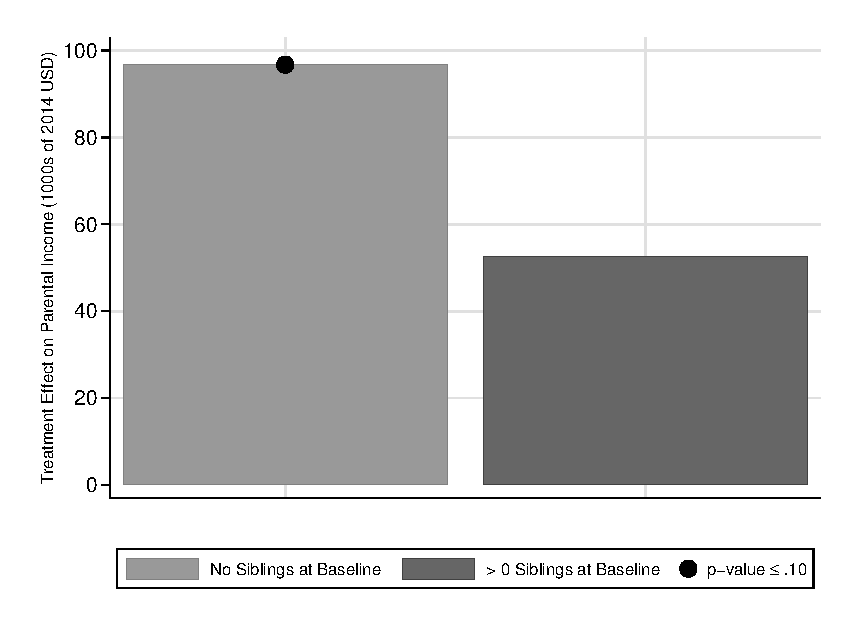
\includegraphics[width=\textwidth]{output/abccare_pincomesum_spooled.eps}
\end{subfigure}%
\begin{subfigure}[h]{0.5\textwidth}
		\centering
		\caption{Siblings Younger than 5 vs. Siblings 5 or Older}
		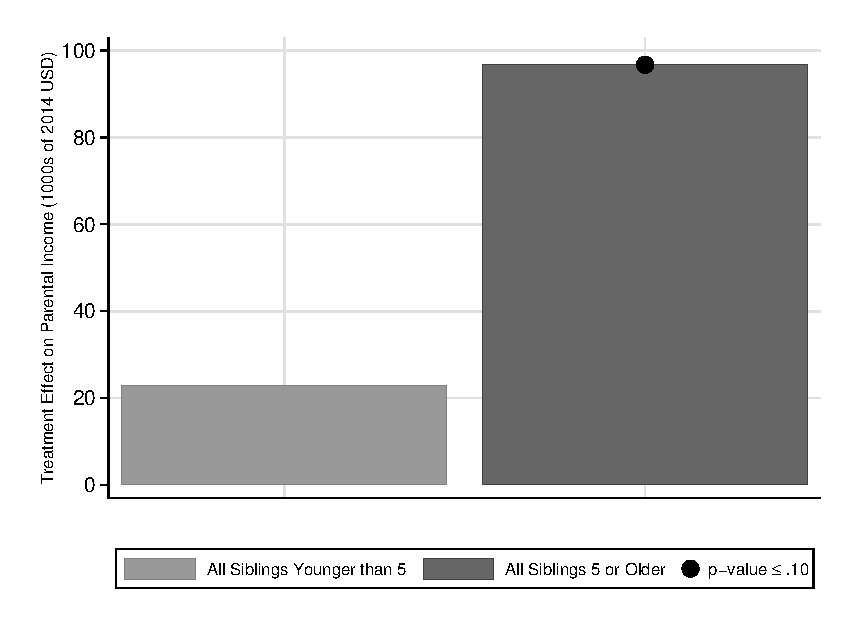
\includegraphics[width=\textwidth]{output/abccare_pincomesumsibage_spooled.eps}
\end{subfigure}
\footnotesize \justify
Note: Panel (a) displays the net-present value (treatment less control) of parental income of parents of children with and without siblings at baseline. Panel (b) displays the average parental income of parents of children with young siblings (younger than 5 years old) and children with older siblings (5 years old or older) at baseline. Panel (b) drops children without siblings at baseline. Parental income is in 2014 USD discounted to child's participant age 0 using a 3\% rate. We use the baseline ``conservative'' measure of parental income in Section~\ref{section:pincome}. Results using our alternative parental income measures are similar (see Appendix~\ref{app:parentalincome}).
\end{figure}

\paragraph{Using Mincer Equations to Predict Parental Income} \label{appendix:mincerpar}

\noindent This approach fits Mincer regressions for parental income.\footnote{See \citet{Mincer_1974_schooling} for the original source and \citet{Heckman_Lochner_ea_2006_HEE} for a extended discussion of the Mincer equation, its implications, and several extensions.} We specify how we deal with the presence of a spouse below. The parameterization used is as follows:

\begin{equation}
\ln Y_{a} = \alpha + \beta \cdot \text{school}_{a} + \gamma_{1}  \cdot \text{experience}_{a} + \gamma_{2} \cdot {\text{experience}_{a}}^2 + \bm{\psi} \mathbf{X}_{a} + \eta_{a}, \label{eq:mincer}
\end{equation}

\noindent where variables are indexed by mother's age, $\ln Y_a$ is log-labor income at age $a$, experience and schooling are measured in years, $ \mathbf{X}_{a}$ are observed characteristics, and $\eta_{a}$ is an unobserved component. $\alpha, \beta, \gamma_{1}, \gamma_{2}, \bm{\psi}$ are coefficients and summarize the parameterization of the labor income profile.\footnote{We assign one dollar of income when parental income is reported to be zero.}\\

\noindent In principle, there is no reason why the parameters characterizing the profile should differ across the treatment and control groups in ABC/CARE. Given the small sample in ABC/CARE, we assume that the profile is common across the control and treatment groups. This assumption is analogous to Assumption~\ref{ass:summary}, which we fail to reject in Appendix~\ref{app:invariance}.\\

\noindent We estimate the coefficients in \eqref{eq:mincer} using the sample of mothers in ABC/CARE. We pool the longitudinal information and estimate the coefficients using ordinary least squares. We use a standard Mincer measure of experience (age - education - 6). We assign one dollar to mothers with no labor income. For mothers living with a working partner, we allocate $1/2$ of total parental income as $Y_{a}$. To validate our estimates within ABC/CARE, we estimate the coefficients \eqref{eq:mincer} using a sub-sample of disadvantaged mothers in the PSID.\footnote{We define disadvantaged as follows: Black, not married, labor income, education (at age 5 of child's participant), age and number of children (at age 5 of child's participant) in the same ranges as the ABC/CARE mothers, labor income below percentile 75.} The coefficients characterizing \eqref{eq:mincer} in ABC/CARE and PSID for different combinations of control sets are in agreement. We display them in Table~\ref{table:mincerpsid}.\\

\begin{table}[H]
\begin{threeparttable}
\caption{Mincer Equation Estimates for Mothers in ABC/CARE and the PSID}
\label{table:mincerpsid}
\centering
\footnotesize
\begin{tabular}{lcccccc} \toprule 
           & PSID & ABC/CARE & PSID & ABC/CARE & PSID \\ \midrule
Education & 0.08*** & 0.06*** & 0.12*** & 0.10*** & 0.11*** & 0.09*** \\
 & (0.01) & (0.02) & (0.01) & (0.02) & (0.01) & (0.02) \\
 Experience &  &  & 0.04*** & 0.09*** & 0.04*** & 0.09*** \\
 &  &  & (0.00) & (0.01) & (0.00) & (0.01) \\
Experience &  &  & -0.00*** & -0.00*** & -0.00*** & -0.00*** \\
 &  &  & (0.00) & (0.00) & (0.00) & (0.00) \\
 Birth Year &  &  &  &  & -0.00*** & 0.01 \\
 &  &  &  &  & (0.00) & (0.01) \\
 Children &  &  &  &  & -0.08*** & -0.05 \\
 &  &  &  &  & (0.01) & (0.04) \\
Constant & 8.28*** & 8.89*** & 7.36*** & 7.82*** & 15.64*** & -12.35 \\
 & (0.06) & (0.19) & (0.08) & (0.19) & (1.55) & (16.60) \\ \\ \midrule
Observations & 15,506 & 705 & 15,506 & 705 & 15,506 & 664 \\
 & 0.01 & 0.02 & 0.04 & 0.22 & 0.05 & 0.20 \\ \bottomrule
\end{tabular}

\begin{tablenotes}
\footnotesize
\item Note: This table presents estimates of \eqref{eq:mincer} for ABC/CARE mothers and a subsample of disadvantaged mothers in the PSID. We define disadvantaged as follows: Black, not married, labor income, education (at age 5 of child's participant), age and number of children (at age 5 of child's participant) in the same ranges as the ABC/CARE mothers, labor income below percentile 75. Robust standard errors are in parentheses. $p$-value $< .01$. $^{**}$: $p$-value $< .05$. $^{*}$: $p$-value $< .10$.
\end{tablenotes}
\end{threeparttable}
\end{table}

\noindent Based on the estimates in Table~\ref{table:mincerpsid}, we can ask two questions: (i) what is the predicted net present value of parental income (treatment - control) using a prediction based on the estimate of \eqref{eq:mincer} and how does it differ from the method that linearly interpolates income from child's age 0 to 21?; and (ii) what would be the predicted net present value of parental income if we go beyond and predict all the way up to 40 years of experience?\\

\noindent Table~\ref{table:psens} display results that answer these two questions. Precise estimates for \eqref{eq:mincer} are obtained. From it we can measure (treatment - control) when the subjects are 21 years old. When using these same equations to predict parental labor income such that mothers work for 40 years in their life times, we find that we add $\$30,000$ (2014 USD) to the estimate reported in the main paper.

\begin{table}[H]
\begin{threeparttable}
\caption{Parental Labor Income, Interpolations and Prediction}
\label{table:psens}
\centering
\begin{tabular}{lccc} \toprule
 & Males and Females  & Male  & Female  \\  \midrule
 Interpolated up to Age 21 & 82,287 & 65,477 & 96,251 \\
 & (22,981.46) & (26,603.57) & (32,000.64) \\
Mincer-based up to Age 21 &  75,114 &  72,030 &  78,198 \\  
 & (428.340) & (647.017) & (557.716) \\  
Mincer-based up to Retirement &  106,957 &  102,556 &  111,338 \\  
 & (609.870) & (921.222) & (794.076) \\  
\bottomrule \end{tabular} 

\begin{tablenotes}
\footnotesize
\item Note:  Interpolated up to Age 21: linearly interpolated parental income from (child's) age 0 to 21. Mincer-based up to Age 21: prediction from (child's) age 0 to 21 based on estimates coefficients of \eqref{eq:mincer} (full control set). Mincer-based up to Retirement: prediction from (child's) age 0 to mother's retirement (40 years of labor force participation assumed) based on estimates coefficients of \eqref{eq:mincer} (full control set). All values are in 2014 USD discounted to child's age 0. Standard errors in parentheses are based on the empirical bootstrap distribution.
\end{tablenotes}
\end{threeparttable}
\end{table}

\paragraph{Life-cycle Prediction of Parental Income} \label{appendix:lcyclepincome}

\noindent The third approach is to predict parental income as in Section~\ref{section:cbamethodology}. For want of maternal characteristics enabling us to construct synthetic treatment and control groups, we skip the matching procedure and directly implement the prediction. That is, we do not construct a synthetic control and treatment groups to fit the dynamic relationships in the auxiliary samples. Instead, we assume that all parental income is earned by the mother and limit the sample to Black females whose labor income at each age is below the in-sample 90th percentile (we calculate this for the PSID and NLSY79 separately before using them jointly as one sample). As with labor income (of program participants) after age 30, we use the PSID and NLSY79 as one sample. For the same lack of data, we use a single predictor: lagged parental income. We initialize the prediction with the last observed measure of maternal income and extrapolate until the mother is 65 years old. Figure~\ref{figure:pincomeapp} displays our estimate of parental income in a format similar to Figure~\ref{figure:pincome}.\\

\begin{figure}[!htbp]
\centering
\caption{Discounted Net-present Value of Parental Income by Participant's Number and Age of Siblings at Baseline}\label{figure:pincomeapp}
\begin{subfigure}[h]{0.5\textwidth}
		\centering
		\caption{No Siblings vs. $>0$ Siblings}
		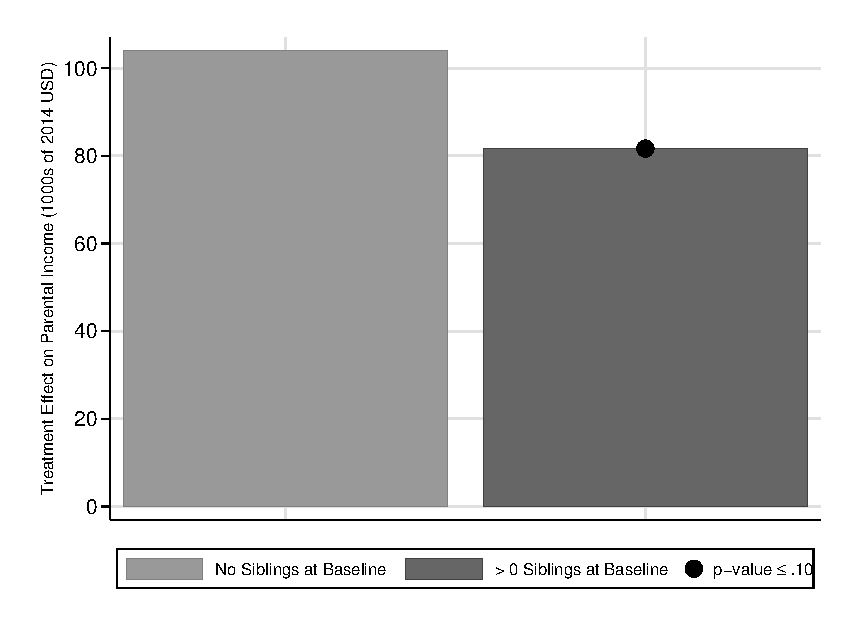
\includegraphics[width=\textwidth]{output/abccare_pinc_npv_pooled.eps}
\end{subfigure}%
\begin{subfigure}[h]{0.5\textwidth}
		\centering
		\caption{Siblings Younger than 5 vs. Siblings 5 or Older}
		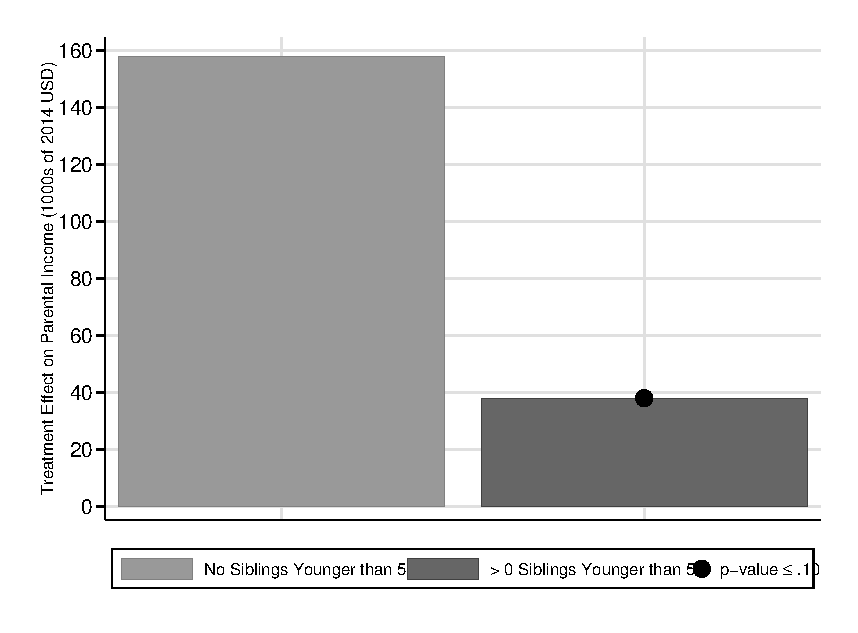
\includegraphics[width=\textwidth]{output/abccare_pinc_npv_sibs5_pooled.eps}
\end{subfigure}
\footnotesize \justify
Note: Panel (a) displays the net-present value (treatment less control) of parental income of parents of children with and without siblings at baseline. Panel (b) displays the average parental income of parents of children with young siblings (younger than 5 years old) and children with older siblings (5 years old or older) at baseline. Panel (b) drops children without siblings at baseline. Parental income is in 2014 USD discounted to child's participant age 0 using a 3\% rate.  We use the measure of parental income in Section~\ref{section:pincome}.
\end{figure}

\noindent \textbf{Summary: Prediction of Parental Labor Income}\\
\noindent Any prediction of parental income starts at the last observation of parental income, which varies by individual due to attrition. For prediction, we assume that parental income is equal to maternal income (only 27\% of mothers in ABC/CARE report leaving with a couple).
\begin{enumerate}
\item \textbf{Mincer Model}
\begin{enumerate}
\item \textbf{Auxiliary Sample Used to Predict:} PSID.
\item \textbf{Initial Restrictions Placed on the Auxiliary Sample:} Black; female; unmarried; education and number of children at ages 5 in the ranges of ABC/CARE participants, labor income at each age is below the 75th percentile.
\item \textbf{Variables Used to Construct Synthetic Control and Treatment Groups:} we pool PSID/NLSY79 restricted sample, and do not construct synthetic experimental groups due to lack of variables to do so.
\item \textbf{Variables Used to Predict:} education, second order polynomial in experience, birth year, number of children.
\item \textbf{Assumed Retirement:} after 40 years of labor force participation.
\end{enumerate}
\item \textbf{Life-cycle Prediction}
\begin{enumerate}
\item \textbf{Auxiliary Sample Used to Predict:} PSID and NLSY79.
\item \textbf{Initial Restrictions Placed on the Auxilliary Sample:} Black; female; labor income at each age is below the 90th percentile.
\item \textbf{Variables Used to Construct Synthetic Control and Treatment Groups:} we pool the PSID restricted sample, and do not construct synthetic experimental groups due to lack of variables to do so.
\item \textbf{Variables Used to Predict:} lagged labor income.
\item \textbf{Assumed Retirement:} 65 years old.
\end{enumerate}
\end{enumerate}

\subsection{Internal Rate of Return}
\label{app:method_irr}

\noindent To estimate the internal rate of return, we solve for $\rho$ in the following equation:
\begin{align}
\sum_{a=0}^A \frac{ \mathbb{E} (B_a - C_a)}{(1+\rho)^a} = 0,
\end{align}
where we let $A = 79$, define $B_a$ and $C_a$ to be the (discounted) total benefits and costs of the program at age $a$, and define $\mathbb{E}(.)$ to be the sample mean.\footnote{This is an abuse of notation given that $B_a$ and $C_a$ are not discounted in Appendix~\ref{app:method_irr}.} That is, we estimate the internal rate of return for the \textit{average subject} of ABC/CARE. \\

\noindent All outcomes of the parents and subjects affected by the program are treated as benefits. For this to make sense, we reverse the sign of the monetized effect of the program on specific outcomes. Costs of ABC/CARE consist only of the initial program costs from ages 0 to 5. Table \ref{table:bc_comp} provides a full list of the benefits and costs of ABC. \\

\noindent We take the sum of the treatment effects on each component of the benefits to be the total benefit, $B_a$, of the ABC/CARE program. This includes parental income, subject labor income, and QALYs (quality-adjusted life years). Treatment effects on costs borne by the subject or society have their signs reversed and are included as benefits. We do this for subject public-transfer income, education costs, crime costs, control substitution costs, and health costs. To account for deadweight loss, we impose a marginal welfare cost of 50\% by multiplying public costs by a factor of $0.5$ when they are a direct transfer from the government to the individuals\footnote{There is no clear consensus on the marginal welfare cost of tax revenue. However, most researchers estimate the welfare cost per tax dollar to be between \$0.30 and \$0.50. See \citet{Feldstein_1999_REStat}, \citet{Heckman_Smith_1998_evaluating}, and \citet{Browning_1987_AER}.} When the public costs are not a direct transfer from the government to the individuals, we multiply them by a factor of $1.5$.\\

\noindent The principle for multiplying the public costs is the following. We evaluate the social benefits of ABC/CARE and do not place a value on who receives the money. The only social cost from a direct transfer is the dead-weight loss that it generates: $50\%$ of its total value. We do not consider education and criminal costs to be a direct transfer. Thus, we multiply them by a factor of $1.5$: the value of their cost plus $50\%$ of the value of their cost (the dead-weight loss implied in raising the public revenue to fund them). Table \ref{table:bc_comp} lists the factor we use to multiply each cost to account for its implied dead-weight loss.\\

\noindent Having constructed our cash flow, $\mathbb{E} (B_a - C_a)$, solving for $\rho$ reduces to an algebraic exercise. The expected life-cycle profile of net benefits need to satisfy a ``single crossing property'' in order to obtain a unique solution for the internal rate of return.\footnote{See \citet{Arrow-Levhari_1969_EJ} for a formal discussion, although the discussion on multiplicity, sign, and real or complex nature of the roots of a polynomial traces back to Descarte's Rule.} The single crossing property holds when the benefits do not go from positive to negative across the life cycle. When the single crossing property is not satisfied, the internal rate of return is not a valid summary for the efficiency of an investment. To calculate the internal rate of return, we estimate the treatment effect on each component of the benefits and costs at age $a$ for the pooled, male, and female samples. We do this for 100 bootstrap resamples of the original ABC/CARE data. In the case of health costs and subject income, for which we employ auxiliary datasets to estimate the treatment effects, we also obtain 100 bootstrap estimates from the auxiliary data for every ABC/CARE bootstrap resample, resulting in a total of 100,000 estimates. By reusing each bootstrap estimate of the treatment effect on outcomes that do not require any auxiliary data set 100 times, we obtain a total of 100,000 estimates of the cash flow. We estimate the internal rate of return on each of those cash flows, and discard those for which we find a negative internal rate of return. The remaining estimates form our empirical bootstrap distribution of the internal rate of return for the pooled, male, and female samples. We take the mean of the distributions to be the point estimates, and we take the sample standard deviations to be the standard errors. To construct the 80\% confidence intervals, we take the 10\textsuperscript{th} and 90\textsuperscript{th} quantiles of each bootstrap distribution.\\

\noindent Figure~\ref{figure:irrdist} reports the distributions of the internal rates of return, by gender and for each of the three parameters that we consider (treatment vs. next best, treatment staying at home, treatment vs. alternative preschool). For some parameters and genders, we discard a high percentage of the internal rate of return of the outcomes. We next discuss how we calculate the benefit/cost ratios, noting that this statistics is not subject the same caveat as the internal rate of return: we can summarize the efficiency of the investment even in the absence of the single-crossing property.

\newgeometry{top=.6in, bottom=.8in, left=.6in, right=.6in}
\begin{sidewaysfigure}[!htbp]
\centering
\caption{Internal Rate of Return, by Gender and by Parameter}\label{figure:irrdist}
\begin{subfigure}[h]{0.25\textwidth}
		\centering
		\caption{Treatment vs. Next Best, Pooled}
		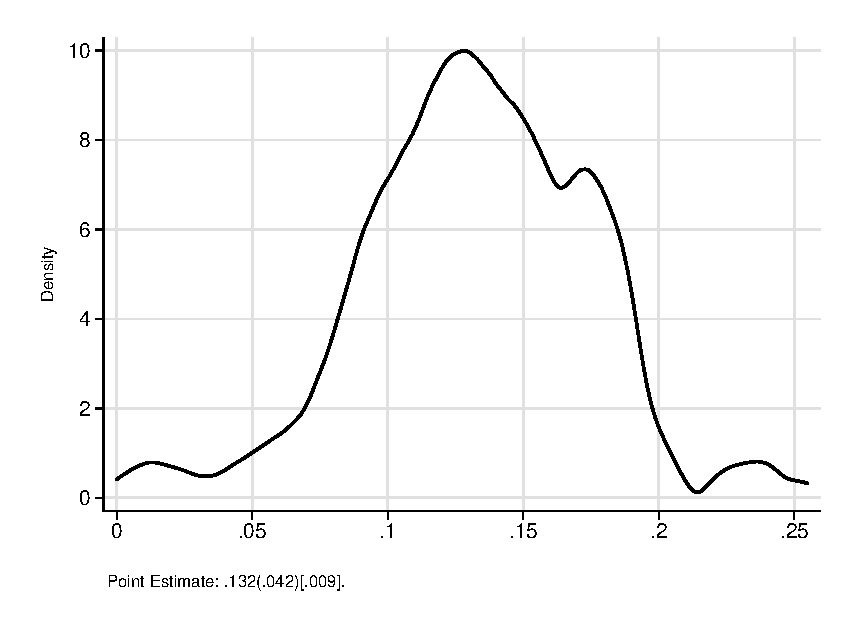
\includegraphics[width=\textwidth]{output/irr_2_sexp.eps}
\end{subfigure}%
\begin{subfigure}[h]{0.25\textwidth}
	\centering
	\caption{Treatment vs. Next Best,\\ Females}
		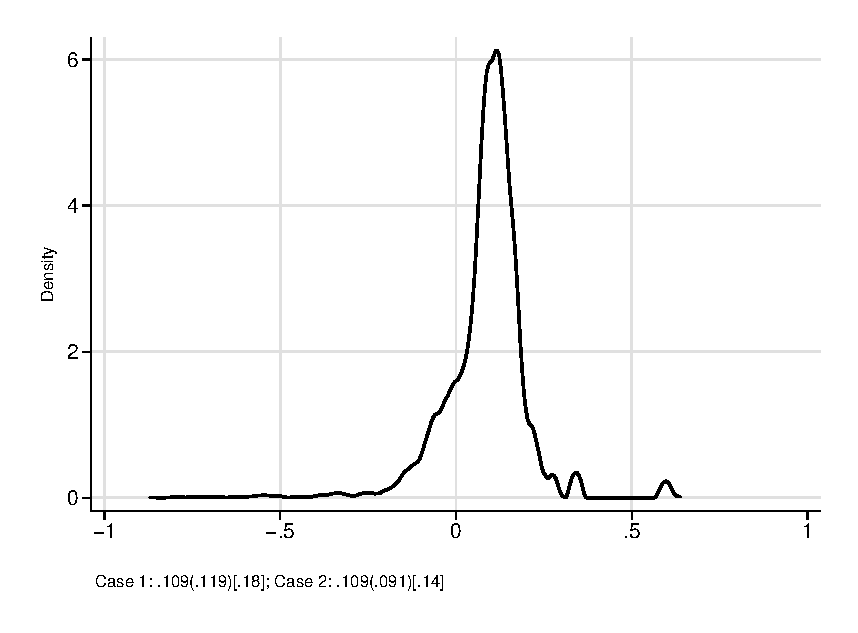
\includegraphics[width=\textwidth]{output/irr_2_sexf.eps}
\end{subfigure}%
\begin{subfigure}[h]{0.25\textwidth}
		\centering
		\caption{Treatment vs. Next Best, Males}
		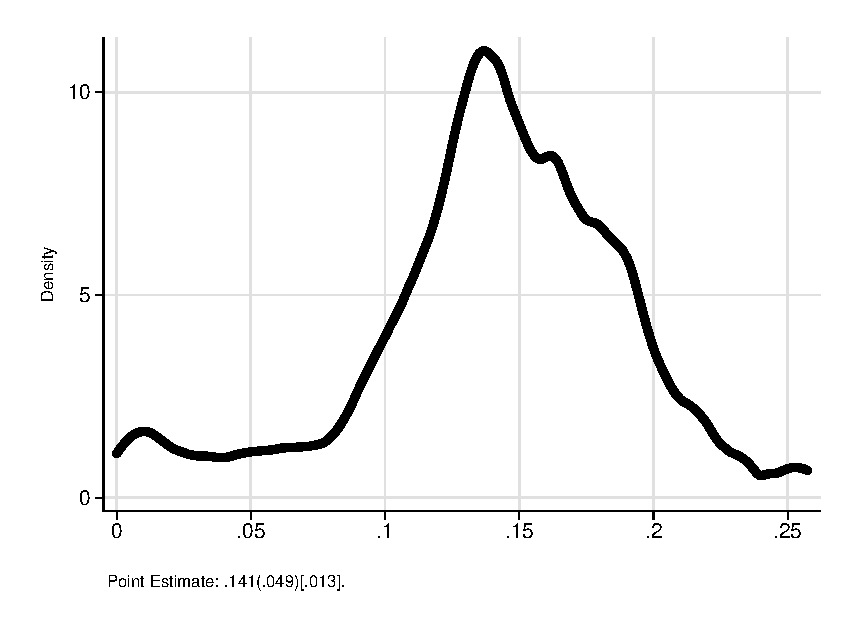
\includegraphics[width=\textwidth]{output/irr_2_sexm.eps}
\end{subfigure}
\begin{subfigure}[h]{0.25\textwidth}
	\centering
	\caption{Treatment vs. Staying at Home, Pooled}
		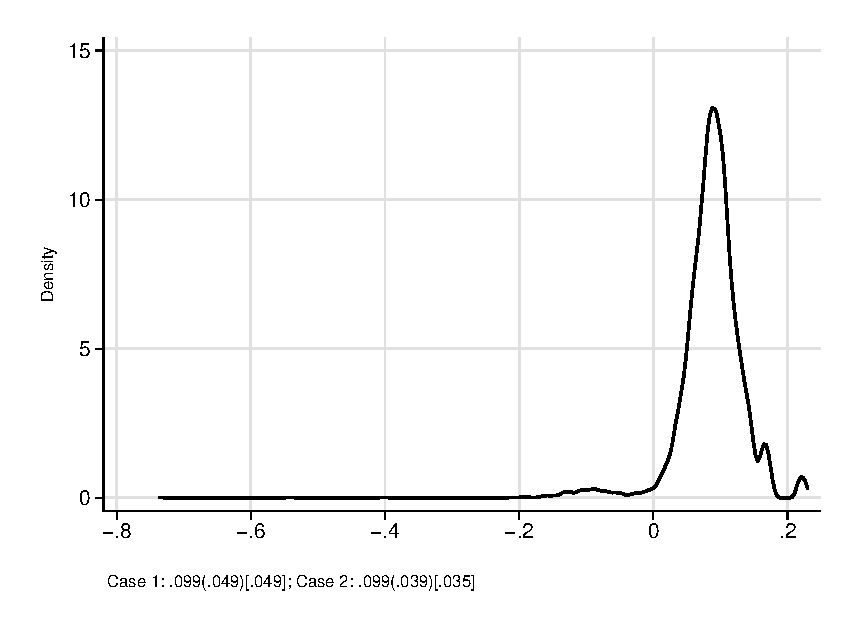
\includegraphics[width=\textwidth]{output/irr_5_sexp.eps}
\end{subfigure}%
\begin{subfigure}[h]{0.25\textwidth}
	\centering
	\caption{Treatment vs. Staying at Home, Females}
		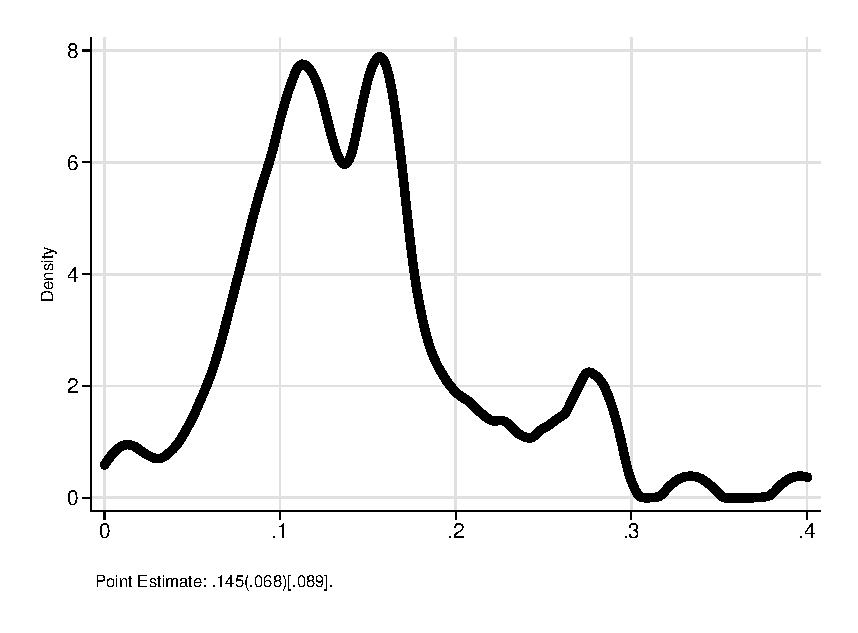
\includegraphics[width=\textwidth]{output/irr_5_sexf.eps}
\end{subfigure}%
\begin{subfigure}[h]{0.25\textwidth}
	\centering
	\caption{Treatment vs. Staying at Home, Males}
		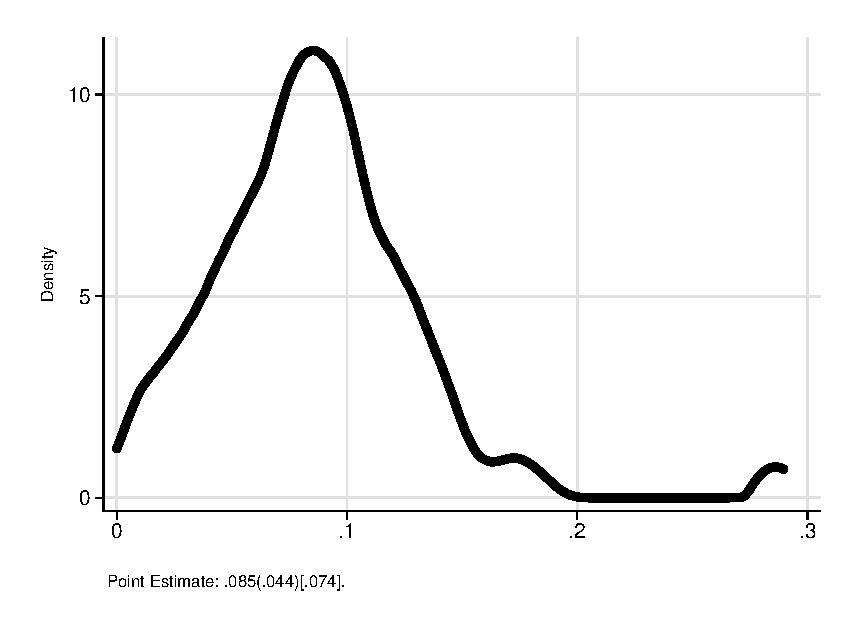
\includegraphics[width=\textwidth]{output/irr_5_sexm.eps}
\end{subfigure}
\begin{subfigure}[h]{0.25\textwidth}
	\centering
	\caption{Treatment vs. Alternative Preschool, Pooled}
		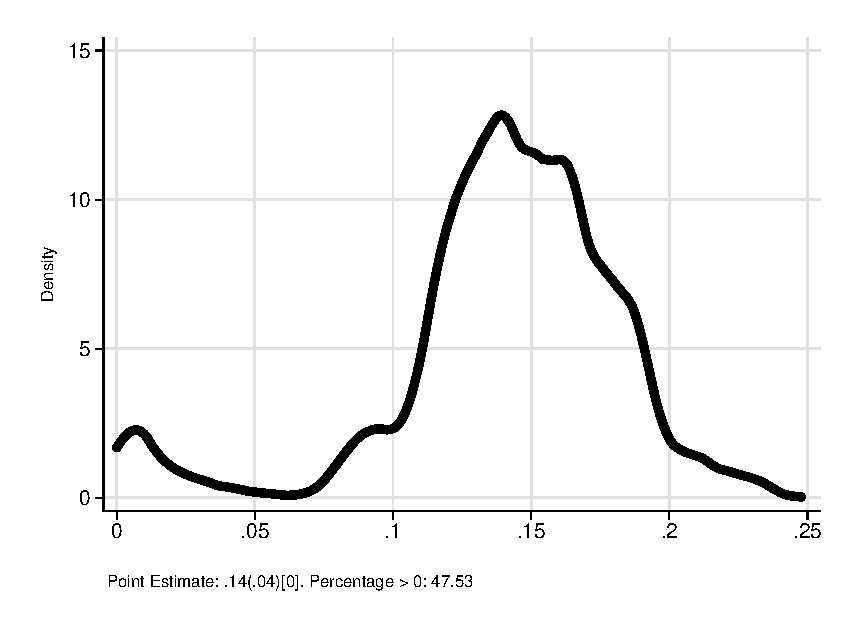
\includegraphics[width=\textwidth]{output/irr_8_sexp.eps}
\end{subfigure}%
\begin{subfigure}[h]{0.25\textwidth}
	\centering
	\caption{Treatment vs. Alternative Preschool, Females}
		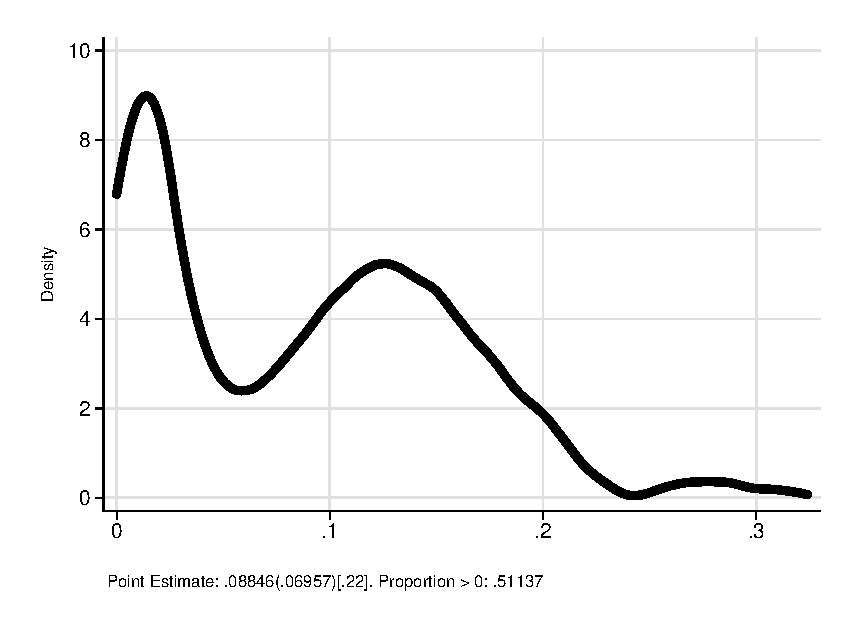
\includegraphics[width=\textwidth]{output/irr_8_sexf.eps}
\end{subfigure}%
\begin{subfigure}[h]{0.25\textwidth}
	\centering
	\caption{Treatment vs. Alternative Preschool, Males}
		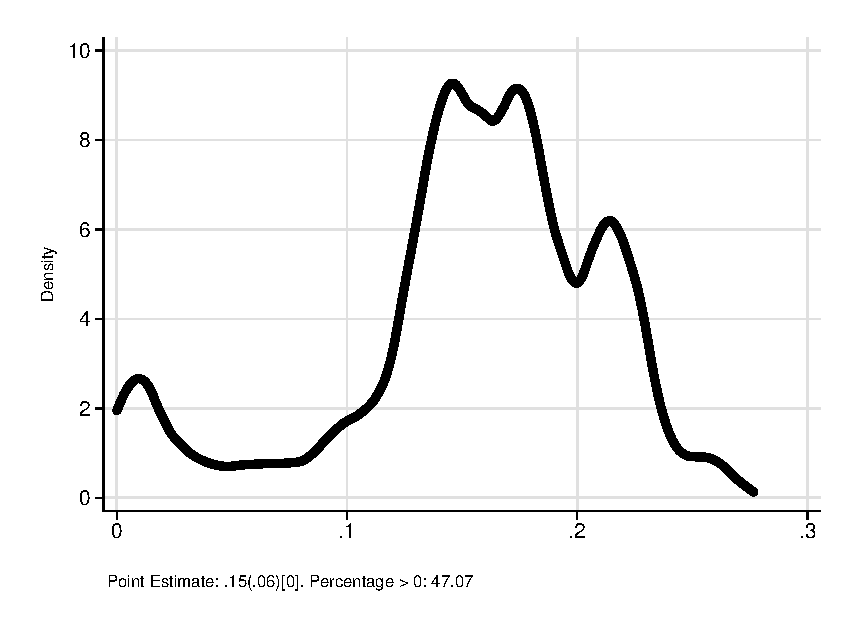
\includegraphics[width=\textwidth]{output/irr_8_sexm.eps}
\end{subfigure}
\footnotesize \justify
Note: Panel (a) displays the empirical bootstrap distribution for the estimate of the treatment vs. next parameter in the pooled sample. The reminder panels show an analogous distribution varying the parameter and the gender. See Section~\ref{section:methodsquestions} for the definition of the parameters. We discard negative internal rates of returns. Each panel displays the point estimate with the standard error in parentheses and the $p$-value in brackets in the left corner and the percentage of positive internal rates of return out of the initial set of bootstrap resamples in the right corner.
\end{sidewaysfigure}
\restoregeometry
\doublespacing



% We let $T = 79$. In Appendix \ref{app:method_identify}
% we explain how we can estimate the summand of the numerator at every period $t$, which
% can be expressed as $\mathbf{E}(B_t) -  \mathbf{E}(C_t)$. Thus, solving for $\rho$
% reduces to an algebraic exercise.



% To construct our cash flow, we subtract the costs from benefits to create a single stream.
% We define `cost' to include only the program costs of ABC, and define
% `benefits' to include all treatment effects of the program. This includes
% the treatment effects on parent income, subject labor income, and QALY
% (quality adjusted life years).\footnote{QALYs are measured on a scale of 0 to 1, with 1 being a
% year of perfect health. We follow \textbf{[CITATION]} and value a QALY of 1 to be
% \$150,000, and a QALY of 0 to be \$0. The dollar value of that year relates linearly to the QALY.}
% Treatment effects on costs borne by the subject or society have their signs
% reversed and are included as benefits. We do this for subject transfer income,
% education costs, jail costs, justice system costs, victimization costs,
% control contamination costs, and medical costs. To account for deadweight loss, we
% impose a marginal welfare cost of 50\% by multiplying public costs by a factor of
% $1.5$.\footnote{There is no clear consensus on the marginal welfare cost of tax revenue. However,
% most researchers estimate the welfare cost per tax dollar is between \$0.30--0.50. See
% \citet{feldstein1999tax, heckman1998evaluating, browning1987marginal}.} This
% includes education cost up until age 17, jail costs, justice system costs, Medicare costs,
% and Medicaid costs. For the same reason, we multiply transfer income by a factor of 0.5.

% For each period $t \in \{1, 2, \dots, 79\}$, we sum our estimates of the benefits, and
% subtract our estimates of the costs from that sum. This provides us an estimate of
% $\mathbf{E}(B_t) -  \mathbf{E}(C_t) = \mathbf{E} (B_t - C_t)$. We then solve for
% $\rho$ using numerical analysis.

% In your methodlogy you describe costs and benefits differnetly....
% To construct our cash flow, we sum the costs and benefits from the program into a single stream.
% We define `cost' to include only the cost of implementing ABC. On the other hand,
% we broadly define `benefits' to include all treatment effects of the program. This includes
% the treatment effects on parent income, subject labor income, and QALY
% (quality adjusted life years).\footnote{QALYs are measured on a scale of 0 to 1, with 1 being a
% year of perfect health. We follow \textbf{[CITATION]} and value a QALY of 1 to be
% \$150,000, and a QALY of 0 to be \$0. The dollar value of that year relates linearly to the QALY.}
% Treatment effects on outcomes generally considered to be costs have their signs reversed in
% order to convert them into benefits. We do this for subject transfer income,
% education costs, jail costs, justice system costs, victimization costs,
% control contamination costs, and medical costs. To account for deadweight loss, we
% impose a marginal welfare cost of 50\% by multiplying public costs by a factor of
% $1.5$.\footnote{There is no clear consensus on the marginal welfare cost of tax revenue. However,
% most researchers estimate the welfare cost per tax dollar is between \$0.30--0.50. See
% \citet{feldstein1999tax, heckman1998evaluating, browning1987marginal}.} This
% includes education cost up until age 17, jail costs, justice system costs, Medicare costs,
% and Medicaid costs. For the same reason, we multiply transfer income by a factor of 0.5.


\subsection{Computing the Benefit/Cost Ratio}\label{app:method_cbratio}

\noindent The benefit/cost ratio is
\begin{align}
\mathbb{E} \left( \frac{ \sum_{a=0}^A B_a}{\sum_{a=0}^A C_a} \right),
\end{align}

\noindent where we let $A = 79$, define $B_a$ and $C_a$ to be the benefits and costs of the
program at age $a$, and define $\mathbb{E}(.)$ to be the sample mean. See Table \ref{table:bc_comp} for a detailed list of the components
to the benefits and costs of ABC/CARE . We take the sum of the treatment effects on each component
of the benefits to be the total benefits of the ABC/CARE programs. \\

\noindent To account for deadweight loss, we assume a marginal welfare cost of 50\% by multiplying
public costs components by a factor of $1.5$. For the same reason, we multiply public-transfer
income by a factor of 0.5. We discount each component of the benefits and costs
by 3\% every year to obtain their net present value at birth. We then sum up the discounted
components of the benefits and find the ratio with the discounted costs. \\

\noindent We estimate the treatment effect for each component of the benefits and costs at age $a$ for the pooled, male, and female samples. We do this for 100 bootstrap resamples of the original ABC/CARE data. In the case of health and subject income, for which we employ auxiliary datasets to estimate the treatment effects, we also obtain 100 bootstrap estimates from the auxiliary data for every ABC/CARE bootstrap resample, resulting in a total of 100,000 estimates. By reusing each bootstrap estimate of the treatment effect on outcomes that do not require any auxiliary data set 100 times, we obtain a total of 100,000 estimates of the costs stream and benefits stream. We estimate the benefit/cost ratio for each of those streams. This is how we form our empirical bootstrap distribution of the benefit/cost ratio for the pooled, male, and female samples. We take the mean of the distributions to be the point estimates, and we take the standard deviations to be the standard errors. To construct the 80\% confidence intervals, we take the 10\textsuperscript{th} and 90\textsuperscript{th} quantiles of each bootstrap distribution. Figure~\ref{figure:ratiodist} presents the empirical distribution of the empirical bootstrap distribution, per parameter of interest and gender.

\begin{table}[H]
\begin{threeparttable}
\caption{Components of Benefits and Costs}
\label{table:bc_comp}
\centering
\begin{tabular}{l c c}
\toprule			
Variable & Sign Reversed	& Welfare Cost \\
	&		& Factor \\
\midrule
\textbf{Benefits} 	\\			
\quad Parent Income			& \\
\quad Subject QALY			& \\
\quad Subject Labor Income	& \\
\quad Subject Public-transfer Income	& $\checkmark$	& 0.5 \\
\quad Medicare Costs			& $\checkmark$	& 1.5 \\
\quad Medicaid Costs			& $\checkmark$	& 1.5 \\
\quad Out-of-pocket Medical Costs	& $\checkmark$ \\
\quad Miscellaneous Medical Costs	& $\checkmark$ \\
\quad Disability Insurance Claim	& $\checkmark$	&	1.5 \\
\quad Social Security Claim	& $\checkmark$	&	1.5 \\
\quad Supplemental Security Claim	& $\checkmark$	&	1.5 \\
\quad Control Substitution Costs	& $\checkmark$	& \\
\quad Education Costs			& $\checkmark$	& 1.5* \\
\quad Justice System Costs	& $\checkmark$	& 1.5 \\
\quad Prison Costs			& $\checkmark$	& 1.5 \\
\quad Victimization Costs		& $\checkmark$	& \\
\textbf{Costs} 	\\			
\quad Program Costs			& \\
\bottomrule			
\end{tabular}
\begin{tablenotes}
\footnotesize
\item Note: The table lists the components of the costs and benefits of ABC/CARE.
In order for some components to be categorized as benefits, we reversed the sign
of the treatment effect. *Only education costs up until age 18 are multiplied by 1.5 to account for welfare costs. This factor is drawn from \citet{Heckman_Moon_etal_2010_RateofReturn}.
\end{tablenotes}
\end{threeparttable}
\end{table}

\newgeometry{top=.6in, bottom=.8in, left=.6in, right=.6in}
\begin{sidewaysfigure}[!htbp]
\centering
\caption{Benefit/Cost Ratios, by Gender and by Parameter}\label{figure:ratiodist}
\begin{subfigure}[h]{0.25\textwidth}
		\centering
		\caption{Treatment vs. Next Best, Pooled}
		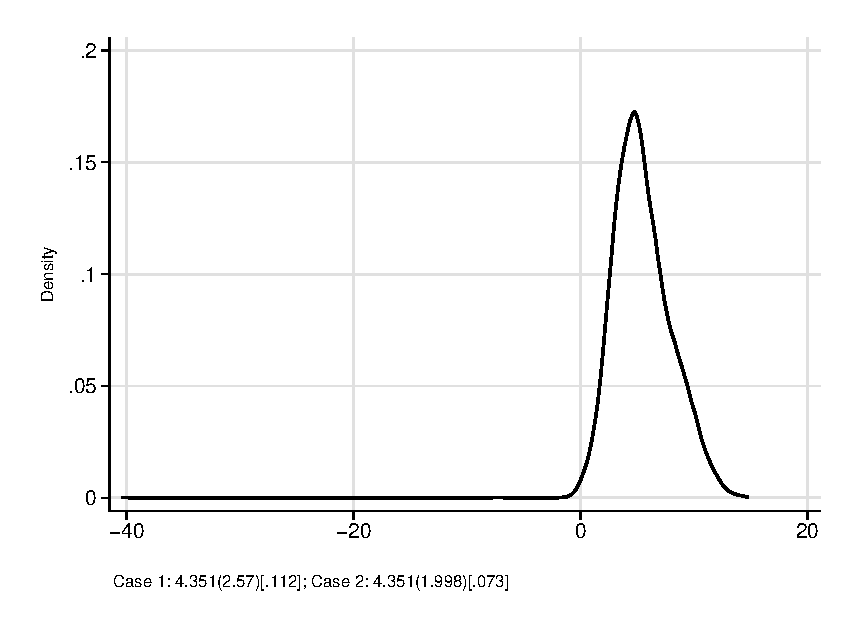
\includegraphics[width=\textwidth]{output/ratios_2_sexp.eps}
\end{subfigure}%
\begin{subfigure}[h]{0.25\textwidth}
	\centering
	\caption{Treatment vs. Next Best,\\ Females}
		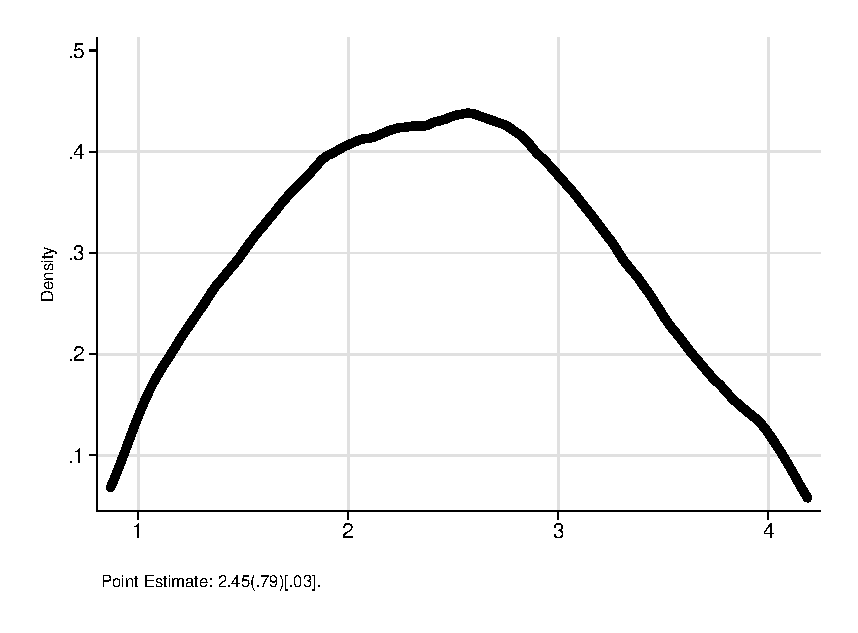
\includegraphics[width=\textwidth]{output/ratios_2_sexf.eps}
\end{subfigure}%
\begin{subfigure}[h]{0.25\textwidth}
		\centering
		\caption{Treatment vs. Next Best, Males}
		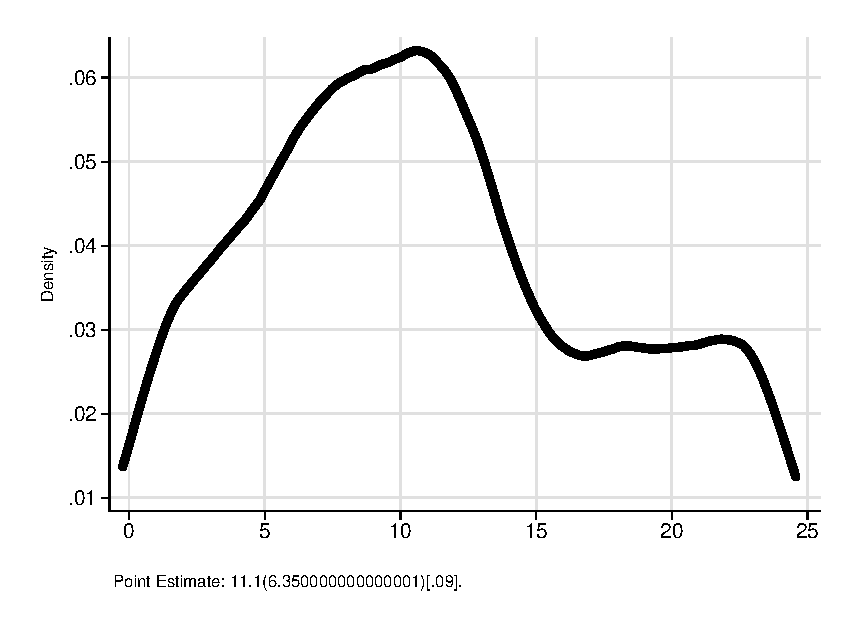
\includegraphics[width=\textwidth]{output/ratios_2_sexm.eps}
\end{subfigure}
\begin{subfigure}[h]{0.25\textwidth}
	\centering
	\caption{Treatment vs. Staying at Home, Pooled}
		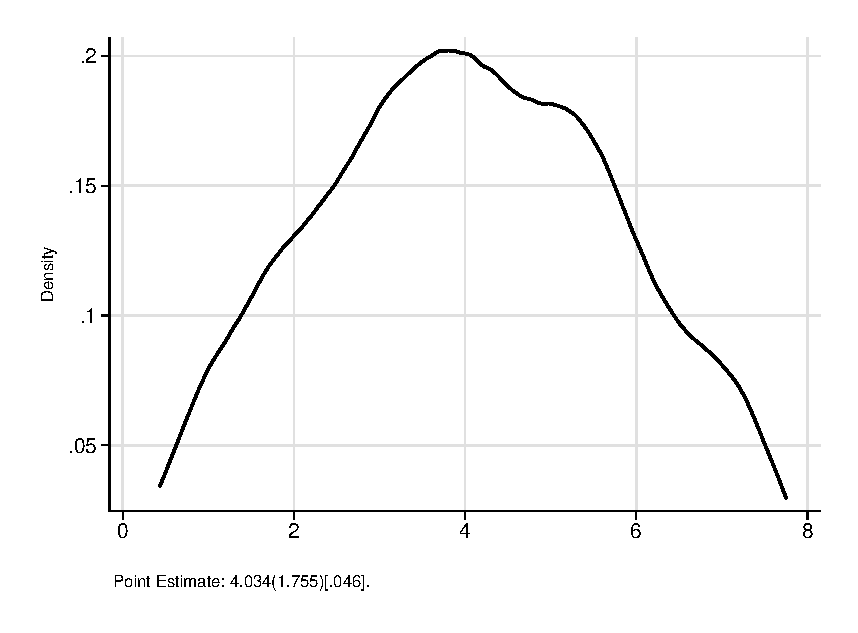
\includegraphics[width=\textwidth]{output/ratios_5_sexp.eps}
\end{subfigure}%
\begin{subfigure}[h]{0.25\textwidth}
	\centering
	\caption{Treatment vs. Staying at Home, Females}
		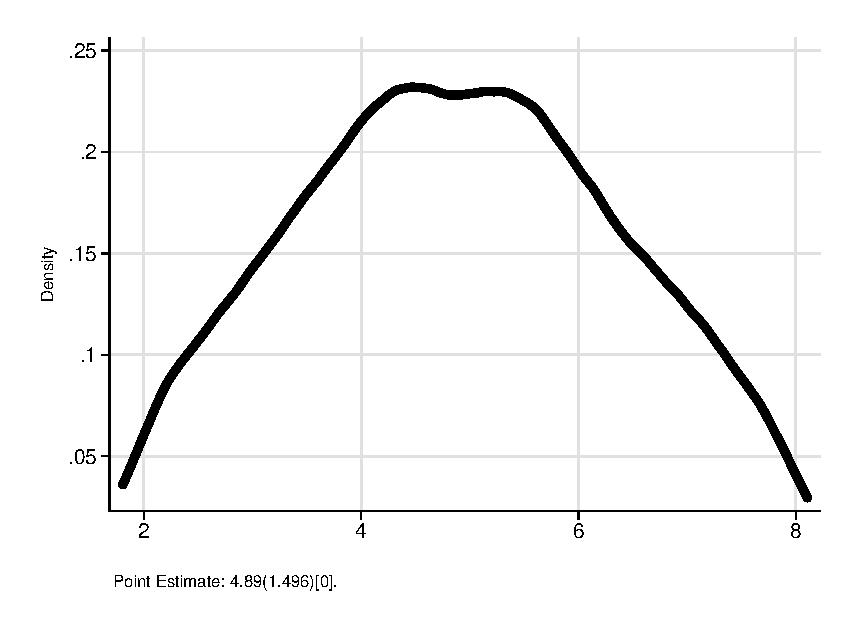
\includegraphics[width=\textwidth]{output/ratios_5_sexf.eps}
\end{subfigure}%
\begin{subfigure}[h]{0.25\textwidth}
	\centering
	\caption{Treatment vs. Staying at Home, Males}
		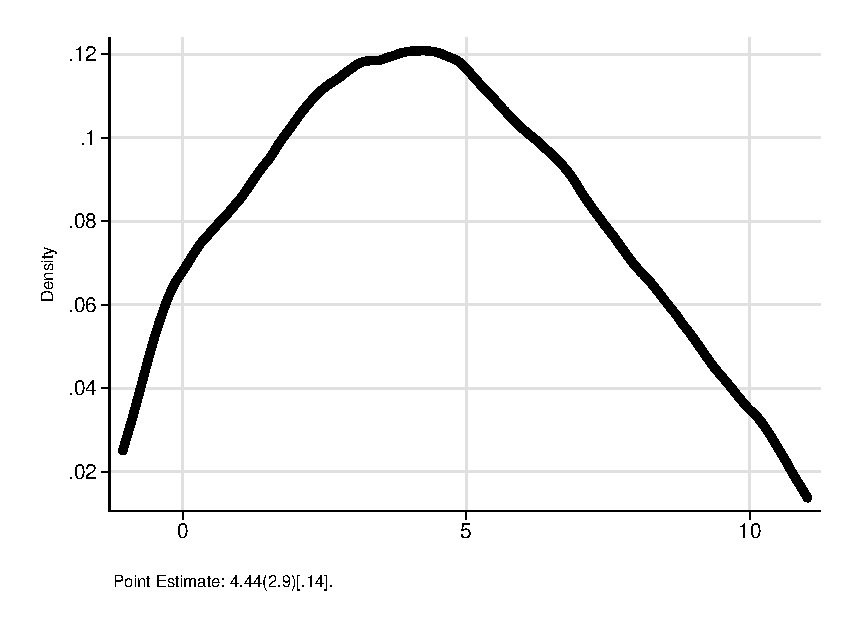
\includegraphics[width=\textwidth]{output/ratios_5_sexm.eps}
\end{subfigure}
\begin{subfigure}[h]{0.25\textwidth}
	\centering
	\caption{Treatment vs. Alternative Preschool, Pooled}
		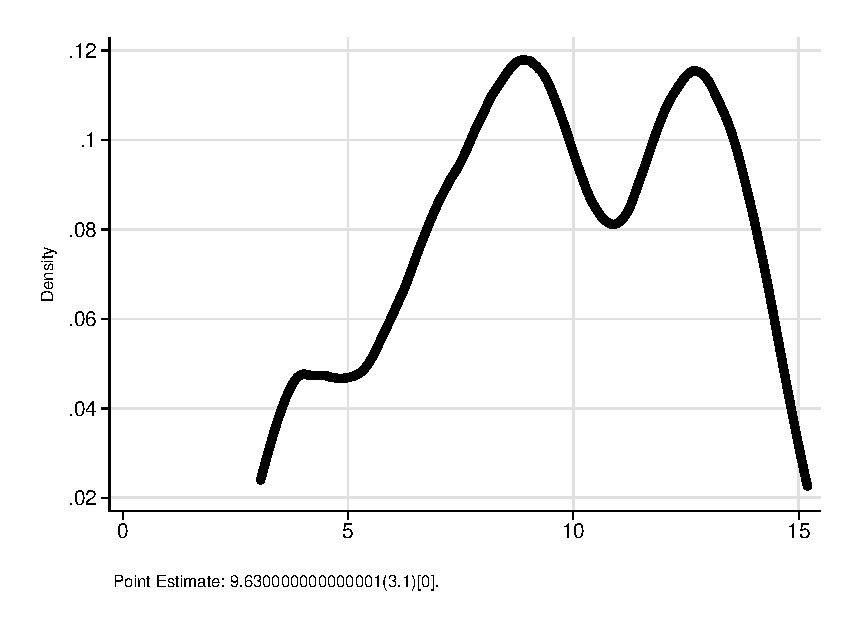
\includegraphics[width=\textwidth]{output/ratios_8_sexp.eps}
\end{subfigure}%
\begin{subfigure}[h]{0.25\textwidth}
	\centering
	\caption{Treatment vs. Alternative Preschool, Females}
		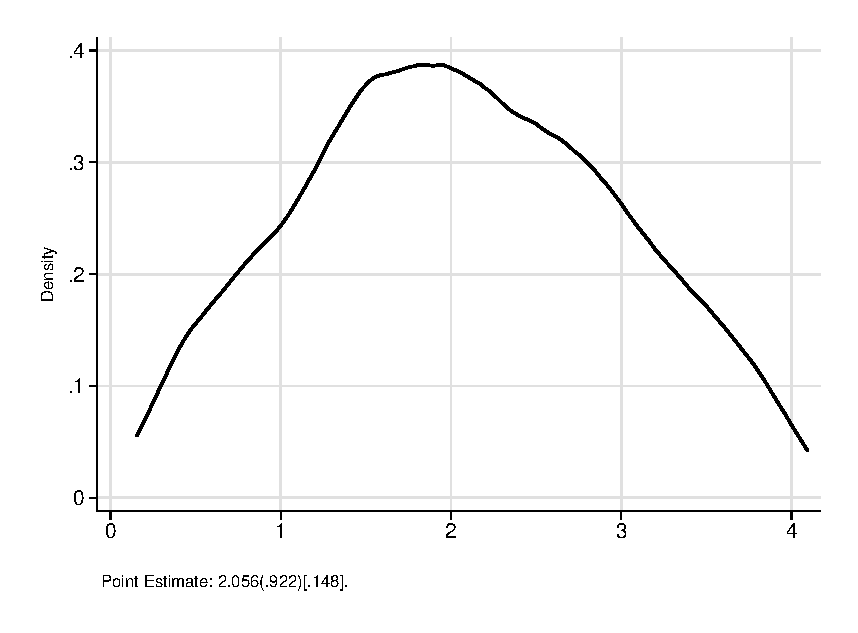
\includegraphics[width=\textwidth]{output/ratios_8_sexf.eps}
\end{subfigure}%
\begin{subfigure}[h]{0.25\textwidth}
	\centering
	\caption{Treatment vs. Alternative Preschool, Males}
		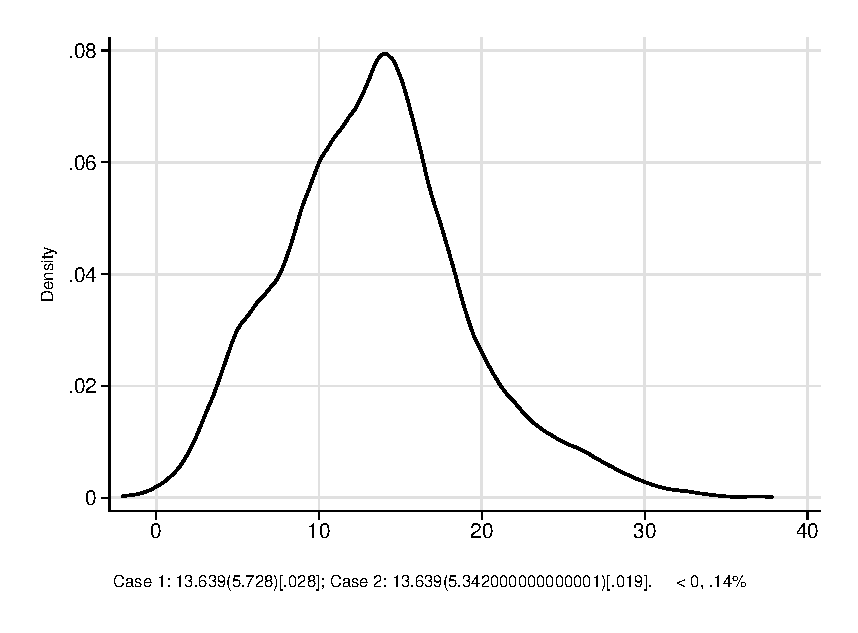
\includegraphics[width=\textwidth]{output/ratios_8_sexm.eps}
\end{subfigure}
\footnotesize \justify
Note: Panel (a) displays the empirical bootstrap distribution for the estimate of the treatment vs. next parameter in the pooled sample. The reminder panels show an analogous distribution varying the parameter and the gender. See Section~\ref{section:methodsquestions} for the definition of the parameters. Each panel displays the point estimate with the standard error in parentheses and the $p$-value in brackets in the left corner.
\end{sidewaysfigure}
\restoregeometry
\doublespacing

\subsection{Exploring the Impact of Using Different Prediction Models} \label{appendix:predsensitivity}
\noindent \textbf{[JLG: All your requests to this section have been completed.]}\\

\noindent Our analysis is based on a causal model for treatment ($d=1$) and control ($d=0$) outcomes for measure $j$ at age $a$ in sample $k \in \{e,n\}$ where $e$ denotes membership in the experimental sample and $n$ denotes membership in the auxiliary sample:

\begin{equation}\label{eq:outcome}
Y^d_{k,j,a} = \phi^d_{k,j,a} (\bm{X}^d_{k,a}, \bm{B}_k) + \varepsilon^d_{k,j,a}, \quad k \in \{n,e\}, \quad j \in \mathcal{J}_a, \quad d \in \{0, 1\}.
\end{equation}

\noindent $\phi^d_{k,j,a}\left( \cdot, \cdot \right)$ is an invariant structural production relationship mapping inputs $\bm{X}^d_{k,a}, \bm{B}_k$ into output $Y^d_{k,j,a}$ holding error term $\varepsilon^d_{k,j,a}$ fixed.\\ 

\noindent In this appendix, we layout different structures for $\phi_{k,j,a}^d \left( \cdot, \cdot \right)$ and $\varepsilon_{k,j,a}^d$ and investigate the robustness of our estimates to different assumptions about the structure of both these elements. We do this exercise for labor income. In Appendix~\ref{appendix:gmm}, we describe the precise steps that we follow to construct out-of-sample predictions based on these different structures and frame our estimations in a general method of moments framework.\\ 

\begin{equation}
\varepsilon^d_{k,j,a} = \rho \varepsilon^d_{k,j,{a-1}} + \eta_{k,j,{a}} \label{eq:error}
\end{equation}

\noindent where $\eta_{k,j,{a}}$ is i.i.d. and satisfies Assumption ~\ref{ass:exog} (Exogeneity).\\

\noindent It is also possible to extend the process in Equation~\eqref{eq:error} to account for an individual fixed effect. We explore this possibility below.\\ 

\noindent Table~\ref{table:predsens} summarizes the results from this exploration through two statistics: (i) the net present value (discounted to birth treatment - control) of predicted labor income under different assumptions; and (ii) the overall cost-benefit ratio when the predictions are done based on the different proposed alternatives. The results indicate that the model that we base our predictions on in the main text has little sensitivity to the deviations that we propose.

\begin{table}[H] 
\begin{threeparttable}
\caption{Net Present Value of Labor Income and Cost/Benefit Analysis Under Different Specifications for Labor Income Predictions}
\label{table:predsens}
\centering 
\footnotesize
\begin{tabular}{L{2cm} *7{C{1.5cm}}} \toprule
& \multicolumn{3}{c}{ \textbf{Specification 1:}} & & \multicolumn{3}{c}{ \textbf{Specification 2:}}\\
& \multicolumn{3}{c}{Lagged component in $\bm{\phi}_{j,a}$} & & \multicolumn{3}{c}{No lagged component in $\bm{\phi}_{j,a}$} \\
& \multicolumn{3}{c}{ set $\bm{\rho} = 0$} & & \multicolumn{3}{c}{Unrestricted $\bm{\rho}$} \\[10pt]
 
& NPV & IRR & B/C & & NPV & IRR & B/C \\
 
\hline \\
Pooled & 71,345 & 0.13 & 6.29 & & 154,547 & 0.26 & 12.39 \\ 
& (86,343) & (.05) & (2.11) & & (187,036) & (0.11) & (5.16) \\ \\
 
Males & 300,896 & 0.13 & 11.1 & & 200,509 & 0.09 & 7.62 \\ 
& (241,588) & (0.06) & (6.35) & & (160,988) & (0.04) & (3.73) \\ \\
 
Females & 59,390 & 0.10 & 2.45 & & 79,441 & 0.15 & 3.61 \\ 
& (63,060) & (0.07) & (0.79) & & (99,416) & (0.11) & (1.56) \\ \\ \\
 
\midrule
& \multicolumn{3}{c}{ \textbf{Specification 3:}} & & \multicolumn{3}{c}{ \textbf{Specification 4:}}\\
& \multicolumn{3}{c}{Lagged component in $\bm{\phi}_{j,a}$} & & \multicolumn{3}{c}{Lagged component in $\bm{\phi}_{j,a}$; Permanent} \\
& \multicolumn{3}{c}{Unrestricted $\bm{\rho}$} & & \multicolumn{3}{c}{Transitory unobserved components} \\[10pt]
 
& NPV & IRR & B/C & & NPV & IRR & B/C \\
 
\hline \\
Pooled & 268,179 & 0.49 & 23.64 & & 144,012 & 0.26 & 12.7 \\
& (211,089) & (0.12) & (5.16) & & (70,566) & (0.04) & (1.72) \\ \\
 
Males &456,078 & 0.2 & 16.82 & &240,921 & 0.1 & 8.89 \\ 
& (358,534) & (0.09) & (9.42) & &(124,129) & (0.03) & (3.26) \\ \\
 
Females & 31,303 & 0.05 & 1.29 & &34,590 & 0.06 & 1.43 \\ 
& (168,160) & (0.19) & (2.11) & &(53,611) & (0.06) & (0.67) \\ \\ \\
 
 
\midrule
& & & \multicolumn{3}{c}{\textbf{Specification 5:}} \\
& & & \multicolumn{3}{c}{ Fully Non-Parametric} \\[10pt]
& & & NPV & IRR & B/C \\
\hline \\
& & Pooled & 62,080 & 0.10 & 4.98 \\ 
& & & (75,030) & (0.03) & (2.07) \\ \\ 
& & Males & 289,471 & 0.13 & 11.01 \\ 
& & & (232,471) & (0.06) & (5.39) \\ \\ 
& & Females & 59,163 & 0.11 & 2.69 \\ 
& & & (74,039) & (0.08) & (1.16) \\ \bottomrule
\end{tabular}
\begin{tablenotes}
\footnotesize
\item Note: This table displays the net present value of labor income in 2014 USD (treatment - control) using the four different specifications for prediction that are explained below. Specification 1 is what we present in the main text. It also presents the calculation of the internal rate of return and the benefit-cost ratio of the program using these different net present values.
\end{tablenotes}
\end{threeparttable}
\end{table}

\noindent In the auxiliary sample, we observe the outcome $Y_{n,j,a}$ for $a \in [a^*, \ldots, A]$. In the experimental sample, we observe the outcome $Y_{e,j,a}$ for at most two ages, depending on the outcome. For the time being, suppose that we observe the outcome at one age ($a = a^*$). We come back to this below. By out-of-sample predictions we mean using the information in the auxiliary sample at  $a \in [a^*, \ldots, A]$ to form extrapolations in the experimental sample, where we do not observe the outcome of interest during this age periods. We produce out-of-sample predictions and calculate the net present value of labor income (treatment - control) under different structures.\\ 

\subsubsection{Specification 1: Lagged Component in $\phi_{j,a}$ and No Serial Correlation} \label{app:spec1}

\noindent In this specification, we assume that (i)  $Y_{k,j,a-1}$ is one of the elements in $\bm{X}_{k,a}$; and (ii) $\rho = 0$ in Equation~\eqref{eq:error}, and therefore Assumption ~\ref{ass:exog} (Exogeneity) holds for $\varepsilon_{k,j,a}^d$.\\

\noindent \textbf{We note the following on this specification:}

\begin{enumerate}
 
\item The predictions across the paper are constructed under this framework: labor and transfer income, crime, and health. 
\item Our comparison between realizations and predictions work quite well, as displayed in Figure~\ref{fig:labor-income-profiles} of the main text. 
\item Additional tests show the following. We fail to reject: invariance across the treatment and the control groups, invariance across the experimental and auxiliary samples, and we fail to reject exogeneity both in the experimental and the auxiliary samples.  The tests are at $a = a^*$. See Appendix~\ref{app:invariance}
\item No serial correlation is an odd assumption in this context.
\end{enumerate}

\noindent Note that Assumption~\ref{ass:summary} (Invariance) implies that $\phi_{k,j,a}^d \left (\cdot, \cdot \right) = \phi_{k,j,a}  \left (\cdot, \cdot \right) = \phi_{j,a}  \left (\cdot, \cdot \right)$. That is, invariance holds across the treatment and the control groups and invariance holds across the experimental and the auxiliary samples. It is important to note that invariance across the treatment and the control groups implies that the variables $\bm{X}_{k,a}^d$ summarize the effect of the treatment on the outcome. Given this and Assumption ~\ref{ass:exog} (Exogeneity), the distribution of $\varepsilon_{k,j,a}^d$ is the same across the treatment and the control groups. We then drop the superscript in $\varepsilon_{k,j,a}^d$.\\ 

\noindent We test invariance across the treatment and the control groups and invariance across the experimental and the auxiliary samples  in Appendix~\ref{app:invariance}.\\

\noindent In Appendix~\ref{app:containsupport}, we also document that the support of $Y_{n,j,a}^d, \bm{X}_{n,a}^d, \bm{B}_{n}$ covers the support of $Y_{e,j,a}^d, \bm{X}_{e,a}, \bm{B}_{e}$ for $d \in \{0, 1\}$. So we drop the $d$ superscript in $Y_{n,j,a}^d, \bm{X}_{n,a}^d$ given that we estimate an invariant model. We write:

\begin{equation}\label{eq:routcome}
Y_{k,j,a} = \phi_{j,a} (\bm{X}_{k,a}, \bm{B}_k) + \varepsilon_{k,j,a}, \quad k \in \{n,e\}, \quad j \in \mathcal{J}_a.
\end{equation}\\

\subsubsection{Specification 2: No Lagged Component in $\phi_{j,a}$ and Serial Correlation} \label{app:spec2}

\noindent In this scenario, we assume that (i)  $Y_{k,j,a-1}$ is not one of the elements in $\bm{X}_{k,a}$; and (ii) we do not restrict $\rho$ in Equation~\eqref{eq:error}.\\

\noindent \textbf{We note the following about this specification:}

\begin{enumerate}

\item Given that $Y_{k,j,a-1}$ is not one of the elements in $\bm{X}_{k,a}$, Assumption ~\ref{ass:exog} (Exogeneity) holds even when we do not restrict $\rho$ in Equation~\eqref{eq:error}. 

\item It is straightforward to account for serial correlation in this case: serial correlation is a particular case of arbitrary heteroskedasticity. We do not even need to take a stand on the functional form in Equation~\eqref{eq:error}. We can simply invoke the assumption of $Y_{k,j,a}$ not being one of the elements in $\bm{X}_{k,a}$ and proceed to account for arbitrary forms of heteroskedasticity. 

\item The predictions in the paper are extremely similar in this case. That is, the lag does not help the predictions as much as we would initially think. This is more evidence in favor of $\bm{X}_{k,a}$ summarizing the treatment effects.

\end{enumerate}

\subsubsection{Specification 3: Lagged Component in $\phi_{j,a}$ and Serial Correlation} \label{section:laggedserial}

\noindent In this scenario, we assume that (i)  $Y_{k,j,a-1}$ is one of the elements in $\bm{X}_{k,a}$; and (ii) we do not restrict $\rho$ in Equation~\eqref{eq:error}.\\

\noindent \textbf{We note the following about this specification:}

\begin{enumerate}

\item Is serial correlation present in the data? The estimates indicate that it is. From ages 21 to 30 we estimate the model in the CNLSY and the estimate for $\rho$ is $.7465$. From ages 30 to 67 (assumed retirement) we estimate the model in the NLSY79/PSID and the estimate for $\rho$ is $.5426$. When we restrict the sample to people who earn 30,000 at each of these ages, the analogous estimates of $\rho$ are $.7370$ and $.5316$. These estimates are significant at the 1\% level. We could invoke more formal tests, but with the size of the point estimates and their precision, we will never fail to reject the null of no autocorrelation. Details on this estimation come below.\\

\end{enumerate}

\noindent To obtain estimates in this context, we proceed as follows: (i) we assume that $\phi_{k,j,a} \left( \cdot, \cdot \right)$ in Equation~\eqref{eq:routcome} is linear and drop the $j$ index so that $\phi_{k,a} = \phi_{k,a'} \ \forall a,a' \in [a^*, \ldots, A]$, and (ii) we drop the $a$ index. The system of interest becomes

\begin{eqnarray}
Y_{k,a} &=&\gamma_{0} + \bm{\gamma}_{X} \bm{X}_{k,a} + \varepsilon_{a}. \label{eq:linear1} \\
\varepsilon_{a} &=& \rho \varepsilon_{a-1} + \eta_{a}, \label{eq:linear2}
\end{eqnarray}

\noindent where $\eta_{a}$ is i.i.d. and satisfies Assumption ~\ref{ass:exog} (Exogeneity). Standard estimation methods provide inconsistent estimates of $\bm{\gamma} : = [\gamma_{0}, \bm{\gamma}_{X}]$.\\

\noindent We can $\rho$-transform the system of interest to obtain consistent estimates as follows. Write $\bm{X}_{k,a}: = \left[ Y_{k,a-1}, \tilde{\bm{X}}_{k,a} \right]$ and $\bm{\gamma}_{X} := \left[ \gamma_{y},  \bm{\gamma}_{\tilde{X}} \right]$ and note that:

\begin{equation}
Y_{k,a} = \gamma_{0} \left( 1 - \rho \right) + \left( \gamma_{y} + \rho \right) Y_{k,a-1} - \gamma_{y} \rho Y_{k,a-2} + \bm{\gamma}_{\tilde{X}} \left( \tilde{\bm{X}}_{k,a}  -  \rho \tilde{\bm{X}}_{k,a-1} \right) + \eta_{a}. \label{eq:rhotransform}
\end{equation}

\noindent OLS produces consistent estimates of the coefficients characterizing \label{eq:rhotransform}. This enables us to construct predictions, as we explain in Appendix~\ref{appendix:gmm}, as the transformed model has very similar features to Specification 1 (lagged component---in this case two lagged components--- and no serial correlation---by construction).\\

\subsubsection{Specification 4: Lagged Component in $\phi_{j,a}$  and Permanent-Transitory Unobserved Components} \label{app:permtrans}

\noindent We explore an alternative to the specification in of the unobserved component in Equation~\ref{eq:linear2} and let the system of interest be 

\begin{eqnarray}
Y_{k,a} &=&\gamma_{0} + \gamma_{y} Y_{k,a-1} + \gamma_{\tilde{X}} \tilde{\bm{X}}_{k,a} +  \varepsilon_{a}\label{eq:linear1b} \\
\varepsilon_{a} &=& \phi + \eta_{a}, \label{eq:linear2b}
\end{eqnarray}
 
\noindent where $\mathbb{E}[\eta_{a}] = \mathbb{E}[\eta_{a}, \eta_{a'}] = 0$ for $a \neq a'$ and the regressors in $\tilde{\bm{X}}_{k,a}$ are strictly exogenous. This framework allows for lack of independence due to the lagged component but does not allow for serial correlation in $\eta_{a}$.

\subsubsection{Specification 5: Non-Parametric Predictions}

\noindent An alternative to any of these scenarios is to form non-parametric predictions. That is: (i) for each individual $i$ in the experimental sample, $e$, find an individual(s) $l(i)$ in the non-experimental sample, $n$, using Algorithm~\ref{alg:match} in Appendix~\ref{appendix:match}; (ii) impute the post-$a^*$ trajectory of $Y_{k,j,a}$ of individual(s) $l(i)$ in the non-experimental sample, $n$, to individual $i$ in the experimental sample, $e$.\\ 

\noindent The validity if this procedure holds under Assumption ~\ref{ass:exog} (Exogeneity). The joint distribution of $\bm{X}_{j,a*}, \varepsilon_{j,a^*}$ does not necessarily coincide across the experimental and the auxiliary samples. An example of the issues that this can generate is the following. In the experimental sample, individuals have relatively high education mainly in the treatment group due to the exogenous boost generated by randomization into treatment. In the auxiliary sample, there is no treatment so individuals with relatively high education might also have more motivation, better parents, etc. If Assumption ~\ref{ass:exog} (Exogeneity) does not hold, the matched individuals in the experimental sample have something more (unobserved components) than relatively high education.\\

\noindent We perform step (i) at age $a^*$, using variables in $\bm{X}_{j,a*}$. This includes labor income and education at age $a^*$ but not beyond (given that labor income (and education) is not observed in the experimental sample).\footnote{We use both pre- and post-treatment variables to perform step (i). The variables that we use are: years of birth, gender, number of siblings (pre-treatment); years of education, number of children, overall health self-report, and labor income all at age 30 (post-treatment).} In that sense, these estimates do not account for lagged labor income. They account for arbitrary serial correlation because, in both the experimental and the auxiliary samples, we sample the entire histories of individuals ($i$ and $l(i)$) when bootstrapping. Thus, we do not restrict the serial correlation structure of the outcomes.\\


\subsection{Estimation Procedure and Data Combination Estimator in the GMM Framework} \label{appendix:gmm}

\noindent \textbf{[JLG: I worked on your requests on this section.]}\\

\noindent Our analysis is based on a causal model for treatment ($d=1$) and control ($d=0$) outcomes for measure $j$ at age $a$ in sample $k \in \{e,n\}$ where $e$ denotes membership in the experimental sample and $n$ denotes membership in the auxiliary sample:\\

\begin{equation}\label{eq:outcome}
Y^d_{k,j,a} = \phi^d_{k,j,a} (\bm{X}^d_{k,a}, \bm{B}_k) + \varepsilon^d_{k,j,a}, \quad k \in \{n,e\}, \quad j \in \mathcal{J}_a, \quad d \in \{0, 1\}.
\end{equation}

\noindent $\phi^d_{k,j,a}\left( \cdot, \cdot \right)$ is an invariant structural production relationship mapping inputs $\bm{X}^d_{k,a}, \bm{B}_k$ into output $Y^d_{k,j,a}$ holding error term $\varepsilon^d_{k,j,a}$ fixed. For simplicity, we initially let Assumption ~\ref{ass:exog} (Exogeneity) hold. That is, once we condition on $\bm{X}^d_{k,a}$ and $\bm{B}_k$, $ \varepsilon^d_{k,j,a}$ is not serially correlated. We relax this below. \textbf{[JJH: we never do ---we should.] [JLG: we do now; below.]}\\

\noindent In this section, we: (i) explain the procedure that we follow to form out-of-sample predictions; and (ii) formulate the estimation procedure in a generalized method of moments (GMM) framework.\\

\noindent In the auxiliary sample, we observe the outcome $Y_{n,j,a}$ for $a \in [a^*, \ldots, A]$. In the experimental sample, we observe the outcome $Y_{e,j,a}$ for at most two ages, depending on the outcome. We initially assume that we observe the outcomes at one age ($a^*$). We relax this assumption below.\\

\noindent Before explaining our estimation procedure, note that Assumption~\ref{ass:summary} (Invariance) implies that $\phi_{k,j,a}^d \left (\cdot, \cdot \right) = \phi_{k,j,a}  \left (\cdot, \cdot \right) = \phi_{j,a}  \left (\cdot, \cdot \right)$. That is, invariance holds across the treatment and the control groups and invariance holds across the experimental and the auxiliary samples. Invariance across the treatment and the control groups implies that the variables $\bm{X}_{k,a}^d$ summarize the effect of the treatment on the outcome. Given Assumption~\ref{ass:summary} (Invariance)  and Assumption ~\ref{ass:exog} (Exogeneity), the distribution of $\varepsilon_{k,j,a}^d$ is the same across the treatment and the control groups. This allows us to drop the superscript in $\varepsilon_{k,j,a}^d$.\\

\noindent We test and do not reject invariance across the treatment and the control groups and invariance across the experimental and the auxiliary samples  in Appendix~\ref{app:invariance}.\\

\noindent In Appendix~\ref{app:containsupport}, we document that the support of $Y_{n,j,a}^d, \bm{X}_{n,a}^d, \bm{B}_{n}$ covers the support of $Y_{e,j,a}^d, \bm{X}_{e,a}, \bm{B}_{e}$ for $d \in \{0, 1\}$. So we drop the $d$ superscript in $Y_{n,j,a}^d, \bm{X}_{n,a}^d$ given that we estimate an invariant model. We write:

\begin{equation}\label{eq:routcome}
Y_{k,j,a} = \phi_{j,a} (\bm{X}_{k,a}, \bm{B}_k) + \varepsilon_{k,j,a}, \quad k \in \{n,e\}, \quad j \in \mathcal{J}_a.
\end{equation}

\noindent First, we explain our estimation and prediction procedure for \textbf{Specification 1} in Appendix~\ref{appendix:predsensitivity}. This is the specification that we follow in the main text. It is as follows. 

\begin{enumerate}
\item Use the auxiliary sample ($n$) to estimate the the coefficients characterizing $\phi_{j,a} \left( \cdot , \cdot \right)$.\footnote{In practice, we use a weighted version of the auxiliary samples. The weights give relatively high importance to the individuals in the auxiliary sample whose characteristics $\bm{B}_k$ are close to the those of the individuals in the experimental sample. See Appendix~\ref{appendix:match}.}

We denote these coefficients by $\bm{\theta}_{j,a}$ and the estimate of this function as $\hat{\phi}_{j,a} \left( \cdot , \cdot \right)$. At each age, we are able to compute the residuals from this estimation procedure as follows:

\begin{equation}
Y_{n,j,a} -  \hat{\phi}_{j,a} (\bm{X}_{k,a}, \bm{B}_k) : = \hat{\varepsilon}_{n,j,a}.
\end{equation}

For outcome $j$, we form the vector of residuals $\hat{\bm{\varepsilon}}_{n,j} : = \left[ \hat{\varepsilon_{n,j,a^*+1}}, \ldots, \hat{\varepsilon_{n,j,A}} \right]$.

\item At age $a^*+1$, we construct the predicted outcome for the experimental sample (e) for each individual as follows:

\begin{equation}
\hat{Y}_{e,j,a^*+1} = \hat{\phi}_{j,a^*+1} \left( \bm{X}_{e,a^*+1}, \bm{B}_e \right).
\end{equation}

\noindent We are able to evaluate $\hat{\phi}_{j,a^*+1}$ at $ \bm{X}_{e,a^*+1}, \bm{B}_e $ even when $\bm{X}_{e,a^*+1}$ contains a one-period lag of $Y_{e,j,a^*+1}$ because we observe $Y_{e,j,a^*}$. This prediction does not account for estimation error. We discuss estimation error below.

\item At age $a^*+2$, we construct the predicted outcome in the experimental sample (e) as follows:

\begin{equation}
\hat{Y}_{e,j,a^*+2} = \hat{\phi}_{j,a^*+1} \left( \bm{X}_{e,a^*+1}, \bm{B}_e \right).
\end{equation}

\noindent We are able to evaluate $\hat{\phi}_{j,a^*+2}$ at $ \bm{X}_{e,a^*+2}, \bm{B}_e $ even when $\bm{X}_{e,a^*+2}$ contains a one-period lag of $Y_{e,j,a^*+2}$ because we can predict $Y_{e,j,a^*+1}$ from the previous step.

\item We iterate this procedure up to age $A$. For outcome $j$, we form the vector of predictions $\hat{\bm{Y}}_{e,j} : = \left[ \hat{Y}_{e,j,a^*+1}, \ldots,  \hat{Y}_{e,j,A} \right]$.

\noindent \textbf{[JJH: This is mystifying. Isn't this going in reverse? We want to pair up the people in the auxiliary sample with the people in the experiment? How is this step excluded! How is the pair formed? Never defined! I do not understand this. It seems super vague.] [JLG: From our discussion on Tuesday, this step is valid in this Exogeneity framework. I'm relaxing it after, and providing inference with the logic that you formulated in the notes. I'm just finishing this and the GMM under exogeneity and then I will relax  this and restate how to form prediction error and GMM.]}

\item Under Assumption~\ref{ass:summary} (Invariance), the distribution of $\hat{\bm{\varepsilon}}_{n,j}$ is a consistent estimator of the distribution of $\hat{\bm{\varepsilon}}_{e,j}$. We form a prediction that accounts for prediction error as follows:

\begin{equation}
\tilde{\bm{Y}}_{e,j} = \hat{\bm{Y}}_{e,j} + \hat{\bm{\varepsilon}}_{n,j}.
\end{equation}

\noindent In practice, we randomly sample a vector of residuals from an individual $j$ in the auxiliary sample ($n$) and pair it with the vector $\hat{\bm{Y}}_{e,j}$ of individual $i$ in the experimental sample ($e$) to form the prediction $\tilde{\bm{Y}}_{e,j}$ for individual $i$ in the experimental sample. That is, the pairing of individual $j$ in the auxiliary sample ($n$) with individual $i$ in the experimental sample ($e$) is random. Random pairing is valid under invariance and exogeneity, i.e. under this assumption the vector of residuals from any individual $j$ in the auxiliary sample is a valid estimate for the vector of residuals of any individual $i$ in the experimental sample. We form the pairing one time for the main point estimates, and then bootstrap this pairing when producing inference. See Appendix~\ref{appendix:bootstrap} for more details on our inference procedures.
\end{enumerate}

\noindent Second, we formulate our estimation in the GMM framework. To this end, note that Assumption ~\ref{ass:exog} (Exogeneity) and Assumption~\ref{ass:summary} (Invariance) imply the following moment condition:

\begin{equation}
\mathbb{E} \left[ \bm{m}_{j,a} \left( \bm{X}_{n,a}^d, \bm{B}_{n}; \bm{\theta}_{j,a} \right) \right] = 0,  \quad k \in \{n,e\}, \quad j \in \mathcal{J}_a \label{eq:moment}
\end{equation}

\noindent \textbf{[JJH: Put in arbitrary serial correlation + GMM IV conditions] [JLG: Yes. This comes below.]}

\noindent where $\bm{m}_{j,a} \left( \bm{X}_{n,a}, \bm{B}_{n} ; \bm{\theta}_{j,a} \right) := {\bm{X_{n,a}}}^{'} \left( Y_{n,j,a}^d -   \phi_{j,a} \left( \bm{X}_{n,a}^d, \bm{B}_{n} \right) \right)$ for $a \in [0, \ldots A]$.\\

\noindent We use the auxiliary sample ($n$) to estimate the vector of coefficients. Let $\bm{m} \left ( \cdot, \bm{\theta} \right)$, stack the function $\bm{m}_{j,a} \left( \bm{X}_{n,a}, \bm{B}_{n} ; \bm{\theta}_{j,a} \right)$  for all $j \in \mathcal{J}_a$, all $a \in [0, \ldots A]$, and $k = n$.\\

\noindent Observing the outcomes at age $a^*$ provides us with additional moment conditions. To see this, note that, in our analysis,  $\bm{X}_{k,a^*+1}$ contains a lagged variable of the outcome to predict and define the moment: $h_{j,a^*+1}  \left( \bm{X}_{e,a^*+1}, \bm{B}_{n} ; \bm{\theta}_{j,a^*+1} \right) =:  {\bm{X}_{e,a^*+1}}^{'} \left( \hat{Y}_{e,j,a^*+1} - \phi_{j,a^*+1} \left ( \bm{X}_{e,a^*+1}, \bm{B}_{e} \right) \right)$, where $\hat{Y}_{e,j,a^*+1}$ is defined as before. Although this moment uses information in the auxilliary sample (through the construction of $\hat{Y}_{e,j,a^*+1}$), it provides additional information (not in \eqref{eq:moment}) through $\bm{X}_{e,a^*+1}$. It is key moment, because it initializes the out-of-sample predictions.\\

\noindent For some outcomes, there are gaps in the experimental sample. For example, we observe labor and transfer income at ages 21 and 30. In this case, we have two additional moments, not only one. Stack these set of additional moments and denote them by $\bm{h} \left ( \cdot, \bm{\theta} \right)$ (and helps us initialize the out-of-sample predictions). These additional set of moments overidentify the parameter vector of interest, $\bm{\theta}$. Standard procedures allow us to use these set of additional moments to improve efficiency.\\

\noindent Let $\bm{W}$ be a positive definite matrix. We estimate $\bm{\theta}$ by minimizing

\begin{equation}
Q :=  {\begin{bmatrix} {\bm{\bar{m}} \left( \cdot ; \bm{\theta} \right) }  \\ {\bm{\bar{h}} \left( \cdot ; \bm{\theta} \right) }  \end{bmatrix}}^{'}
\bm{W} ^{-1}{\begin{bmatrix} {\bm{\bar{m}} \left( \cdot ; \bm{\theta} \right) }  \\ {\bm{\bar{h}} \left( \cdot ; \bm{\theta} \right) }  \end{bmatrix}}, \label{eq:wloss}
\end{equation}\\

\noindent where $\bar{u}$ denotes the empirical counterpart of $u$.\\

\noindent $\bm{W}$ is not restricted to be diagonal so that these moments are allowed to correlate. Iterated, feasible procedures to obtain an estimate of $\bm{W}$ jointly with the parameters of interest guarantee efficiency and are straightforward to implement \citep{Hansen_1982_Econometrica,Amemiya_1985_advanced}.\footnote{\citet{Altonji_Segal_1996_JoBaES} show that GMM presents downwards bias in absolute value in small-sample size setting, which could be a concern in our setting.}\\

\noindent We explain the samples used to construct each empirical counterpart and the procedure to obtain standard errors on the predictions in Appendix~\ref{app:method_noobs} and Appendix~\ref{appendix:bootstrap}, respectively.\\

\noindent Now, we adapt the procedure and the GMM framework to the rest of the specifications.\\

\noindent \textbf{Specification 2} is simpler because it does not rely on (unobserved) lagged outcomes. The steps are the following: 


\begin{enumerate}
\item Use the auxiliary sample ($n$) to estimate the the coefficients characterizing $\phi_{j,a} \left( \cdot , \cdot \right)$.\footnote{In practice, we use a weighted version of the auxiliary samples. The weights give relatively high importance to the individuals in the auxiliary sample whose characteristics $\bm{B}_k$ are close to the those of the individuals in the experimental sample. See Appendix~\ref{appendix:match}.}

We denote these coefficients by $\bm{\theta}_{j,a}$ and the estimate of this function as $\hat{\phi}_{j,a} \left( \cdot , \cdot \right)$. At each age, we are able to compute the residuals from this estimation procedure as follows:

\begin{equation}
Y_{n,j,a} -  \hat{\phi}_{j,a} (\bm{X}_{k,a}, \bm{B}_k) : = \hat{\varepsilon}_{n,j,a}.
\end{equation}

\noindent For outcome $j$, we form the vector of residuals $\hat{\bm{\varepsilon}}_{n,j} : = \left[ \hat{\varepsilon}_{n,j,a^*+1}, \ldots, \hat{\varepsilon}_{n,j,A} \right]$.

\item At age $a \geq a^*+1$, we construct the predicted outcome for the experimental sample (e) for each individual as follows:

\begin{equation}
\hat{Y}_{e,j,a} = \hat{\phi}_{j,a} \left( \bm{X}_{e,a}, \bm{B}_e \right).
\end{equation}

\noindent We are able to evaluate $\hat{\phi}_{j,a^*+1}$ at $ \bm{X}_{e,a^*+1}, \bm{B}_e $ because $\bm{X}_{e,a^*+1}$ is fully observed in the experimental data. We stack the predictions across ages in the following vector $\hat{\bm{Y}}_{e,j} : = \left[ \hat{Y}_{e,j,a^*+1}, \ldots,  \hat{Y}_{e,j,A} \right]$. These predictions do not account for estimation error. We discuss estimation error below.

\item Under Assumption~\ref{ass:summary} (Invariance), the distribution of $\hat{\bm{\varepsilon}}_{n,j}$ is a consistent estimator of the distribution of $\hat{\bm{\varepsilon}}_{e,j}$. We form a prediction that accounts for prediction error as follows:

\begin{equation}
\tilde{\bm{Y}}_{e,j} = \hat{\bm{Y}}_{e,j} + \hat{\bm{\varepsilon}}_{n,j}.
\end{equation}

\noindent In practice, we randomly sample a vector of residuals from an individual $j$ in the auxiliary sample ($n$) and pair it with the vector $\hat{\bm{Y}}_{e,j}$ of individual $i$ in the experimental sample ($e$) to form the prediction $\tilde{\bm{Y}}_{e,j}$ for individual $i$ in the experimental sample. That is, the pairing of individual $j$ in the auxiliary sample ($n$) with individual $i$ in the experimental sample ($e$) is random. Random pairing is valid under invariance and exogeneity, i.e. under this assumption the vector of residuals from any individual $j$ in the auxiliary sample is a valid estimate for the vector of residuals of any individual $i$ in the experimental sample. We form the pairing one time for the main point estimates, and then bootstrap this pairing when producing inference. See Appendix~\ref{appendix:bootstrap} for more details on our inference procedures.
\end{enumerate}

\noindent In this specification, there is no ``initialization'' of the prediction out of sample. Thus, the GMM estimate consists of minimizing 

\begin{equation}
Q :=  {\begin{bmatrix} {\bm{\bar{m}} \left( \cdot ; \bm{\theta} \right) }  \end{bmatrix}}^{'}
\bm{W} ^{-1}{\begin{bmatrix} {\bm{\bar{m}} \left( \cdot ; \bm{\theta} \right) }   \end{bmatrix}}, \label{eq:wlossspec2}
\end{equation}\\

\noindent where $\bm{m}_{j,a} \left( \bm{X}_{n,a}, \bm{B}_{n} ; \bm{\theta}_{j,a} \right) := {\bm{X_{n,a}}}^{'} \left( Y_{n,j,a}^d -   \phi_{j,a} \left( \bm{X}_{n,a}^d, \bm{B}_{n} \right) \right)$ for $a \in [0, \ldots A]$ and  $\bm{X}_{n,a}$ contains no lags of $Y_{n,j,a}^d$.\\

\noindent  To explain the prediction steps for \textbf{Specification 3}, recall that we $\rho$-transform the model and write: 

\begin{equation}
Y_{k,a} = \gamma_{0} \left( 1 - \rho \right) + \left( \gamma_{y} + \rho \right) Y_{k,a-1} - \gamma_{y} \rho Y_{k,a-2} + \bm{\gamma}_{\tilde{X}} \left( \tilde{\bm{X}}_{k,a}  -  \rho \tilde{\bm{X}}_{k,a-1} \right) + \eta_{a}. \label{eq:rhotransformb}
\end{equation}

\noindent This is a model with two lags and no serial correlation. The estimation procedure and the GMM framework are analogous to those of \textbf{Specification 1}. The two lags are not an issue for estimation in the auxiliary sample because we observe labor income for the full range of relevant ages, thus we estimate the prediction function. To initialize the procedure in the experimental sample, however, we face an issue: we do not observe labor income at $a^* - 1$. We assume that $a^* = a^* - 1$ and then proceed in an identical way as in \textbf{Specification 1}, the estimation procedure and the GMM framework remain the same.\\

\noindent Now, we explore \textbf{Specification 4}. We drop the strictly exogenous regressors for simplicity, as they do not bring interesting features to the problem. We write:

\begin{eqnarray}
Y_{k,a} &=& \gamma_{0} + \gamma_{y} Y_{k,a-1} + \varepsilon_{a}\label{eq:linear1bb} \\
\varepsilon_{a} &=& \phi + \eta_{a}, \label{eq:linear2bb}
\end{eqnarray}
 
\noindent where $\mathbb{E}[\eta_{a}] = \mathbb{E}[\eta_{a}, \eta_{a'}] = 0$. We follow \citet{Arellano_1991_Some-Tests} and note that two-lagged age values of $Y_{k,a}$ are valid instruments in the first-difference version of Equation~\ref{eq:linear2bb}. This allow us to estimate obtain consistent estimates of $\gamma_{0}, \gamma_{y}$ by minimizing a weighted function (as in the previous specifications) of the empirical counterparts of the following set of moments: 

\begin{equation}
\mathbb{E} \left[ \left( \Delta Y_{k,a} -  \gamma_{y} \Delta Y_{k,a} \right)   Y_{k,a - j} \right] \quad j = 2, \ldots, a - 1; a = a^*+ 2, \ldots, A. \label{eq:abmoment}
\end{equation}

\noindent Once this estimates are available, we follow these steps to form the prediction:

\begin{enumerate}
\item Use the auxiliary sample (n) to estimate the coefficients in Equation~\eqref{eq:linear1bb} based on the set of moments in \eqref{eq:abmoment}. 
\item At age $a^*+1$, use these coefficients to form the (out-of-sample) prediction in the experimental sample (e): 

\begin{equation}
\hat{Y}_{e,a^* + 1} = \hat{\gamma}_{0} + \hat{\gamma}_{y} Y_{e,a^*}, 
\end{equation}

\noindent noting that we observe $Y_{k,a^*}$.
 
\item At age $a^*+2$, use the same coefficients to form the (out-of-sample) prediction, based on the $a^*+1$ prediction. That is: 

\begin{equation}
\hat{Y}_{e,a^* + 2} = \hat{\gamma}_{0} + \hat{\gamma}_{y} \hat{Y}_{e,a^*+1}.
\end{equation}

\item Iterate this procedure of to age $A$ and stack the vector of predictions (without accounting for prediction error) as $\hat{\bm{Y}}_{e} : = \left[ \hat{Y}_{e,a^*+1}, \ldots,  \hat{Y}_{e,A} \right]$.
\item To account for prediction error we need an individual level estimate of $ \phi + \eta_{a}$. We proceed as follows: (i) we observe labor income at two ages, 21 and 30. We linearly interpolate labor income from ages 21 to 30 and estimate the model in \eqref{eq:linear1bb}. This allows us to obtain an estimate for $\phi + \eta_{a}$. At each age, we add this estimate to the $\hat{\bm{Y}}_{e}$. 
\end{enumerate}

\subsection{Inference} \label{appendix:bootstrap}
\noindent \textbf{[JLG: I worked on your requests on this section.]}\\

\noindent This section provides the precise steps for constructing the bootstrap distribution and for computing the standard errors for three of the main estimates in our paper. \textbf{[JJH: Can we adapt this to the setting I just gave you?] [JLG: Yes. That's what I do in \textbf{Specification 4} and I account for it in the bootstrap.]}

\subsubsection{Predictions} \label{appendix:bootstrapspreds}

\noindent We execute the following steps to compute the empirical bootstrap distribution and the standard error when predicting outcomes out of sample combing experimental and auxiliary datasets.

\begin{enumerate}
\item Resample the experimental sample with replacement at the individual level. This gives us a new (re-sampled) panel dataset. Information on the entire history of each individual is obtained in each re-sample.\footnote{We re-sample individuals independently of their treatment status.} Call this resampled sample $(e,s)$. Separate this sample by treatment and control group into $(e,s,1)$ and $(e,s,0)$, respectively.

\item Perform the same resampling procedure on the auxiliary sample. Call this sample $(n,s')$.

\item Form synthetic treatment and control groups by using Algorithm~\ref{alg:match} to weight the individuals in sample $(n,s')$. We do not do this age by age due to problems of data availability. We use the algorithm once to match $(e,s)$ to the CNLSY and once to match $(e,s)$ to the PSID and NLSY79. We use the synthetic groups obtained from each of these samples to form predictions at different ages, as we explain in Appendix~\ref{app:datasets}. We identify synthetic control and treatment groups $(n,s',0)$ and $(n,s',1)$, respectively. That is, $(n,s',d)$ for $d = {0,1}$. \textbf{[JJH: I thought we were not using Algorithm~\ref{alg:match}.] [JLG: Yes we are. We math on $\bm{B}$ to form the initial sample, but not on $\bm{X}$ and this doesn't have any effects on the estimates parameters describing $\phi$. This is described above in the constructions of the samples. I believe we are in agreement on this after our meeting of Tuesday.]}

\item Fit the dynamic relationship in Equation~\eqref{eq:outcome}, using predictors as detailed in Appendix~\ref{appendix:pred}. We fit two parameterizations of the dynamic relationships. One for the synthetic treatment, and one for the synthetic control. When providing estimates by gender, we also produce different predictions by gender.

\item Use the parameterization in Step 4. to fit out of sample in $(e,s,1)$ and $(e,s,0)$, respectively. This gives us an age-by-age prediction \textit{without prediction error} for our treatment and control groups. Store the predictions at all ages for individual $i$ in this sample in a vector $\bm{Y}_{i,e,s}^d$, where $\bm{Y}_{i,e,s}^d$ is the vector of predictions for individual $i$ in the experimental bootstrap sample $s$, experimental group $d$.

\item In step 4., we compute an individual-level vector of residuals in each of the samples $(n,s',0)$ and $(n,s',1)$. That is, each individual has a vector containing the residuals of each of her predicted variable (for example, labor income). Call this vector of residuals $\bm{\mathcal{E}}_{i',n,s'}^d$: the vector of residuals for individual $i'$ in the auxiliary bootstrap sample $s'$, in the synthetic group $d$.

\item Randomly pair individual $i'$ in $s'$ with individual $i$ in $s$. The prediction accounting for prediction error is $\bm{Y}_{i,e,s}^d + \bm{\mathcal{E}}_{i',e,s'}^d$. As described in Appendix~\ref{appendix:gmm}, this step changes. We estimate the prediction error from the experimental sample (and we account for this when bootstrapping as well).

\item Repeat this for all pairs of samples $(n,s'), (e,s)$. We resample the experimental sample and auxiliary sample 100 times each. This gives us the empirical bootstrap distribution, with 100*100 points.

\item Compute the standard error as the sample standard deviation of the 100*100 re-samples. Compute the $p$-value's as the proportion of times that we reject the null hypothesis, after centering the empirical bootstrap distribution according to the null hypothesis.

\end{enumerate}

\subsubsection{Treatment Effects}\label{little-TE}

\begin{enumerate}

\item Resample the experimental sample with replacement at the individual level. This gives us a new (re-samples)panel dataset. Information on the whole story about each individual is obtained in each re-sample.

\item For a partially complete outcome $Y_{j}$, run $K$ regressions of $Y_{j}$ on the set of explanatory variables $k = 1,..., K$.\footnote{We perform this procedure at any age, and re-sample individuals independently of their treatment status so we drop the respective indices.} $K$ is determined by the number of possible control sets we can construct with 1, 2 and, 3 baseline variables. We document this procedure and describe the possible control sets in Appendix~\ref{appendix:bvariables}.

\item Choose the control set that best predicts $Y_{j}$, as we describe in Appendix~\ref{appendix:bvariables}. \textbf{[JLG: Do we account for this preliminary estimates in our structural errors? Is this bootstrapped?] [JLG: Yes we do, and yes it is. That's why we list it here. That has been in our standard errors all along.]} Call this control set $k^*_{j}$. There is one control set per each of the partially complete outcomes $Y_{j}$.

\item Construct the IPW using the inverse of the prediction of  a logistic regression of an indicator of ``observed or not" on control set $k^*_{j}$.

\item For an incomplete outcome (an outcome after age $a^*$), we construct a prediction for treatment- and control-group individuals following the steps in Appendix~\ref{appendix:bootstrapspreds}.

\item If we estimate our parameter of interest using  matching (treatment vs. stay at home or treatment vs. alternative preschool ---see Section~\ref{section:methodsquestions}), we follow Algorithm~\ref{alg:match} to weight the treatment group as to make it comparable in observed characteristics to the control group individuals who either stay at home or attend alternative preschools. We use the procedure in 3. to choose the variables used to weight.

\item Repeat this procedure 1,000 times to obtain the empirical bootstrap distribution. Compute the standard error as the sample standard deviation of these resamples. Compute the $p$-value's as the proportion of times that we reject the null hypothesis, after centering the empirical bootstrap distribution according to the null hypothesis.

\end{enumerate}

\subsubsection{Combining Functions}

\begin{enumerate}
\item Use the same procedure as before to re-sample the experimental data.
\item Calculate treatment effects as described in Appendix~\ref{little-TE}.
\item If counting the number of positive effects, compute this number and generate standard errors and $p$-value's as before.
\item If counting the number of positive and at significant treatment effects, compute the number of positive and significant treatment effects (at the desired significance level). Re-sample the non-experimental sample a second time. The second re-sample creates an empirical bootstrap distribution for this count. Generate standard errors and $p$-value's as before.
\end{enumerate}

\subsubsection{Cost-benefit ratio or Internal Rate of Return.}

\begin{enumerate}

\item Use the same sampling procedure as when computing the standard error for the predictions. In this case, compute the predictions for all outcomes.
\item Discount the predictions to age of birth.
\item Compute cost-benefit ratios and internal rates of return.
\item Discard internal rate of returns not satisfying the single crossing property (see Appendix~\ref{app:method_irr}).
\item Compute standard errors and $p$-value's as before.

\end{enumerate} 